\documentclass[12pt]{report}
  \usepackage{threeparttable}
  \usepackage{geometry}
  \geometry{letterpaper,tmargin=1in,bmargin=1in,lmargin=1.25in,rmargin=1.25in}
  \usepackage[format=hang,font=normalsize,labelfont=bf]{caption}
  \usepackage{amsmath}
  \usepackage{multirow}
  \usepackage{array}
  \usepackage{delarray}
  \usepackage{amssymb}
  \usepackage{amsthm}
  \usepackage{lscape}
  \usepackage{natbib}
  \usepackage{setspace}
  \usepackage{float,color}
  \usepackage[pdftex]{graphicx}
  \usepackage{pdfsync}
  \usepackage{verbatim}
  \usepackage{tikz}
  \usepackage{placeins}
  \synctex=1
  \usepackage{hyperref}
  \hypersetup{colorlinks,linkcolor=red,urlcolor=blue,citecolor=red}
  \usepackage{bm}
  \usepackage{makeidx}       % Package to make an index.

  \theoremstyle{definition}
  \newtheorem{theorem}{Theorem}
  \newtheorem{acknowledgement}[theorem]{Acknowledgement}
  \newtheorem{algorithm}[theorem]{Algorithm}
  \newtheorem{axiom}[theorem]{Axiom}
  \newtheorem{case}[theorem]{Case}
  \newtheorem{claim}[theorem]{Claim}
  \newtheorem{conclusion}[theorem]{Conclusion}
  \newtheorem{condition}[theorem]{Condition}
  \newtheorem{conjecture}[theorem]{Conjecture}
  \newtheorem{corollary}[theorem]{Corollary}
  \newtheorem{criterion}[theorem]{Criterion}
  \newtheorem{definition}{Definition} % Number definitions on their own
  \newtheorem{derivation}{Derivation} % Number derivations on their own
  \newtheorem{example}[theorem]{Example}
  \newtheorem{exercise}[theorem]{Exercise}
  \newtheorem{lemma}[theorem]{Lemma}
  \newtheorem{notation}[theorem]{Notation}
  \newtheorem{problem}[theorem]{Problem}
  \newtheorem{proposition}{Proposition} % Number propositions on their own
  \newtheorem{remark}[theorem]{Remark}
  \newtheorem{solution}[theorem]{Solution}
  \newtheorem{summary}[theorem]{Summary}
  \bibliographystyle{aer}
  \newcommand\ve{\varepsilon}
  \newcommand{\cn}{\citeasnoun} % shortens command to cite as noun
  \renewcommand\theenumi{\roman{enumi}}
  \newcommand\norm[1]{\left\lVert#1\right\rVert}

  \makeindex    % Make the index

\begin{document}

%titlepage
\begin{titlepage}
  \title{OSPC's Dynamic General Equilibrium Tax Scoring Model
    \thanks{We are grateful to Kevin Hassett, Alan Viard, Alex Brill, Matt Jensen, Aspen Gorry, Frank Caliendo, and Richard W. Evans, Sr. for helpful comments and suggestions. This research benefited from support from Brigham Young University Macroeconomics and Computational Laboratory, Middle Tennessee State University, and the Open Source Policy Center at the American Enterprise Institute. Sherwin Lott and Tatenda Mabikacheche have provided excellent research assistance.  This document, and all data and Python code for the computational model and calibration are available at \href{https://github.com/OpenSourcePolicyCenter/dynamic}{https://github.com/OpenSourcePolicyCenter/dynamic}.} }

  \author{
  Jason DeBacker\footnote{Middle Tennessee State University, Department of Economics and Finance, BAS N306, Murfreesboro, TN 37132, (615) 898-2528, \href{mailto:jason.debacker@mtsu.edu}{jason.debacker@mtsu.edu}.} \\[-2pt]
  \and
  Richard W. Evans\footnote{Brigham Young University, Department of Economics, 167 FOB, Provo, Utah 84602, (801) 422-8303, \href{mailto:revans@byu.edu}{revans@byu.edu}.} \\[-2pt]
  \and
  Evan Magnusson\footnote{Brigham Young University, Department of Economics, 163 FOB, Provo, Utah 84602, \href{mailto:evanmag42@gmail.com}{evanmag42@gmail.com}.} \\[-2pt]
  \and
  Kerk L. Phillips\footnote{Brigham Young University, Department of Economics, 166 FOB, Provo, Utah 84602, (801) 422-5928, \href{mailto:kerk_phillips@byu.edu}{kerk\_phillips@byu.edu}.} \\[-2pt]
  \and
  Isaac Swift\footnote{Brigham Young University, Department of Economics, 163 FOB, Provo, Utah 84602, \href{mailto:isaacdswift@gmail.com}{isaacdswift@gmail.com}.} \\[-2pt]}
  \date{October 2015 \\
  \scriptsize{(version 15.10.a)}}
  \maketitle
  \begin{abstract}
  \small{This document details the large scale, overlapping-generations model developed by the Open Source Policy Center (OSPC).  The model allows for dynamic scoring of federal tax policy.  In particular, the model specifies the fundamental parameters defining the preferences and technologies of heterogenous individuals and firms and links them together in a dynamic, general equilibrium framework.  This framework allows for detailed evaluation of tax policy, including revenue, distributional, and macroeconomic impacts.  The model is open source, meaning that all documentation and files needed to reproduce and execute the model are available freely.  This documents and other supporting files are available at \href{https://github.com/OpenSourcePolicyCenter/dynamic}{https://github.com/OpenSourcePolicyCenter/dynamic}.  We encourage other interested parties to use and contribute to the model.}

 % \vspace{0.3in}

  %\textit{keywords:} dynamic general equilibrium, taxation, numerical simulation, computational techniques, simulation modeling.

  %\vspace{0.3in}

  %\textit{JEL classifications:} C63, C68, E62, H24, H25, H68}
  \end{abstract}
  \thispagestyle{empty}
\end{titlepage}

%%%
% Table of Contents and Lists of Tables and Figures %
%%%

\tableofcontents   % Table of Contents will be automatically
                   % generated and placed here.
\listoftables      % List of Tables and List of Figures will be placed
\listoffigures     % here, if applicable.


%%%
% Including files for different sections of handbook %
%%%

%% Intro %%
\chapter{Introduction}
\index{Introduction%
@\emph{Introduction}}%

This document details the large scale, overlapping-generations model developed by the Open Source Policy Center (OSPC).  The model allows for dynamic scoring of federal tax policy.  In particular, the model specifies the  fundamental parameters defining the preferences and technologies of heterogenous individuals and firms and links them together in a dynamic, general equilibrium framework.  This framework allows for detailed evaluation of tax policy, including revenue, distributional, and macroeconomic impacts.

The household sector consists of individuals of seven lifetime income groups, each of which has a different life-cycle earnings profiles.  This allow us to consider the lifetime incidence of taxation on households.  These individuals are intertemporal optimizers who allocate income between investment in financial assets and the consumption of 17 private consumption goods.  The consumption goods are produced by 48 different production sectors, which include 24 production industries with corporate and non-corporate firms in each.  In this way we can see the distributional impacts of consumption taxes and capital taxes levied on business entities as the taxes pass through to the individuals of different ages and income levels through changes in relative prices.  Finally, we specify a government sector that derives revenue from taxes and government enterprise and uses those revenues to subsidize government produced private and public goods and fund transfers.  The government is not bound by a balanced budget any particular period, but we do impose sustainable fiscal policy in the long run through a government reaction function that adjusts government purchases to maintain a specified debt-to-GDP ratio in the steady-state.

Our model is a general equilibrium model, meaning the taxes in one area of the economy result in effects on other sectors through changes in relative prices.  For example, the simulation of a policy that slows the rate of depreciation allowed under tax law would increase the cost of capital in capital intensive industries to a greater extent than it would in other industries.  This would have the effect of pushing up prices for goods produced from capital intensive industries and in turn move the economy back along the demand curve for those goods.  This happens as individuals substitute towards other goods that are relatively cheaper.  Thus demand for those goods produced from less capital intensive production increase.  Capturing general equilibrium feedback effects such as these can be very important for the evaluation of the distributional, revenue, and macroeconomic impacts of policies and is why dynamic scoring is important.

Our model is intended to provide year-by-year revenue estimates for the budget window.  To do this, we solve for not only the model's steady-state equilibrium, but also the entire transition path from the current state to the steady-state.  It's in this way that we are able to see the revenue and macroeconomic impacts over the budget window.

The remainder of this document provides a detailed description of the model.  We start by specifying households and then outline the firm's problem.  We next turn to the specification of the government.  Finally we define the equilibrium concept used to close the model and the numerical solution methods used to solve for this equilibrium.

A future extension to this document will detail how the model is calibrated.


%%% How we might layout this document:
% Households
% Firms
% Government
% Rest of world
% Eq'm Definition
% Model Solution
% Model Dimensions
% Calibration
%	Household
%		Population dynamics
%		Lifetime income groups and earnings profiles
%		Consumption subutility
%		Preferences over corp and noncorp goods
%		Fixed coefficient matrix relating cons and prod goods
%		Social security system
%		Bequests
%		Government transfers to households function
%		Tax function -with interaction between micro model
%	Firms
%		Economic depreciation rates
%		Tax depreciation rates
%		Production function
%		Fixed coefficient matrix relating industry inputs and outputs
%		Financial policy parameters
%	Government
%		Public goods production function
%		Debt reaction function
%	Rest of world
%		Import/export elasticities
%		Other???
% Some measure(s) of model fit/validation
% Summary of model (maybe simple example of change in tax policy evaluated with model)
% Python code documentation (where to find, what to run to do what)
%	To calibrate
%	To solve model
% Web interface (website, how to use, how inputs relate to model, etc)

\chapter{Households}
\index{Households%
@\emph{Households}}%

  \section{Demographics}
    A measure $\omega_{1,t}$ of individuals with heterogeneous working ability $e \in\mathcal{E}\subset\mathbb{R}_{++}$ is born in each period $t$ and live for $E+S$ periods, with $S\geq 4$.\footnote{Theoretically, the model exposition of the model works without loss of generality for $S\geq 3$. However, because we are calibrating the ages outside of the economy to be one-fourth of $S$ (e.g., ages 21 to 100 in the economy, and ages 1 to 20 outside of the economy), we need $S$ to be at least 4.} The population of age-$s$ individuals in any period $t$ is $\omega_{s,t}$. Households are termed ``youth'', and do not participate in market activity, during ages $1\leq s\leq E$. The households enter the workforce and economy in period $E+1$ and remain in the workforce until they unexpectedly die or live until age $s=E+S$.\footnote{We model the population with households age $s\leq E$ outside of the workforce and economy in order most closely match the empirical population dynamics.} The population of agents of each age in each period, $\omega_{s,t}$, evolves according to the following function,
    \begin{equation}\label{EqPopLawofmotion}
      \begin{split}
        \omega_{1,t+1} &= \sum_{s=1}^{E+S} f_s\omega_{s,t}\quad\forall t \\
        \omega_{s+1,t+1} &= (1 + i_s - \rho_s)\omega_{s,t}\quad\forall t\quad\text{and}\quad 1\leq s \leq E+S-1
      \end{split}
    \end{equation}
    where $f_s\geq 0$ is an age-specific fertility rate, $i_s$ is an age-specific immigration rate, $\rho_s$ is an age specific mortality hazard rate,\footnote{The parameter $\rho_s$ is the probability that a household of age $s$ dies before age $s+1$.} and $1+i_s-\rho_s$ is constrained to be nonnegative. The total population in the economy $N_t$ at any period is simply the sum of individuals in the economy, the population growth rate in any period $t$ from the previous period $t-1$ is $g_{n,t}$, $\tilde{N}_t$ is the working age population, and $\tilde{g}_{n,t}$ is the working age population growth rate in any period $t$ from the previous period $t-1$.
    \begin{equation}\label{EqPopDef}
      N_t\equiv\sum_{s=1}^{E+S} \omega_{s,t} \quad\forall t
    \end{equation}
    \begin{equation}\label{EqPopGrowth}
      g_{n,t+1} \equiv \frac{N_{t+1}}{N_t} - 1 \quad\forall t
    \end{equation}
    \begin{equation}\label{EqPopWkDef}
      \tilde{N}_t\equiv\sum_{s=E+1}^{E+S} \omega_{s,t} \quad\forall t
    \end{equation}
    \begin{equation}\label{EqPopWkGrowth}
      \tilde{g}_{n,t+1} \equiv \frac{\tilde{N}_{t+1}}{\tilde{N}_t} - 1 \quad\forall t
    \end{equation}


  \section{Households}
  Consumer's are forward-looking, intertemporal optimizers.  Their objective is the maximize the expected, discounted value of lifetime utility.  Expectations are taken over mortality risk, the only source of uncertainty in the model.  Individuals are heterogenous with repeat to age and lifetime income group.  We define the expected, discounted lifetime utility at time $t$ for an individual in lifetime income group $j$ and age $s$ to be $U_{j,s,t}$.  We assume that utility is additively separable across periods and thus write expected, discounted lifetime utility as:
    \begin{equation}\label{EqUtilMax}
      \begin{split}
        &U_{j,s,t} = \sum_{u=0}^{E+S-s}\beta^u\left[\prod_{v=s-1}^{s+u-1}(1-\rho_v)\right] u\left(c_{j,s+u,t+u},n_{j,s+u,t+u},b_{j,s+u+1,t+u+1}\right) \\
        &\text{where}\quad \rho_{s-1}=0 \\
        &\text{and} \quad u\left(c_{j,s,t},n_{j,s,t},b_{j,s+1,t+1}\right) = \frac{\left(c_{j,s,t}\right)^{1-\sigma} - 1}{1-\sigma} ... \\
        &\qquad\qquad + e^{g_y t(1-\sigma)}\chi^n_s\left(b\left[1 - \left(\frac{n_{j,s,t}}{\tilde{l}}\right)^\upsilon\right]^\frac{1}{\upsilon} + k\right) + \rho_s\chi^b\frac{\left(b_{j,s+1,t+1}\right)^{1-\sigma} - 1}{1-\sigma} \\
        &\quad\quad\quad\quad\quad\quad\quad\quad\quad\quad\quad\quad\quad\quad\quad\quad\quad\quad\quad\forall j,t\quad\text{and}\:E+1\leq s\leq E+S
      \end{split}
    \end{equation}

\noindent\noindent The parameter $\beta\in(0,1)$ represents the individual's rate of time preference.  The quantities $c_{j,s,t}$, $n_{j,s,t},$ and $b_{j,s,t}$ are total consumption of a composite consumption good, labor supply, and asset holdings, respectively.  The parameter $\sigma \geq 1$ is the coefficient of relative risk aversion, $\upsilon$ is a measure of the elasticity of labor supply, and $\tilde{l}$ is the total time endowment of the individual.  The utility weight for the disutility of labor is given by the age-dependent parameters $\chi^{n}_{s}$.  The parameter $g_y$ is a constant growth rate of labor augmenting technological progress, which we explain in more detail in the firm's problem .\footnote{The term with the growth rate $e^{g_y t(1-\sigma)}$ must be included in the period utility function because consumption and bequests will be growing at rate $g_y$ and this term stationarizes the individual Euler equation by making the marginal disutility of labor grow at the same rate as the marginal benefits of consumption and bequests.  This is the same balanced growth technique as that used in \citet{MertensRavn:2011}.}  The disutility of labor term in the utility function looks nonstandard, but is simply the upper quadrant of an ellipse that closely approximates the standard constant relative risk aversion utility of leisure functional form.\footnote{Appendix \ref{AppEllipseUtil} describes how the elliptical function closely matches the more standard utility of leisure of the form $\frac{(\tilde{l}-n_{j,s,t})^{1-\eta} - 1}{1-\eta}$. The parameters $b$ and $k$ are the scale and shift parameters of describing the elliptical form.  This elliptical utility function forces an interior solution that automatically respects both the upper and lower bound of labor supply, which greatly simplifies the computation of equilibrium.  For a more in-depth discussion see \citet{EvanPhillips:2015}} The utility weight on bequests (both intentional and accidental) is given by $\chi^{b}$.

 \begin{figure}[htb]\centering \captionsetup{width=4.0in}
\caption{\label{fig:hh_tree}\textbf{Summary of the Individual Problem}}
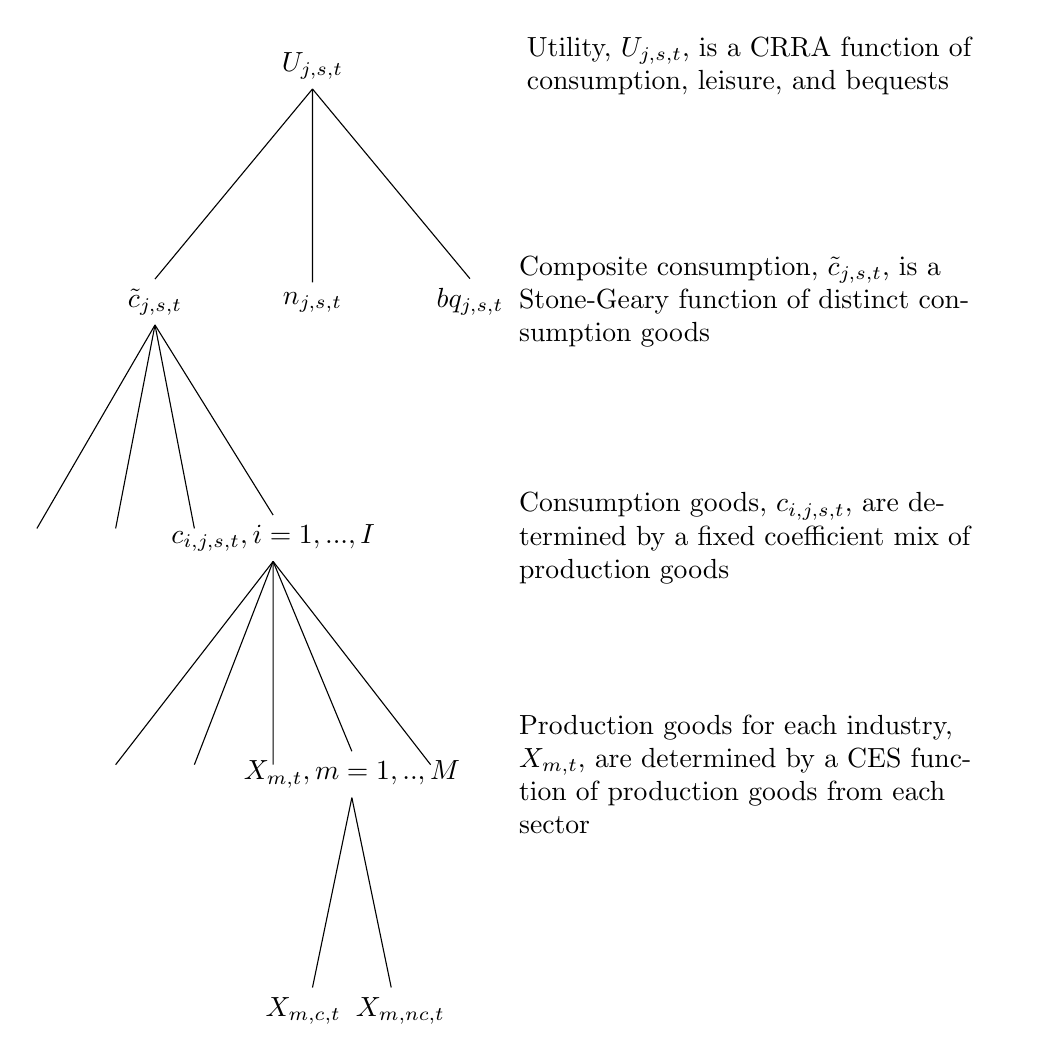
\begin{tikzpicture}
\tikzstyle{every node}=[auto,every node/.style={rectangle,draw, text centered, text width=1.3cm,minimum height=0.8cm },node distance=3cm]
\tikzset{%
level 1/.style={sibling distance = 2cm, level distance=3cm,edge from parent path={(\tikzparentnode.south) -- (\tikzchildnode.north)}},
level 2/.style={sibling distance = 1cm,level distance=3cm}
%level 4/.style={sibling distance = 1.1cm,level distance=3cm}
}
  \node (0){$U_{j,s,t}$}
    child {node (1) {$\tilde{c}_{j,s,t}$}
    child {node {}}
    child {node {}}
    child {node {}}
    child {node (2){$c_{i,j,s,t}, i=1,...,I$}   
child {node (3) {}}
            child {node {}}
            child {node {}}
            child {node {$X_{m,t}, m=1,..,M$}       
             child {node {$X_{m,c,t} \ \ $}}
             child {node {$\ \ X_{m,nc,t}$}}}
             child {node {}}
                        }
                  }
child {node {$n_{j,s,t}$}}
child {node {$bq_{j,s,t}$}} ;

\node at (0) [xshift=+2.6cm,right,draw=none, text width=6cm]{Utility, $U_{j,s,t}$, is a CRRA function of consumption, leisure, and bequests};
\node at (1) [xshift=+4.5cm, right,draw=none, text width=6cm]{Composite consumption, $\tilde{c}_{j,s,t}$, is a Stone-Geary function of distinct consumption goods};
\node at (2) [xshift=+3.0cm, right,draw=none, text width=6cm]{Consumption goods, $c_{i,j,s,t}$, are determined by a fixed coefficient mix of production goods };
\node at (3) [xshift=+5.0cm, right,draw=none, text width=6cm]{Production goods for each industry, $X_{m,t}$, are determined by a CES function of production goods from each sector};
\end{tikzpicture}
\end{figure}


    Households choose consumption of a composite consumption good, $c_{j,s+u,t+u}$, labor supply, $n_{j,s+u,t+u},$ and asset holdings, $b_{j,s+u+1,t+u+1}$, to maximize the expected, discounted, lifetime utility subject to their per-period budget constraint.  Total consumption of the composite good is made up of discretionary consumption, $\tilde{c}_{j,s,t}$, and minimum required purchases of each consumption good, $\bar{c}_{i,s}$.  Thus the consumer's choice is over $\tilde{c}_{j,s,t}$, which together with the minimum required purchases equal determine total composite consumption: $c_{j,s,t}=\tilde{c}_{j,s,t}+\sum_{i=1}^{I}c_{i,s}$.  It is therefore the case that there minimum required purchases affect the household's ability to smooth consumption over time.  We discuss the composite consumption good in more detail in Section \ref{sec:subutil}.  This composite good is age dependent, thus the price of the composite consumption good varies with age $s$.  We denote the gross-of-tax price of the composite consumption good for households of age $s$ in period $t$ as $\tilde{p}_{s,t}$ and the gross-of-tax price for good $i$ at time $t$ as $p_{i,t}$. The households' per period budget constraint is:
    
    \begin{equation}\label{EqBC}
      \begin{split}
        \sum_{i=1}^{I} p_{i,t}\bar{c}_{i,s} + \tilde{p}_{s,t}\tilde{c}_{s,t} + b_{j,s+1,t+1} \leq \left(1 + r_t\right) b_{j,s,t} + w_t e_{j,s}&n_{j,s,t} + \frac{BQ_{j,t}}{\lambda_j\tilde{N}_t} - T_{j,s,t} \\
        \quad\text{where}\quad b_{j,s,1} = 0 \\
        &\text{for} \quad E+1\leq s \leq E+S \quad \forall j,t
      \end{split}
    \end{equation}

\noindent\noindent Here, $r_{t}$ and $w_{t}$ are the real interest rate and the wages rate on a unit of effective labor.  The variable $e_{j,s}$ denotes the effective labor units of an individual from lifetime income group $s$ and age $j$.  An individual's labor income is thus determined by her choice of $n_{j,s,t}$ units of labor times her measure of effective labor units, $e_{j,s}$, times the wage per unit of effect labor.  An individuals effective labor units vary over the life-cycle, as the age subscript implies.  $BQ_{j,t}$ denote aggregate bequests left from those in lifetime income group {j} at time {t}.  We divide this number by the number of individuals in lifetime income group $j$ at time $t$, given by $\lambda_{j}\tilde{N}_{t}$, to determine the amount of bequests received by each household in lifetime income group $j$.\footnote{This distribution of bequests is just place holder. The goal is to find suitable data to calibrate the process describing the transmission of bequests between individuals of different ages and lifetime income groups.}  The last term in the budget constraint, $T_{j,s,t}$ are total taxes paid by the individual.  These include all non-consumption taxes and are based on tax functions for separate tax sources that we estimate based on a microsimulation model.  We discuss the parameterization and calibration of these functions below. 

    The Lagrangian for the individual's problem can be written as:
     \begin{equation}\label{eqn:hh_prob_lagrangian}
      \begin{split}
     \mathcal{L} =  \max_{\left\{ \substack{\tilde{c}_{j,s+u,t+u},\\\ {n}_{j,s+u,t+u},\\\ {b}_{j,s+u,t+u}}\right\}_{u=0}^{E+S-s}}  &  \sum_{u=0}^{E+S-s}\beta^u\left[\prod_{v=s-1}^{s+u-1}(1-\rho_v)\right]  \frac{\left(c_{j,s+u,t+u}\right)^{1-\sigma} - 1}{1-\sigma} + ...\\
  &   e^{g_y t(1-\sigma)}\chi^n_s+u\left(b\left[1 - \left(\frac{n_{j,s+u,t+u}}{\tilde{l}}\right)^\upsilon\right]^\frac{1}{\upsilon} + k\right) + \rho_s\chi^b\frac{\left(b_{j,s+u+1,t+u+1}\right)^{1-\sigma} - 1}{1-\sigma}  +... \\
       & \lambda_{j,s+u,t+u}\left\{ (1+r_{t+u})b_{j,s+u,t+u} + w_{t+u}e_{j,s+u}n_{j,s+u,t+u}+\frac{BQ_{j,t+u}}{\lambda_{j}\tilde{N}_{t+u}}-T_{j,s+u,t+u} -.... \right.\\
       & \left. \sum_{i=1}^{I}p_{i,t+u}\bar{c}_{i,s+u}-\tilde{p}_{s+u,t+u}\tilde{c}_{j,s+u,t+u} -b_{j,s+u+1,t+u+1} \right\}
        \end{split}
    \end{equation}
    
    
    
\noindent\noindent taking derivatives with respect to $\{\tilde{c}_{j,s,t},n_{j,s,t+u},b_{j,s,t+1}\}$ gives us the necessary conditions for each $j,s$ and $t$.  The necessary condition with respect to the discretionary consumption of the composite consumption good, $\tilde{c}_{j,s+u,t+u}$, labor supply, $n_{j,s+u,t+u}$, and asset holdings, $b_{j,s+u+1,t+u+1}$, are:
  
    \begin{equation}\label{Eqcfoc}
      \begin{split}
     \frac{\partial U}{\partial \tilde{c}_{j,s+u,t+u}}  = \beta^u\left[\prod_{v=s-1}^{s+u-1}(1-\rho_v)\right] c_{j,s+u,t+u}^{-\sigma} - \beta^u\left[\prod_{v=s-1}^{s+u-1}(1-\rho_v)\right]  \lambda_{j,s+u,t+u} \tilde{p}_{s+u,t+u} = 0, \forall u
        \end{split}
    \end{equation}

    \begin{equation}\label{Eqnfoc}
      \begin{split}
      \frac{\partial U}{\partial n_{j,s+u,t+u}} & = \beta^u\left[\prod_{v=s-1}^{s+u-1}(1-\rho_v)\right] e^{g_y (t+u)(1-\sigma)}\chi^n_{s}\biggl(\frac{b}{\tilde{l}}\biggr)\biggl(\frac{n_{j,s+u,t+u}}{\tilde{l}}\biggr)^{v-1}\Biggl[1 - \biggl(\frac{n_{j,s+u,t+u}}{\tilde{l}}\biggr)\Biggr]^{\frac{1-v}{v}} \\
      & -  \beta^u\left[\prod_{v=s-1}^{s+u-1}(1-\rho_v)\right]\lambda_{j,s+u,t+u} \left( w_{t+u} e_{j,s+u} - \frac{\partial T_{j,s+u,t+u}}{\partial n_{j,s+u,t+u}} \right)= 0, \forall u
        \end{split}
    \end{equation}

    \begin{equation}\label{Eqbfoc}
      \begin{split}
      \frac{\partial U}{\partial b_{j,s+u+1,t+u+1}} & = \beta^u\left[\prod_{v=s-1}^{s+u-1}(1-\rho_v)\right] \rho_s\chi^b\bigl(b_{j,s+u+1,t+u+1}\bigr)^{-\sigma} - \beta^u\left[\prod_{v=s-1}^{s+u-1}(1-\rho_v)\right] \lambda_{j,s+ut+u}  \\\ 
      & + \beta^{u+1}\left[\prod_{v=s-1}^{s+u}(1-\rho_v)\right] \lambda_{j,s+u+1,t+u+1} \left( 1 + r_{t+u+1} - \frac{\partial T_{j,s+u+1,t+u+1}}{\partial b_{j,s+u+1,t+u+1}} \right)= 0, \forall u
      \end{split}
    \end{equation}

 Note that the term $\frac{\partial T_{j,s+u+1,t+u+1}}{\partial n_{j,s+U+1,t+u+1}}$ give the change in total taxes for additional labor supply $\frac{\partial T_{j,s+u+1,t+u+1}}{\partial b_{j,s+U+1,t+u+1}}$ gives the change in total taxes for additional savings.  The tax functions that define the total taxes paid will take into account the interactions, for example how increasing capital income by saving more impacts the marginal tax rate on labor income in a system that progressively taxes labor income.  Rearranging the equations above to solve each for $\lambda_{t+u}$, we get the following:
    \begin{equation}
      \begin{split}
      \lambda_{j,s+u,t+u} = \frac{c_{j,s+u,t+u}^{-\sigma}}{\tilde{p}_{s,t+u}} \nonumber
      \end{split}
    \end{equation}

    \begin{equation}
      \begin{split}
      \lambda_{j,s+u,t+u} = \frac{e^{g_y (t+u)(1-\sigma)}\chi^n_{s}\biggl(\frac{b}{\tilde{l}}\biggr)\biggl(\frac{n_{j,s+u,t+u}}{\tilde{l}}\biggr)^{v-1}\Biggl[1 - \biggl(\frac{n_{j,s+u,t+u}}{\tilde{l}}\biggr)\Biggr]^{\frac{1-v}{v}}}{ w_{+u} e_{j,s+u} - \frac{\partial T_{j,s+u,t+u}}{\partial n_{j,s+u,t+u}} }  \nonumber
      \end{split}
    \end{equation}

    \begin{equation}
      \begin{split}
      \lambda_{j,s+u,t+u} = \rho_s\chi^b\bigl(b_{j,s+u+1,t+u+1}\bigr)^{-\sigma} - \beta (1-\rho_{s+u}) \lambda_{t+u+1} \left( 1 + r_{t+u+1} - \frac{\partial T_{j,s+u+1,t+u+1}}{\partial b_{j,s+u+1,t+u+1}} \right)
        \end{split}  \nonumber
    \end{equation}

    These three equations can then be reduced to just two equations that must hold for all $j,s,$ and $t$.  The first relates the marginal utility of consumption of the composite good to the marginal utility of labor:
    \begin{equation}\label{EqcEuler}
      \begin{split}
      & \frac{ c_{j,s+u,t+u}^{-\sigma}}{\tilde{p}_{s+u,t+u}} \\
      & = \frac{ e^{g_y (t+u)(1-\sigma)}\chi^n_{s}\biggl(\frac{b}{\tilde{l}}\biggr)\biggl(\frac{n_{j,s+u,t+u}}{\tilde{l}}\biggr)^{v-1}\Biggl[1 - \biggl(\frac{n_{j,s+u,t+u}}{\tilde{l}}\biggr)\Biggr]^{\frac{1-v}{v}} } { w_{t+u} e_{j,s+u} - \frac{\partial T_{j,s+u,t+u}}{\partial n_{j,s+u,t+u}} }
       \end{split}
    \end{equation}

    \noindent\noindent The second equation is the intertemporal Euler equation for savings, including the utility effects of bequests:
    \begin{equation}\label{EqbEuler}
      \begin{split}
      & \frac{ c_{j,s+u,t+u}^{-\sigma}}{\tilde{p}_{s+u,t+u}} = \rho_s\chi^b\bigl(b_{j,s+u+1,t+u+1}\bigr)^{-\sigma}  + \frac{ \beta(1-\rho_{s+u}) c_{j,s+u+1,t+u+1}^{-\sigma}} {\tilde{p}_{s+u+1,t+u+1}} \times \left( 1 + r_{t+u+1} - \frac{\partial T_{j,s+u+1,t+u+1}}{\partial b_{j,s+u+1,t+u+1}} \right)
      \end{split}
    \end{equation}

   
    \subsection{Household's Portfolio Problem}\label{sec:portfolio}
    
Household's are assumed to have constant elasticity of substitution (CES) preferences over debt and equity in their portfolio.  These preferences allows for investor portfolios that are a mix of debt and equity despsite the two assets having differential returns.  Thus, while our model does not include idiosyncratic or aggregate uncertainty, these CES preferences account for the premium paid to the more risky assets through the preference parameters. To match lifecycle portfolio changes, we may consider allowing to the CES preference parameters to vary by age.  Given the CES preferences, the household's total assets, $a_{j,s,t}$ are given by (\textcolor{red}{NOTE that if we include these notations we should change our notation for assets from $b$ to $a$. We need to also think about the notion for equity - I use $e$ below, but we are already using that for effective labor units.}): 

\begin{equation}
\label{eqn:ces_port}
a_{j,s,t}= \left[\gamma_{a,s}^{\frac{-1}{\ve_{a,s}}}b_{j,s,t}^{\frac{1+\ve_{a.s}}{\ve_{a,s}}}+(1-\gamma_{a,s})^{\frac{-1}{\ve_{a,s}}}e_{j,s,t}^{\frac{1+\ve_{a,s}}{\ve_{a,s}}}\right]^{\frac{\ve_{a,s}}{1+\ve_{a,s}}}
\end{equation}
    
The parameter $\ve_{a,s}$ is the elasticity of substitution between bonds and stocks in the asset portfolio of an age $s$ household.  $\gamma_{a,s}$ is the taste parameter in these preferences (\textcolor{red}{I've written this in the most flexible way, where both parameters depend upon age, but perhaps we just want the taste parameter to vary by age the rate of substitution is constant.}).

Since neither firms of governments default in our model, the rate of return on bonds issued by firms and government will all have the same pretax rate of return, $r_{b,t}$.  

It's not clear whether firm equity will all have the same return.  It seems that multinationals, with the ability to shift profits, may have higher returns than domestic corporations.  In general, firms will earn economic profits and thus have a rate of return in excess of the risk free return, $r_{b,t}$.  If it is the case that some firms earn greater returns than others, I think we may just assume that households own an diversified equity portfolio of all firms and thus earn the average return on equity.  Thus we'll have either a market return for equity that is the average of the heterogeneous returns across firms or the return that is the same for all firms.  We will denote the pretax market turn on equity as $r_{e,t}$.

We introduce further notation that is the after-tax gross return on the each asset composite.  The after-tax gross return on bonds for a household of age $s$, lifetime income group $j$, and in year $t$ is given by:

\begin{equation}
\rho_{b,j,s,t}=(1+r_{b,t}(1-\tau^{int}(y_{j,s,t})))
\end{equation}

\textcolor{red}{Note that I've again shifted some notation.  We had used $a$ to denote total income for tax purposes, while I use $y$ above (since I've used $a$ for total assets).  Also, I'm writing the marginal tax rate on interest income as a function of total income, $\tau^{int}(y_{j,s,t})$, rather than using the total tax function.  I think this is helpful for expository purposes.  Is it ok to use the marginal rather than the average tax function?  Seems like we could use either interchangeably.  But if we want to use the total tax function, the notation for the above would be: } 

\begin{equation}
\rho_{b,j,s,t}=(1+r_{b,t}) - \frac{\partial T_{j,s,t}}{\partial b_{j,s,t}}
\end{equation}

\textcolor{red}{Either way, we'll want to be sure that when we calibrate this functions we account for the mix of tax exempt and taxable interests realized by household and how that changes across age and income group.  The micro simulation model should be able to help us here.}


The after-tax gross return on equity for a household of age $s$, lifetime income group $j$, and in year $t$ is given by:

\begin{equation}
\rho_{e,j,s,t}=(1+r_{e,t}(1-\tau^{cap}(y_{j,s,t})))
\end{equation}

Here, $\tau^{cap}$ will be the tax rate on capital income - some mix of the tax on dividends and capital gains from corporate and non-corporate entities.  Recall that we do not explicitly model capital gains realizations nor do we track dividend issues from each representative firm.  Instead, the return to the firms (both from dividends and capital gains) is put into the per period return on equity, $r_{e,t}$.  Thus the tax rate on these returns must be a weighted average of the taxes on dividends and capital gains, where the weighting is given by data on the share of income from capital gains and dividends by age and income group in the data.

We can now write the gross after-tax return on the households total portfolio:

\begin{equation}
\label{eqn:port_return}
\rho_{a,j,s,t}a_{j,s,t}=\rho_{b,j,s,t}b_{j,s,t}+\rho_{e,j,s,t}e_{j,s,t}
\end{equation}

The optimal portfolio is given by the household choosing bonds and stocks to maximize Equation \ref{eqn:port_return} subject to Equation \ref{eqn:ces_port}.  The Lagrangian for this problem is:

\begin{equation}
\mathcal{L} =  \max_{b_{j,s,t},e_{j,s,t}} \rho_{b,j,s,t}b_{j,s,t} + \rho_{e,j,s,t}e_{j,s,t} + \lambda_{j,s,t}\left(a_{j,s,t} -  \left[\gamma_{a,s}^{\frac{-1}{\ve_{a,s}}}b_{j,s,t}^{\frac{1+\ve_{a.s}}{\ve_{a,s}}}+(1-\gamma_{a,s})^{\frac{-1}{\ve_{a,s}}}e_{j,s,t}^{\frac{1+\ve_{a,s}}{\ve_{a,s}}}\right]^{\frac{\ve_{a,s}}{1+\ve_{a,s}}}\right)
\end{equation}

Since every variable is subscripted by $j,s,t$ we drop these and write the necessary conditions as:

\begin{equation}
\label{eqn:port_foc_b}
\frac{\partial \mathcal{L}}{\partial b}: \rho_{b} = \lambda \gamma_{a,s}^{\frac{-1}{\ve_{a,s}}}b^{\frac{1}{\ve_{a,s}}}\left[\gamma_{a,s}^{\frac{-1}{\ve_{a,s}}}b^{\frac{1+\ve_{a.s}}{\ve_{a,s}}}+(1-\gamma_{a,s})^{\frac{-1}{\ve_{a,s}}}e^{\frac{1+\ve_{a,s}}{\ve_{a,s}}}\right]^{\frac{-1}{1+\ve_{a,s}}}
\end{equation}

\begin{equation}
\label{eqn:port_foc_e}
\frac{\partial \mathcal{L}}{\partial e}: \rho_{e} = \lambda (1- \gamma_{a,s})^{\frac{-1}{\ve_{a,s}}}e^{\frac{1}{\ve_{a,s}}}\left[\gamma_{a,s}^{\frac{-1}{\ve_{a,s}}}b^{\frac{1+\ve_{a.s}}{\ve_{a,s}}}+(1-\gamma_{a,s})^{\frac{-1}{\ve_{a,s}}}e^{\frac{1+\ve_{a,s}}{\ve_{a,s}}}\right]^{\frac{-1}{1+\ve_{a,s}}}
\end{equation}
       
\begin{equation}
\label{eqn:port_foc_lambda}
\frac{\partial \mathcal{L}}{\partial \lambda}: a = \left[\gamma_{a,s}^{\frac{-1}{\ve_{a,s}}}b^{\frac{1+\ve_{a.s}}{\ve_{a,s}}}+(1-\gamma_{a,s})^{\frac{-1}{\ve_{a,s}}}e^{\frac{1+\ve_{a,s}}{\ve_{a,s}}}\right]^{\frac{\ve_{a,s}}{1+\ve_{a,s}}}
\end{equation}
              
We can use Equations \ref{eqn:port_foc_b} and \ref{eqn:port_foc_e} to find the ratio of bonds to stocks as (again, suppressing the subscripts):

\begin{equation}
\label{eqn:port_ratio}
\frac{b}{e}= \left(\frac{\rho_{b}}{\rho_{e}}\right)^{\ve_{a,s}}\frac{\gamma_{a,s}}{(1-\gamma_{a,s})}
\end{equation}
     
Using Equation \ref{eqn:port_ratio} can then be used with \ref{eqn:port_foc_lambda} to find demand for bonds and stocks separately.  The solution should yield (\textcolor{red}{We should work this out here, I had some trouble, but we know what the solution should be...}):

\begin{equation}
\label{eqn:bond_demand}
b_{j,s,t} = \left(\frac{\rho_{b,j,s,t}}{\rho_{e,j,s,t}}\right)^{\ve_{a,s}}\gamma_{a,s}a_{j,s,t}
\end{equation}     

\begin{equation}
\label{eqn:equity_demand}
e_{j,s,t} = \left(\frac{\rho_{e,j,s,t}}{\rho_{b,j,s,t}}\right)^{\ve_{a,s}}(1-\gamma_{a,s})a_{j,s,t}
\end{equation}     

We can thus find the return to the portfolio as:

\begin{equation}
\label{eqn:port_return}
\rho_{a,j,s,t} = \left(\gamma_{a,s}\rho_{b,j,s,t}^{\ve_{a,s}}+(1-\gamma_{a,s})\rho_{e,j,s,t}^{\ve_{a,s}}\right)^{\frac{1}{1+\ve_{a,s}}}
\end{equation}     

\subsubsection{After-tax return differentials}

I don't think we have any problem in that household have different after tax returns.  Each will hold a different portfolio because of this, but none will have corner solutions because of the CES preferences.  So it's not problem if, for example, the after-tax return to stocks exceed the return to bonds.  This just means households hold relatively more stocks.  

When considering the firms' problems we do need to think about different household having different after-tax returns to equity.  The solution there will be that the firms just chooses a representative household when thinking about maximizing firm value.  The household will be termed the ``marginal investor".  However, we will need to think a bit about which household in the microsimulation model represents this investor.
       
       
    \subsection{Household's Subutility Function}\label{sec:subutil}
    
    Household preferences over the composite consumption good are modeled as a Stone-Geary function. The aggregate discretionary consumption of the composite good is defined as follows.
    \begin{equation} \label{eqn:comp_cons}
        \tilde{c}_{j,s,t}  = \prod_{i=1}^I \left( c_{i,j,s,t} - \bar c_{i,s} \right) ^{\alpha_{i,s}} 
    \end{equation}

Where, $c_{i,j,s,t}$ is consumption of good $i$ by household of type $j$, age $s$, at time $t$.  There are $I$ total goods and $\bar{c}_{i,s}$ represents the minimum consumption amount for each good at each age.  The parameters $\alpha_{i,s}$ are the share parameters (and $\sum_{i=1}^{I} \alpha_{i,s}=1$).  They correspond to the share of income, after minimum expenditure amounts, that are spent on each good at each age.  Allowing the minimum consumption amounts and the share parameters to vary by age helps to incorporate life-cycle profiles of consumption into the model.  For example, we do not explicitly model household formation decisions, but they will be some of the effects of changes in household composition over the life-cycle are obtained through the parameters of the Stone-Geary function.  For example, the minimum required expenditure on shelter may be higher in the middle of the life-cycle when household size is larger.  The minimum consumption amounts also mean that the composition of consumption will vary with income, even though all households have the same utility function.

The consumer chooses $c_{i,j,s,t}$ to maximize Equation \ref{Eqcagg} subject to the budget constraint:

    \begin{equation} \label{eqn:cons_budgetcons}
        \sum_{i=1}^{I} p_{i,t}(c_{i,j,s,t}-\bar{c}_{i,s})  = \tilde{p}_{s,t}\tilde{c}_{j,s,t}
    \end{equation}

\noindent where $p_{i,t}$ is the gross of tax price of good $i$ at time $t$ and $\tilde{p}_{s,t}$ is the gross of tax price of the the discretionary component of the composite consumption good consumed by those of age $s$ at time $t$.  Maximization of \ref{Eqcagg} subject to \ref{eqn:cons_budgetcons} yields:

    \begin{equation} \label{eqn:cons_lagrangian}
       \mathcal{L} =  \max_{\{c_{i,j,s,t}\}_{i=1}^{I}}  \prod_{i=1}^I \left( c_{i,j,s,t} - \bar c_{i,s} \right) ^{\alpha_{i,s}}  + \lambda \left(\tilde{p}_{s,t}\tilde{c}_{j,s,t} - \sum_{i=1}^{I} p_{i,t}(c_{i,j,s,t}-\bar{c}_{i,j,s,t})\right)
    \end{equation}
    
    Which as $I$ FOCs (for each $j$, $s$, $t$):
    
      \begin{equation} \label{eqn:cons_FOC}
      \begin{split}
       & \frac{\partial \mathcal{L}}{\partial c_{i,j,s,t}} = \frac{\alpha_{i,s} \prod_{i=1}^I \left( c_{i,j,s,t} - \bar c_{i,s} \right) ^{\alpha_{i,s}}}{(c_{i,j,s,t}-\bar{c}_{i,s})}-\lambda p_{i,t} = 0, \forall \ i  \\
       & \implies  \frac{\alpha_{i,s} \prod_{i=1}^I \left( c_{i,j,s,t} - \bar c_{i,s} \right) ^{\alpha_{i,s}}}{(c_{i,j,s,t}-\bar{c}_{i,s})} = \lambda p_{i,t}, \forall \ i \\
       & \implies  \frac{\alpha_{i,s} \prod_{i=1}^I \left( c_{i,j,s,t} - \bar c_{i,s} \right) ^{\alpha_{i,s}}}{ p_{i,t}(c_{i,j,s,t}-\bar{c}_{i,s})} = \lambda, \forall \ i \\
       & \implies \frac{\alpha_{i,s}}{p_{i,t}(c_{i,j,s,t}-\bar{c}_{i,s})}=\frac{\alpha_{j,s}}{p_{k,t}(c_{k,j,s,t}-\bar{c}_{k,s})}, \forall \ i,k \\
       & \implies c_{i,j,s,t}= \frac{\alpha_{i,s} p_{k,t}(c_{k,j,s,t}-\bar{c}_{k,s})}{\alpha_{k,s} p_{i,t}} + \bar{c}_{i,s} \forall i,k 
       \end{split}
    \end{equation}
    
    Now substitute the last line of \ref{eqn:cons_FOC} into the budget constraint (Equation \ref{eqn:cons_budgetcons}):
    
          \begin{equation} \label{eqn:cons_solve}
      \begin{split}
       & \tilde{p}_{s,t}\tilde{c}_{j,s,t} = \sum_{i=1}^{I}p_{i,t}(c_{i,j,s,t}-\bar{c}_{i,s}) \\
       & \implies  \tilde{p}_{s,t}\tilde{c}_{j,s,t} = \sum_{i=1}^{I}p_{i,t}\left[ \frac{\alpha_{i,s} p_{k,t}(c_{k,j,s,t}-\bar{c}_{k,s})}{\alpha_{k,s} p_{i,t}} + \bar{c}_{i,s}- \bar{c}_{i,s}\right] \\
       & \implies  \tilde{p}_{s,t}\tilde{c}_{j,s,t} = \sum_{i=1}^{I}\left[ \frac{\alpha_{i,s} p_{k,t}(c_{k,s}-\bar{c}_{k,s})}{\alpha_{k,s}}\right] \\
       & \implies  \tilde{p}_{s,t}\tilde{c}_{j,s,t} = \frac{ p_{k,t}(c_{k,j,s,t}-\bar{c}_{k,s})}{\alpha_{k,s}} \underbrace{\sum_{i=1}^{I}\alpha_{i,s}}_{=1} \\	
        & \implies  \tilde{p}_{s,t}\tilde{c}_{j,s,t} = \frac{ p_{k,t}(c_{k,j,s,t}-\bar{c}_{k,s})}{\alpha_{k,s}} \\
        & \implies  \frac{ p_{k,t}(c_{k,j,s,t}-\bar{c}_{k,s})}{\alpha_{k,s}}  = \tilde{p}_{s,t}\tilde{c}_{j,s,t}   \\	
        & \implies  c_{k,j,s,t}  = \frac{\alpha_{k,s} \tilde{p}_{s,t}\tilde{c}_{j,s,t}}{p_{k,t}} + \bar{c}_{k,s},  \forall \ k  \\	
       \end{split}
    \end{equation}
    
    Thus, total consumption of each good $i$, $c_{i,j,s,t}$, is given by the the amount of minimum consumption plus the share of total expenditures remaining after making the minimum expenditures on all goods (this is called the ``supernumerary" expenditure).  We derive the prices of the age $s$ composite consumption good in period $t$, $\tilde{p}_{s,t}$ by using the demand for good $i$ provided in Equation \ref{cons_solve} in the function defining aggregate discretionary consumption, Equation \ref{eqn:comp_cons}: 
    
              \begin{equation} \label{eqn:composite_price}
      \begin{split}
      & \tilde{c}_{j,s,t} = \prod_{i=1}^{I}(c_{i,j,s,t}-\bar{c}_{i,s})^{\alpha_{i,s}} \\
      &\implies \tilde{c}_{j,s,t} = \prod_{i=1}^{I}\left( \frac{\alpha_{i,s} \tilde{p}_{s,t}\tilde{c}_{j,s,t}}{p_{i,t}} + \bar{c}_{i,s}-\bar{c}_{i,s}\right)^{\alpha_{i,s}} \\
      &\implies \tilde{c}_{j,s,t} = \prod_{i=1}^{I} \left( \frac{\alpha_{i,s} \tilde{p}_{s,t}\tilde{c}_{j,s,t}}{p_{i,t}} \right)^{\alpha_{i,s}} \\
      &\implies \tilde{c}_{j,s,t} =  \tilde{p}_{s,t}\tilde{c}_{j,s,t} \prod_{i=1}^{I}\left( \frac{\alpha_{i,s}}{p_{i,t}} \right)^{\alpha_{i,s}} \\
      &\implies \frac{\tilde{p}_{s,t}\tilde{c}_{j,s,t}}{\tilde{c}_{j,s,t}} =  \prod_{i=1}^{I}\left( \frac{p_{i,t}}{\alpha_{i,s}} \right)^{\alpha_{i,s}} \\
       &\implies \tilde{p}_{s,t} =  \prod_{i=1}^{I}\left( \frac{p_{i,t}}{\alpha_{i,s}} \right)^{\alpha_{i,s}} \\
       \end{split}
    \end{equation}
    
    This composite good price is then used in the household's intertemporal optimization problem described in Equation \ref{eqn:hh_prob_lagrangian}.  With the parameters and endogenous variables, we then use \ref{eqn:cons_solve} to find the $c_{i,j,s,t}$.
    
    \subsection{Relating Consumption and Production Goods}\label{sec:prod_cons_map}
    
    Our model contains $I$ consumption goods and $M$ production goods.  We denote the quantity of production good $m$ in period $t$ as $X_{m,t}$.  We relate the output of the production sectors and the consumption goods using a fixed coefficient model. That is, we assume each consumption good is made up of a mix of the outputs of different production sectors.  This means that the composition of these consumption goods do not respond to prices. The weights that determine the mix for each consumption goods are given in the matrix $\Pi$.  Element $\pi_{i,m}$ of the matrix $\Pi$ corresponds to the percentage contribute of the output of sector $m$ in the production of good $i$.  The total supply of good $i$ in the economy at time $t$ is thus given by: 
    
             \begin{equation} \label{eqn:mix_cons}
             c_{i,t} = \sum_{m=1}^{M}\pi_{i,m}X_{m,t} 
    	\end{equation}
	
 \noindent\noindent And the price of a unit of consumption good $i$ at time $t$ is:
	
             \begin{equation} \label{eqn:mix_cons_price}
             p_{i,t} = \sum_{m=1}^{M}\pi_{i,m}p_{m,t}, 
    	\end{equation}
    
    \noindent\noindent Where $p_{m}$ is the price of output of production sector $m$ at time $t$.
    
    \subsection{Preferences for Corporate vs. Noncorporate Goods}\label{sec:pref_corp_noncorp}
    
    Production sectors may contain corporate and non-corporate producers, each facing different tax treatment.  If the output from corporate and non-corporate entities are perfect substitutes, then if the producers have the same production technology, consumers will end up consuming only the output from the sector with lowest after tax cost of producing.  \citet{GK1989} propose a model where different production sectors use different technologies, which can give rise to an equilibrium where both the corporate and non-corporate sector produce the same good.  We take a different track, following \citet{FR1993} we allow production technologies to vary across industry, but not across sectors within industry.  Both sectors produce output in equilibrium, because output across sectors are not perfect substitutes.  For example, food outside the home from a corporate, chain restaurant chain is not the same as food outside the home from a small, family-owned restaurant.  Specifically, we define consumer preferences such that demand for the composite production good (combing output from the corporate and non-corporate sector) for production sector $m$ at time $t$, $X_{m,t}$, is a constant elasticity of substitution (CES) function of the output from the corporate and non-corporate sectors, $X_{m,t,C}$ and $X_{m,t,NC}$, respectively:
    
                  \begin{equation} \label{eqn:comp_output}
             X_{m,t} = \left[\gamma_{m}^{\frac{1}{\ve_{3}}}X_{m,t,C}^{\frac{(\ve_{3}-1)}{\ve_{3}}}+(1-\gamma_{m})^{\frac{1}{\ve_{3}}}X_{m,t,NC}^{\frac{(\ve_{3}-1)}{\ve_{3}}}+\right]^{\frac{\ve_{3}}{(\ve_{3}-1)}}, 
    	\end{equation}
	
	\noindent where $\ve_{3}$ is the elasticity of substitution between corporate and non-corporate output and is assumed to be constant across industries.  The share parameter in the CES function, $\gamma_{m}$ is allowed to vary across industry and will be identified by the fraction of corporate produced output across industries.  The CES function thus explains the existence of corporate and non-corporate production within each industry as well as the different shares of corporate output across industries.  Because of these preferences, changes in corporate and non-corproate tax treatment will have differential impacts across consumers of different ages and income levels.  
	Consumers choose $X_{m,t,C}$ and $X_{m,t,NC}$ to maximize \ref{eqn:comp_output} subject to:
	
	 \begin{equation} \label{eqn:comp_output_cons}
             p_{m,t}X_{m,t} = p_{m,t,C}X_{m,t,C}+p_{m,t,NC}X_{m,t,NC}, 
    	\end{equation}
	
	
\noindent where $p_{m,t,C}$ and $p_{m,t,NC}$ are the prices of output from the corporate and non-corporate firms in production industry $m$, respectively.  Note that these prices are determined through the firm's profit maximization problem and the zero economic profit condition for firms. The constrained optimization problem consumers face is: 
    
 \begin{equation} \label{eqn:comp_output_lagrangian}
	\begin{split}
	 \mathcal{L} = \left[\gamma_{m}^{\frac{1}{\ve_{3}}}X_{m,t,C}^{\frac{(\ve_{3}-1)}{\ve_{3}}}+(1-\gamma_{m})^{\frac{1}{\ve_{3}}}X_{m,t,NC}^{\frac{(\ve_{3}-1)}{\ve_{3}}}+\right]^{\frac{\ve_{3}}{(\ve_{3}-1)}} + \lambda_{m,t,C}\left(p_{m,t}X_{m,t} - p_{m,t,C}X_{m,t,C}+p_{m,t,NC}X_{m,t,NC}\right)
  	\end{split}
\end{equation}
    
    FOCs are:
    
\begin{equation} \label{eqn:comp_output_foc_C}
	\begin{split}
       	&  \frac{\partial \mathcal{L}}{\partial X_{m,t,C}} = \gamma_{m}^{\frac{1}{\ve_{3}}} X_{m,t,C}^{\frac{-1}{\ve_{3}}} \left[\gamma_{m}^{\frac{1}{\ve_{3}}}X_{m,t,C}^{\frac{(\ve_{3}-1)}{\ve_{3}}}+(1-\gamma_{m})^{\frac{1}{\ve_{3}}}X_{m,t,NC}^{\frac{(\ve_{3}-1)}{\ve_{3}}}+\right]^{\frac{1}{(\ve_{3}-1)}} - \lambda_{m,t,C} p_{m,t,C} = 0
      	 \end{split}
\end{equation}
    
   and
   
\begin{equation} \label{eqn:comp_output_foc_NC}
	\begin{split}
       	&  \frac{\partial \mathcal{L}}{\partial X_{m,t,NC}} = (1-\gamma_{m})^{\frac{1}{\ve_{3}}} X_{m,t,NC}^{\frac{-1}{\ve_{3}}} \left[\gamma_{m}^{\frac{1}{\ve_{3}}}X_{m,t,C}^{\frac{(\ve_{3}-1)}{\ve_{3}}}+(1-\gamma_{m})^{\frac{1}{\ve_{3}}}X_{m,t,NC}^{\frac{(\ve_{3}-1)}{\ve_{3}}}+\right]^{\frac{1}{(\ve_{3}-1)}} - \lambda_{m,t,C} p_{m,t,NC} = 0
	\end{split}
\end{equation}
    
    Solving the two necessary conditions, we can find the equations for the demand for the corporate and non-corporate output in industry $m$ as a function of the prices out output from each sector of industry $m$, price of the composite production good, the demand for the composite production good, and the parameters:
    
\begin{equation} \label{eqn:demand_XmtC}
	X_{m,t,C} = \frac{\gamma_{m}p_{m,t}X_{m,t}}{p_{m,t,C}^{\ve_{3}}\left[\gamma_{m}p_{m,t,C}^{1-\ve_{3}}+(1-\gamma_{m})p_{m,t,NC}^{1-\ve_{3}}\right]}
\end{equation}
    
    and 
    
    \begin{equation} \label{eqn:demand_XmtNC}
	X_{m,t,NC} = \frac{(1-\gamma_{m})p_{m,t}X_{m,t}}{p_{m,t,NC}^{\ve_{3}}\left[\gamma_{m}p_{m,t,C}^{1-\ve_{3}}+(1-\gamma_{m})p_{m,t,NC}^{1-\ve_{3}}\right]}
\end{equation}

To determine $p_{m,t}$, note that the CES subutility function defining preferences over corporate and non-corporate output within a production industry is linearly homogenous.  Because the subutility function is linearly homogenous, we know that the associated indirect utility function is homogenous of degree one in $X_{m,t}$.  Letting $V(\cdot)$ represent the indirect utility function, this means that $V(p_{m,t,C},p_{m,t,NC},\lambda X_{m,t}) = \lambda V(p_{m,t,C},p_{m,t,NC}, X_{m,t})$.  The linear homogeneity of the utility function also means that the indirect utility function is homogenous of degree -1 in prices.  That is, $V(\lambda p_{m,t,C},\lambda p_{m,t,NC}, X_{m,t}) = \frac{V(p_{m,t,C},p_{m,t,NC}, X_{m,t})}{\lambda}$. Linear homogeneity of the utility function means that: 

\begin{equation}
V(p_{m,t,C},p_{m,t,NC}, X_{m,t}) = \frac{p_{m,t}X_{m,t}}{e(p_{m,t,C},p_{m,t,NC})},
\end{equation}
    
    
\noindent\noindent where $e(p_{m,t,C},p_{m,t,NC})$ is the minimum expenditure for a unit of the composite good given prices.  Rearranging, we have: 
    
 \begin{equation}
 \label{eqn:price_comp}
 \begin{split}
& e(p_{m,t,C},p_{m,t,NC}) = \frac{p_{m,t}X_{m,t}}{V(p_{m,t,C},p_{m,t,NC}, X_{m,t})}\\
&\implies e(p_{m,t,C},p_{m,t,NC}) = p_{m,t}X_{m,t}/ \\
& {\left[\gamma_{m}^{\frac{1}{\ve_{3}}}\left( \frac{\gamma_{m}p_{m,t}X_{m,t}}{p_{m,t,C}^{\ve_{3}}\left[\gamma_{m}p_{m,t,C}^{1-\ve_{3}}+(1-\gamma_{m})p_{m,t,NC}^{1-\ve_{3}}\right]}\right)^{\frac{(\ve_{3}-1)}{\ve_{3}}}+(1-\gamma_{m})^{\frac{1}{\ve_{3}}}\left(\frac{(1-\gamma_{m})p_{m,t}X_{m,t}}{p_{m,t,NC}^{\ve_{3}}\left[\gamma_{m}p_{m,t,C}^{1-\ve_{3}}+(1-\gamma_{m})p_{m,t,NC}^{1-\ve_{3}}\right]}\right)^{\frac{(\ve_{3}-1)}{\ve_{3}}}+\right]^{\frac{\ve_{3}}{(\ve_{3}-1)}}}\\
&\implies e(p_{m,t,C},p_{m,t,NC}) = p_{m,t}X_{m,t}/ \\
& {p_{m,t}X_{m,t}\left[\gamma_{m}^{\frac{1}{\ve_{3}}}\left( \frac{\gamma_{m}}{p_{m,t,C}^{\ve_{3}}\left[\gamma_{m}p_{m,t,C}^{1-\ve_{3}}+(1-\gamma_{m})p_{m,t,NC}^{1-\ve_{3}}\right]}\right)^{\frac{(\ve_{3}-1)}{\ve_{3}}}+(1-\gamma_{m})^{\frac{1}{\ve_{3}}}\left(\frac{(1-\gamma_{m})}{p_{m,t,NC}^{\ve_{3}}\left[\gamma_{m}p_{m,t,C}^{1-\ve_{3}}+(1-\gamma_{m})p_{m,t,NC}^{1-\ve_{3}}\right]}\right)^{\frac{(\ve_{3}-1)}{\ve_{3}}}+\right]^{\frac{\ve_{3}}{(\ve_{3}-1)}}}\\
&\implies e(p_{m,t,C},p_{m,t,NC}) = 1/ \\
& \left[\gamma_{m}p_{m,t,C}^{1-\ve_{3}}+(1-\gamma_{m})p_{m,t,NC}^{1-\ve_{3}}\right]{\left[\gamma_{m}^{\frac{1}{\ve_{3}}}\left( \frac{\gamma_{m}}{p_{m,t,C}^{\ve_{3}}}\right)^{\frac{(\ve_{3}-1)}{\ve_{3}}}+(1-\gamma_{m})^{\frac{1}{\ve_{3}}}\left(\frac{(1-\gamma_{m})}{p_{m,t,NC}^{\ve_{3}}}\right)^{\frac{(\ve_{3}-1)}{\ve_{3}}}+\right]^{\frac{\ve_{3}}{(\ve_{3}-1)}}}\\
&\implies e(p_{m,t,C},p_{m,t,NC}) = 
\frac{\left[\gamma_{m}^{\frac{1}{\ve_{3}}}\left( \frac{\gamma_{m}}{p_{m,t,C}^{\ve_{3}}}\right)^{\frac{(\ve_{3}-1)}{\ve_{3}}}+(1-\gamma_{m})^{\frac{1}{\ve_{3}}}\left(\frac{(1-\gamma_{m})}{p_{m,t,NC}^{\ve_{3}}}\right)^{\frac{(\ve_{3}-1)}{\ve_{3}}}+\right]^{\frac{\ve_{3}}{(1-\ve_{3})}}}{\left[\gamma_{m}p_{m,t,C}^{1-\ve_{3}}+(1-\gamma_{m})p_{m,t,NC}^{1-\ve_{3}}\right]}\\
&\implies e(p_{m,t,C},p_{m,t,NC}) = 
\frac{\left[\gamma_{m}\left( \frac{1}{p_{m,t,C}^{\ve_{3}}}\right)^{\frac{(\ve_{3}-1)}{\ve_{3}}}+(1-\gamma_{m})\left(\frac{1}{p_{m,t,NC}^{\ve_{3}}}\right)^{\frac{(\ve_{3}-1)}{\ve_{3}}}+\right]^{\frac{\ve_{3}}{(1-\ve_{3})}}}{\left[\gamma_{m}p_{m,t,C}^{1-\ve_{3}}+(1-\gamma_{m})p_{m,t,NC}^{1-\ve_{3}}\right]}\\
&\implies e(p_{m,t,C},p_{m,t,NC}) = 
\frac{\left[\gamma_{m}p_{m,t,C}^{1-\ve_{3}}+(1-\gamma_{m})p_{m,t,NC}^{1-\ve_{3}}\right]^{\frac{\ve_{3}}{(1-\ve_{3})}}}{\left[\gamma_{m}p_{m,t,C}^{1-\ve_{3}}+(1-\gamma_{m})p_{m,t,NC}^{1-\ve_{3}}\right]}\\
&\implies e(p_{m,t,C},p_{m,t,NC}) = 
\left[\gamma_{m}p_{m,t,C}^{1-\ve_{3}}+(1-\gamma_{m})p_{m,t,NC}^{1-\ve_{3}}\right]^{\frac{1}{(1-\ve_{3})}}\\
\end{split}
\end{equation}   

\noindent\noindent Thus we have the price of the corporate-non-corporate composite good from production industry $m$ at time $t$ as:
\begin{equation}
 e(p_{m,t,C},p_{m,t,NC})=p_{m,t}=\left[\gamma_{m}p_{m,t,C}^{1-\ve_{3}}+(1-\gamma_{m})p_{m,t,NC}^{1-\ve_{3}}\right]^{\frac{1}{(1-\ve_{3})}}
 \end{equation}
 
%\textcolor{red}{I'm not sure, but I think we then have  $e(p_{m,t,C},p_{m,t,NC})=p_{m,t}$ since the unit of ``utility" is really a unit of output of the composite production good, $X_{m,t}$}.


    
    

\chapter{Firms}
\label{chap:firms}
\index{Firms%
@\emph{Firms}}%



\section{Firms}

There at least one representative firm for each production industry.  Most industries will have a both corporate and non-corporate firms.  Corporate firms may be as many as three - with a domestic corporation, a multi-national parent corporation, and a multi-national subsidiary corporation (the follows the structure of the CORTAX model in terms of the types of corporations).  However, for computational and calibration issues, we will simplify and have just a single multinational corporation for each production industry.  The extent of overseas operations will be a an element of calibration - therefore the degree to which each industries firm is multinational will vary across industry.  

The costs of making this simplification is that it would be more difficult to handle legislation about corporate inversion (but even that isn't handled well in the CORTAX structure).  It also makes it more difficult to do multi-country interactions of tax policy, which is what CORTAX is designed for.  I think out other features, such as a diverse set of industries and corporate and non-corporate firms, are more relevant for US tax policy and are difficult to fit in the CORTAX framework due to computational and calibration issues.

We start by describing a fully domestic corporate firm and it's optimal investment, employment, and financial policies.  We then add the international components that describe the multinational nature of this firm.  Next, we discuss the problem of the non-corporate firm.   The functional forms describing the technologies and constraints of the firms are the same across industry, but the parameter values (of both the policy variant and policy invariant) parameters may vary across sector.  In the notation below, we drop the industry subscripts for clarify of exposition.

\section{The Problem of the Domestic Corporation}

The objective of the firm is to maximize firm value.  Firms do this by choosing investment and labor demand, as well as financial policies such as new equity issues, dividend distributions, and borrowing.  There are a total of six endogenous variables in the domestic corporation's problem: investment demand ($I$), demand of effective labor units ($EL$), the stock of corporate debt ($B$), the amount of new equity issues ($VN$), dividend distributions, $DIV$, and the price of output ($p$).  The firm makes choices over the first five of these variables.  The last is determined by an assumption about market structure.  In particular, we assume that firms have a decreasing returns to scale production function and thus realize economic profits.  \textcolor{red}{We pin down the price of output by assuming that there is free entry into the market.  Thus, firms must set price at marginal cost.  With a decreasing returns to scale function, such a price still produces economic profits.  This condition then provides the final equation to identify our six exogenous variables.} 



\textcolor{red}{One issue to be resolved is how we handle differential returns on equity across industry and corporate/non-corporate status.  For example, the returns to some firms might differ because they have more overseas profits and/or more ability to shift income overseas to avoid US taxation.}

\subsection{The Value of the Firm}

The household's portfolio problem described in Section \ref{sec:portfolio} allows for differential returns on debt and equity.  It also makes clear that after tax returns differ across savers as they face different tax treatment.  In the formulation of the value of the firm, we use the tax rate on the marginal investor.  \textcolor{red}{It is an open question as to who this investor is, but we will take it to be the domestic investor with the median amount of savings.}  Noting that all individual level tax rates represent those on this marginal investor, we can derive the value of the firm in period $t$, $V_{t}$ in the following way.  The after-tax return on firm equity in period $t$ is given by:

\begin{equation}
\label{eqn:equity_return}
r_{e,t} = \frac{(1-\tau^{d}_{t})DIV_{t}+(1-\tau^{g}_{t})(V_{t+1}-V_{t}-VN_{t})}{V_{t}},
\end{equation} 

\noindent\noindent where  $VN_{t}$ are new equity issues in period $t$ (that dilute the value of period $t$ shareholders) and $DIV_{t}$ are dividends distributed in period $t$. The policy parameters $\tau^{d}_{t}$ and $\tau^{g}$ are the period $t$ marginal tax rates on dividends and capital gains for the marginal investor.

\subsubsection{An aside on after-tax rates of return}

\textcolor{red}{Note that the notation for the return on equity differs from that in Section \ref{sec:portfolio}, where $r_{e,t}$ is the before tax return.  In the current section, $r_{e,t}$ denotes the after-tax return for the marginal investor.  To the after-tax return for all investors, we have two options.  First, we can use the decision rules of firms (which imply dividend distributions an firm value) to find the pre-tax rate of return, call it $r^{pre}_{e,t}$:}

\begin{equation}
r^{pre}_{e,t}=\frac{DIV_{t}+V_{t+1}-V_{t}-VN_{t}}{V_{t}},
\end{equation}

\noindent\noindent \textcolor{red}{We then define the gross, after-tax return for a individual of lifetime income group $j$, age $s$, in period $t$ as in Section \ref{sec:portfolio}: $\rho_{e,s,j,t}=(1+r^{pre}_{e,t}(1-\tau^{cap}(y_{j,s,t})))$.}

\textcolor{red}{A second way to do this would be to use the firms decision rules to find the after tax return for each investor:}

\begin{equation}
r_{e,j,s,t} = \frac{(1-\tau^{d}_{j,s,t})DIV_{t}+(1-\tau^{g}_{j,s,t})(V_{t+1}-V_{t}-VN_{t})}{V_{t}},
\end{equation} 

\noindent\noindent \textcolor{red}{where the gross, after-tax return would be described by $\rho_{e,s,j,t}=1+r_{e,j,s,t}$.}

\textcolor{red}{The main difference between the two methods is that the first allows for the model to include some elements of the dividend clientele hypothesis (depending on the detail on asset holdings imputed to the micro simulation model).  In particular, the tax rate, $\tau^{cap}(y_{j,s,t})$ would be calibrated from the microsimulation model and therefore would be a weighted average of the tax rates on dividends and capital gains for filers in a particular age-income group, where the weighting depends on the amount of capital gains versus dividend income for those filers.  In contract, the second method assumed that all households get the same mix of dividends and capital gain income.  However, the second method benefits from using the model's endogenous split between dividend and capital gains income, rather than assuming that the split is the same over time (but varies in the cross-section).  So, to summarize, the first method allows for cross-sectional variation in the split between dividend and capital gains income (but no variation over time within a filer type), while the second method allows for variation over time (but not across filer types).}

\subsection{The Value of the Firm, cont'd}
We can rearrange Equation \ref{eqn:equity_return} to solve for $V_{t}$:

\begin{equation}
\begin{split}
(1-\tau^{g}_{t})V_{t+1} &=V_{t}r_{e,t}-(1-\tau^{d}_{t})DIV_{t}+(1-\tau^{g}_{t})V_{t}+(1-\tau^{g}_{t})VN_{t}\\
\implies  V_{t+1} & = \frac{r_{e,t}V{t}-(1-\tau^{d}_{t})DIV_{t}}{(1-\tau^{g}_{t})}+V_{t}+VN_{t} \\
\implies  V_{t+1} & = V_{t}\left(\frac{r_{e,t}}{(1-\tau^{g}_{t})}+1\right)+VN_{t} - \left(\frac{1-\tau^{d}_{t}}{1-\tau^{g}_{t}}\right)DIV_{t} \\
\implies V_{t} &= \left(\frac{1}{1+\frac{r_{e,t}}{(1-\tau^{g}_{t})}}\right)\left[V_{t+1} - VN_{t} + \left(\frac{1-\tau^{d}_{t}}{1-\tau^{g}_{t}}\right)DIV_{t}\right]  \\
\end{split}
\end{equation}

\noindent\noindent Letting $ \left(\frac{1}{1+\frac{r_{e,t}}{(1-\tau^{g}_{t})}}\right) = 1+\theta_{t}$, we can solve for $V_{t}$ by repeatedly substituting for $V_{t+1}$ and applying the transversality condition ($\lim_{T \to \infty} \prod_{t=1}^{T}(1+\theta_{t})V_{T}=0$):

\begin{equation}
\label{eqn:solve_vs}
\begin{split}
& V_{t}=\frac{V_{t+1}}{(1+\theta_{t})} - \frac{VN_{t}}{(1+\theta_{t})}  + \frac{\left(\frac{1-\tau^{d}_{t}}{1-\tau^{g}_{t}}\right)DIV_{t}}{(1+\theta_{t})} \\
\implies &  V_{t}=\frac{V_{t+2}}{(1+\theta_{t})(1+\theta_{t+1})} - \frac{VN_{t+1}}{(1+\theta_{t})(1+\theta_{t+1})}  + \frac{\left(\frac{1-\tau^{d}_{t+1}}{1-\tau^{g}_{t+1}}\right)DIV_{t+1}}{(1+\theta_{t})(1+\theta_{t+1})} - \frac{VN_{t}}{(1+\theta_{t})}  + \frac{\left(\frac{1-\tau^{d}_{t}}{1-\tau^{g}_{t}}\right)DIV_{t}}{(1+\theta_{t})} \\
\implies &  V_{t}= \frac{V_{t+3}}{(1+\theta_{t})(1+\theta_{t+1})(1+\theta_{t+2})} - \frac{VN_{t+2}}{(1+\theta_{t})(1+\theta_{t+1})(1+\theta_{t+2})}  + \frac{\left(\frac{1-\tau^{d}_{t+2}}{1-\tau^{g}_{t+2}}\right)DIV_{t+2}}{(1+\theta_{t})(1+\theta_{t+1})(1+\theta_{t+2})} \\
& - \frac{VN_{t+1}}{(1+\theta_{t})(1+\theta_{t+1})}  + \frac{\left(\frac{1-\tau^{d}_{t+1}}{1-\tau^{g}_{t+1}}\right)DIV_{t+1}}{(1+\theta_{t})(1+\theta_{t+1})} - \frac{VN_{t}}{(1+\theta_{t})}  + \frac{\left(\frac{1-\tau^{d}_{t}}{1-\tau^{g}_{t}}\right)DIV_{t}}{(1+\theta_{t})} \\
& \text{and so on...} \\
\implies & V_{t}=\underbrace{\prod_{\nu=t}^{\infty}\left(\frac{1}{1+\theta_{\nu}}\right)V_{\infty}}_{=0 \text{ by transversality condition}} - \sum_{u=t}^{\infty} \prod_{\nu=t}^{u}\left(\frac{1}{1+\theta_{\nu}}\right)\left[VN_{u} - \left(\frac{1-\tau^{d}_{u}}{1-\tau^{g}_{u}}\right)DIV_{u}\right]\\
\implies & V_{t}= \sum_{u=t}^{\infty} \prod_{\nu=t}^{u}\left(\frac{1}{1+\theta_{\nu}}\right)\left[ \left(\frac{1-\tau^{d}_{u}}{1-\tau^{g}_{u}}\right)DIV_{u}-VN_{u}\right]\\
\end{split}
\end{equation}

\subsection{Firm Production}

Firm's combine capital, $K$, and effective labor, $EL$, with a fixed factor of production, $A$ to produce output, $X$.  We can think of the fixed factor of production as ``location specific capital".  It is fixed in the sense that its supply is perfectly inelastic.  It is location specific in the sense that it is proportional to the size of the population in the firm's home country at time $t$. \textcolor{red}{CORTAX documentation at first suggests this factor is chosen optimally by the firm, but there is not first order condition for this choice shown.  The documentation does state that this factor is paid its marginal product.  So there are only economic profits before you account for the return to this factor of production.  I'm also not sure if we need this fixed factor of production to be proportional to the population.  CORTAX says yes so that you don't have productivity differential arising from differences in country size.  They consider multi-country model, but only steady state.  Do we need something similar so productivity doesn't depend upon population at time $t$?}  We write the amount of output produced as a function of this fixed factor and the value added, $VA$, from the input of capital and labor:

\begin{equation}
X_{t} = A_{t}(VA_{t})^{\alpha_{v}},
\end{equation} 

\noindent\noindent where $\alpha_{v}$ is the share of output attributable to the firm's value added and the fixed factor of production is given by:

\begin{equation}
A_{t} = (A_{0,t}\omega_{t}N_{t})^{1-\alpha_{v}}
\end{equation}

\noindent\noindent  So the input from fixed factor of production used by the firm is given by the level of total factor productivity (TFP), $A_{0,t}$, and a exogenous share of the population, $N_{t}$ where the share is given by the parameter $\omega_{t}$ (\textcolor{red}{Not sure if we want this to vary by time, or just across production industry.}).  The share parameters must sum to one.  That is, $\sum_{m=1}^{M} \omega_{m,t} = 1$.     We assume that TFP grows at the same rate across industry, with the growth rate given by $g_{a}$.  The value added is given by a CES function:

\begin{equation}
\label{eqn:prod_fun}
F(A_{0,t},K_{t},EL_{t})=VA_{t} =A_{0,t} \left[(\gamma_{})^{1/\epsilon_{}}(K_{t})^{(\epsilon-1)/\epsilon_{}}+(1-\gamma_{})^{1/\epsilon_{}}(e^{g_{y}t}EL_{t})^{(\epsilon_{}-1)/\epsilon_{}}\right]^{(\epsilon_{}/(\epsilon_{}-1))},
\end{equation}

\noindent\noindent where $\epsilon$ gives the elasticity of substitution between capital and labor and $\gamma$ is the share parameter in the CES production function.  Effective labor units are affected by labor augmenting technological change.  The growth rate of this technology is give by $g_{y}$.  If $\alpha_{v}<1$, then the production function exhibits decreasing returns to scale with respect the firm's inputs of capital and labor.

We can derive the marginal products of capital and labor as:

\begin{equation}
\label{eqn:mpk}
MPK_{t}=\frac{\partial X_{t}}{\partial K_{t}}=A_{0,t}^{\frac{\epsilon-1}{\epsilon}} \left(\frac{\alpha_{v}X_{t}}{VA_{t}}\right)\left(\frac{\gamma VA_{t}}{K_{t}}\right)^{\frac{1}{\epsilon}}
\end{equation}

\begin{equation}
\label{eqn:mpl}
MPL_{t}=\frac{\partial X_{t}}{\partial EL_{t}}=A_{0,t}^{\frac{\epsilon-1}{\epsilon}} \left(\frac{\alpha_{v}X_{t}}{VA_{t}}\right)\left(\frac{(1-\gamma) VA_{t}}{EL_{t}}\right)^{\frac{1}{\epsilon}}
\end{equation}


\subsection{Firm Accounting}

Here we define a few accounting concepts and constraints relevant to the firm's problem.

\subsubsection{Cash Flow Constraint}
The firm's choices of investment and labor demand, as well as financial policies to finance these expenditures must satisfy the firm's cash flow constraint, which is given by:

\begin{equation}
\label{eqn:cash_flow}
\begin{split}
& \underbrace{p_{t}X_{t}+B_{t+1}+VN_{t}}_{\text{financial inflows}} =\\
 & \underbrace{w_{t}EL_{t} + (1+r_{b,t})B_{t} + c(B_{t+1},K_{t}) + p^{k}_{t}I_{t}(1+\Phi_{t}) + DIV_{t} + \tau^{p}_{t}p^{k}_{t}K_{t} + TE_{t} + \Psi(VN_{t})}_{\text{financial outflows}}
\end{split}
\end{equation}

\noindent\noindent Here, $p_{t}$ is the price of output, $B_{t+1}$ is the stock of debt at the beginning of period $t+1$ (so that new debt issues in period $t$ are equal to $B_{t+1}-B_{t}$), $VN_{t}$ are new equity issues (as noted above).  Labor costs are given by the wage rate times the number of effective labor units employed, $w_{t}EL_{t}$.  The interest rate of bond holdings is given by $r_{b,t}$ and the costs of holding debt are given by $c(B_{t+1},K_{t+1})$.  These costs might represent bankruptcy costs and other frictions in the debt markets.  The variable $p^{k}_{t}$ denotes the price of capital, $I_{t}$ represents investment, and $\Phi_{t}$ are the costs to adjusting the capital stock through new investment.  The firm also pays dividends, $DIV_{t}$, property taxes at a marginal rate of $\tau^{p}$ on the nominal value of its capital stock, income taxes $TE_{t}$, and costs to new equity issues, $\Psi(VN_{t})$.  Costs to new equity issues represent frictions in the equity markets such as those arising from information asymmetries. 

We impose to constraints on variables in the cash flow constraint: $DIV_{t}\geq0$ and $VN_{t}\geq0$.  In practice, firm's can and do buy back shares, but we restrict share repurchases in the model since the IRS treats share repurchases as dividends if they are done on a regular basis.  Our model therefore restricts the distribution of firm value to shareholders to be through dividend issues.  Note that we do not impose a constraint debt.  Positive values of $B$ indicate firm borrowing, while negative values represent firm saving.  Thus, retained earnings are held in the form of bonds that earn a rate of return $r_{b,t}$.

The law of motion of the capital stock is given by:
\begin{equation}
\label{eqn:lom_capital}
K_{t+1}=(1-\delta)K_{t} + I_{t},
\end{equation}

It is assumed that costs of debt take the following form:

\begin{equation}
\label{eqn:debt_cost}
c(B_{t+1},K_{t}) = \chi_{bk}\left(\frac{B_{t+1}}{K_{t}}\right)^{\ve_{bk}},
\end{equation}

\noindent\noindent where $\chi_{bk}$ is a scaling parameter and $\ve_{bk}$ is the curvature parameter. \textcolor{red}{Note the timing convention used here.  Leverage is determined by the current capital stock, not the one-period ahead capital stock.  While the investment made with the loan may be used as collateral for the loan, we assume that the costs of debt depend upon the ratio the loan to the current capital stock. This seems realistic if there is uncertainty about the potential value of the investments.  We will need to adjust this cost function in a way so that savings (i.e., $B<0$) result in no cost.}

Adjustment costs are assumed to be a quadratic function of deviations from the steady-state investment rate:
\begin{equation}
\label{eqn:adj_cost}
\Phi_{t}=\frac{\left(\frac{\beta}{2}\right)\left(\frac{I_{t}}{K_{t}}-\mu\right)^{2}}{\left(\frac{I_{t}}{K_{t}}\right)}
\end{equation}

\noindent\noindent The parameter $\beta$ is the scaling parameter for the adjustment cost function and $\mu$ is the steady-state investment rate, which is determined as $\mu=\delta+g_{y}+g_{n}$

Costs to new equity issues are assumed to be of the form:

\begin{equation}
\label{eqn:equity_cost}
\Psi(VN_{t})= \psi_{1}VN_{t} + \psi_{2}VN_{t}^{2}
\end{equation}

\textcolor{red}{We can play around with these function forms.  The key points are that we have increasing marginal costs in each. It's also very convenient for the steady state costs of adjusting the capital stock to equal zero.  We also need to think about forms that are easy to calibrate and want to avoid fixed costs (and other non-convexities) that may make computation difficult.}

If the firm has a net financial surplus before choosing it's financial policy (dividends, new equity, bond holdings), then it will either save the excess, earning a rate of return $r_{b,t}$ or will distribute the excess as dividends.  In making this choice it will consider the corporate income tax rate to the gains return on retained earnings as well as the capital gains taxes on the marginal investor in the benefits to the retained earnings.  It will consider taxes on dividend income in the benefits to dividend distributions.  If the firm has net financial deficit, then it will use new equity and/or bond issues to satisfy the cash flow constraint. In making this choice, it will consider the costs of debt and equity as well as the tax implications of each.  In particular, that interest payments on debt may be tax deductible and that the after-tax dilution of shareholder value is affected by the capital gains tax rate.



\subsubsection{Accounting Concepts}

It is useful to define some accounting concepts.  We define firm profits from a financial accounting perspective as:

\begin{equation}
\label{eqn:profit_book}
\Pi^{book}_{t} = p_{t}X_{t}-w_{t}EL_{t}-\delta K_{t} -\Phi_{t}p^{k}_{t}I_{t}-(1+r_{b,t})B_{t}- c(B_{t+1},K_{t})-\tau^{p}_{t}K_{t}-TE_{t}
\end{equation}

We define firm profits from a tax accounting perspective as:
\begin{equation}
\label{eqn:profit_tax}
\begin{split}
\Pi^{tax}_{t}= & p_{t}X_{t}-w_{t}EL_{t}-f_{e,t}p^{K}_{t}I_{t}-\Phi_{t}I_{t}-f_{i,t}r_{b,t}B_{t}-f_{c,t}c(B_{t+1},K_{t})+f_{p,t}\delta B_{t}+...\\
& f_{b,t}B_{t+1}-f_{d,t}\delta^{\tau}_{t}K^{\tau}_{t}-f_{ace,t}r_{ace,t}K^{\tau}_{t}-\tau^{p}_{t}p^{k}_{t}K_{t}
\end{split}
\end{equation}

\noindent\noindent Note that we are assuming that investment may or may not be deductible (depending upon the dummy variable $f_{e,t}$), but that investment adjustment costs are always deductible (i.e., they are not preceded by $f_{e,t}$).  Under a pre-pay consumption tax system, investments are not deductible from the tax base.  Whether or not adjustment costs are deductible under a pre-pay consumption tax depends upon what you think these costs derive from.  For example, if adjustment costs are from retraining employees to use new equipment, then these costs may be deductible under a consumption tax system (pre or post-pay) because they would likely be in the form of wage/labor costs.\footnote{It's not clear how best to handle this and \citet{DZ2013} are vague on this point.}  The other indicator variables, $f_{i,t}$, $f_{c,t}$,$f_{p,t}$, $f_{b,t}$, $f_{d}$, and $f_{ace,t}$, allow for various consumption tax policies to be incorporated into the model.  The parameter $f_{i,t}=1$ if interest on debt is deductible and 0 if not (\textcolor{red}{Since we will allow firms to lend with their retained earnings, we need to think about that fact that this indicator is not always symmetric.  That is, one might have a tax system where interest income is taxes, but interest payments are not deductible (or fully deductible).}).  The indicator $f_{c,t}$ equals one if debt costs are deductible (\textcolor{red}{Not sure if we want this - maybe just assume they are deductible are capital adjustment costs are.}).  The parameter $f_{p,t}$ is equal to one the principle on corporate borrowing is deductible from the corporate income tax based.  Principle on loans would be deductible in a post-pay consumption tax system.  The parameter $f_{b,t}$ is equal to one if the proceeds from firm borrowing is included in the corporate tax base.  Such proceeds would be included in a pre-pay consumption tax system.  The parameter $f_{d,t}$ is equal to one if capital can be depreciated and zero if not.  For example, in a post-pay consumption tax framework, $f_{e,t}=1$ and $f_{d,t}=0$. We allow for allowance of corporate equity (ACE) policies through the $f_{ace,t}$ indicator variable, which equals one if there is an allowance for corporate equity.  We use the notation $r_{ace,t}$ for the rate of return use for the corporate equity allowance.  In practice, this maybe set to $r_{b,t}$ or $r_{e,t}$ or another rate of return. \textcolor{red}{The fiscal capital stock is currently used as the basis for the ACE system.  I think this needs to be adjusted for the fraction of the capital stock that is supported by equity, but I'm not totally sure.}

The tax basis of the capital stock is given by $K^{\tau}_{t}$.  The law of motion for the tax basis of the capital stock is given by:

\begin{equation}
\label{eqn:lom_taxcapital}
K^{\tau}_{t+1}=(1-\delta^{\tau}_{t})(K^{\tau}_{t} + (1-f_{e})p^{K}_{t}I_{t}),
\end{equation}

%\noindent\noindent where $\delta^{\tau}$ is the rate if depreciation for tax purposes.  Note how we form the law of motion for the tax basis.  The above formulation accounts for the fact that investment in year $t$ receives a depreciation deduction in year $t$.\footnote{The IRS specifies a partial year rule, where one deducts the value of investment proportional to the amount of the year in which the asset was in place.  We ignore this detail and assume all assets are in place for the entire year.}  We can think about modifying this so that you get no deduction in the year the investment is made, which may or may not be more consistent with the ``time to build" built into the law of motion for the physical capital stock.
%
%
%\noindent\noindent Note that $K^{\tau}_{u}$ tracks depreciation deductions in in all periods $u=t,...,\infty$.  Future depreciation deductions on the tax basis of the capital stock in existence at time $u$ do not affect investment decisions at time $u$ (or forward) since the tax basis is predetermined.\footnote{Note that if there were financial frictions (e.g. a borrowing constraint or costly external finance), then investment would be dependent on cash flow and would then be affected by changes in the value of deductions for the existing capital basis.}  However, future depreciation deductions for investments made at time $u$ do affect investment decisions (since they lower the after-tax cost of investment).  Therefore it's useful to distinguish between old and new capital. 
%
%The time $u$ value of future depreciation deductions on the capital stock existing at the beginning of period $u$ is given by $K^{\tau}_{u-1}$.  We can determine this value as:
%
%\begin{equation}
%\label{eqn:z}
%\begin{split}
%f_{d}Z_{u}K^{\tau}_{u-1} &=  \sum^{\infty}_{j=u} \prod_{\nu=u}^{j} \left(\frac{1}{1+\theta_{\nu}}\right)f_{d}\Omega_{j}\tau^{b}_{j}\delta^{\tau}(1-\delta^{\tau})^{j-u}K^{\tau}_{u} \\
%&= f_{d} K^{\tau}_{u-1} \underbrace{\sum^{\infty}_{j=u} \prod_{\nu=u}^{j} \left(\frac{1}{1+\theta_{\nu}}\right)f_{d}\Omega_{j}\tau^{b}_{j}\delta^{\tau}(1-\delta^{\tau})^{j-u}}_{Z_{u}} \\
%& = f_{d} K^{\tau}_{u-1} Z_{u},
%\end{split}
%\end{equation}
%
%\noindent\noindent where $Z_{u}$ is the net present value of future depreciation deductions per dollar of investment.  With this, we derive the time $u$ value of future depreciation deductions on investments made at time $u$, $I^{\tau}_{u}$.  These are given by $f_{d}(1-f_{e})Z_{u}I_{u}$.  Now we can rewrite Equation \ref{eqn:vs} describing the value of the firm at time $t$ as: 
%
% \begin{equation}
%\label{eqn:vs_w_z}
%\begin{split}
%V_{t} = &  \sum_{u=t}^{\infty} \prod_{\nu=t}^{u}\left(\frac{1}{1+\theta_{\nu}}\right) (1-\tau^{b}_{u})\Omega_{u}(p_{u}X_{u}-w_{u}EL_{u})  \\ 
% & - K_{t} \left\{(1-\tau^{b}_{u})\Omega_{u}\tau^{p}_{u}+(1-f_{i}\tau^{i}_{u})i_{u}\Omega_{u}b-\delta(p_{u}-b-\Omega_{u}(p_{u}-f_{p}\tau^{b}_{u}b))\right\}  \\
% & - I_{u}\left\{1-b+\Omega_{u}f_{b}\tau^{b}_{u}b-\Omega_{u}f_{e}\tau^{b}_{u} - f_{d}(1-f_{e})Z_{u} + (1-\Omega_{u}\tau^{b}_{u})\Phi_{u}\right\} \\
% &  + f_{d}Z_{t}K^{\tau}_{t-1} \\
%\end{split}
%\end{equation}



Total income taxes on the firm are thus given by:

\begin{equation}
\label{eqn:corp_tax}
\begin{split}
TE_{t}= \tau^{b}_{t}\Pi^{tax}_{t} +\tau^{ic}_{t}p^{K}_{t}I_{t},
\end{split}
\end{equation}

\noindent\noindent  where $\tau^{b}_{t}$ is the tax rate on business income will be used to represent either an entity level tax or the tax rate on the distributions of income to owners for those firms not subject to an entity level tax.  

\subsection{Optimal Firm Policy}

Using the cash flow constraint, we can solve for dividends as a function of the other endogenous variables, exogenous variables, and parameters:

\begin{equation}
\label{eqn:div}
\begin{split}
DIV_{t}&=\Pi^{book}_{t} + B_{t+1} + VN_{t}\\
 & = p_{t}X_{t}+ B_{t+1} + VN_{t}-w_{t}EL_{t}-\delta K_{t} -\Phi_{t}p^{k}_{t}I_{t}-(1+r_{b,t})B_{t} - c(B_{t+1},K_{t})-\tau^{p}_{t}K_{t}-TE_{t}
\end{split}
\end{equation}

The problem of the firm is maximize firm value, $V_{t}$, to the constraints on dividends and equity issues, and the laws of motion for the economic and fiscal capital stock.  That is, it solves:

\begin{equation}
\label{eqn:V_max}
\begin{split}
        &V_{t}= \max_{\{DIV_{u},VN_{u}, I_{u}, K_{u+1}, EL_{u}, B_{u+1}, K^{\tau}_{u+1},p_{u}\}^{\infty}_{u=t}} \sum_{u=t}^{\infty} \prod_{\nu=t}^{u}\left(\frac{1}{1+\theta_{\nu}}\right)\left[ \left(\frac{1-\tau^{d}_{u}}{1-\tau^{g}_{u}}\right)DIV_{u}-VN_{u}\right]\\
        &\text{subject to:} \\
        &DIV_{u}\geq 0\\
        &VN_{u}\geq 0\\
        &K{u+1}=(1-\delta)K_{u}+ I_{u} \\
        &K^{\tau}_{t+1}=(1-\delta^{\tau}_{t})(K^{\tau}_{t} + (1-f_{e})p^{K}_{t}I_{t})
      \end{split}
    \end{equation}

We can substitute in Equation \ref{eqn:div} for $DIV_{t}$ in the above and write the Lagrangian of the firm's problem as:

 \begin{equation}
\label{eqn:lagrangian}
\begin{split}
\mathcal{L}_{t} =& \max_{\{VN_{u}, I_{u}, K_{u+1}, EL_{u}, B_{u+1}, K^{\tau}_{u+1},p_{u}\}^{\infty}_{u=t}}   \sum_{u=t}^{\infty} \prod_{\nu=t}^{u}\left(\frac{1}{1+\theta_{\nu}}\right) \left[ \left(\frac{1-\tau^{d}_{u}}{1-\tau^{g}_{u}}\right) \left(p_{u}X_{t}+ B_{u+1}... \right. \right. \\
& \left. \left.  + VN_{u}-w_{u}EL_{u}-\delta K_{u} -\Phi_{u}p^{k}_{u}I_{t}-(1+r_{b,u})B_{u} - c(B_{t+1},K_{t})-\tau^{p}_{u}K_{u}-TE_{u}\right)  - VN_{u} ...\right. \\
&\left. + q_{u}\left((1-\delta)K_{u}+I_{u}-K_{u+1}\right) + \lambda^{\tau}\left((1-\delta^{\tau}_{u})(K^{\tau}_{u}+(1-f_{e,u})p^{k}_{u}I_{u})-K^{\tau}_{u+1}\right) ...\right. \\
& \left.+ \lambda^{v}_{t}VN_{u} ... \right. \\
& \left. + \lambda^{d}\left(p_{u}X_{u}+ B_{u+1} + VN_{u} - w_{u}EL_{u} - (1+r_{b,u})B_{u} - c(B_{u+1},K_{u+1})... \right.\right.\\
& \left.\left. - p^{k}_{u}I_{u}(1+\Phi_{u}) - \tau^{p}_{u}p^{k}_{u} - TE_{u} -\Psi(VN_{u})\right) \right]
\end{split}
\end{equation}

The maximization problem yields the following first order conditions:

With respect to labor:
\begin{equation}
\label{eqn:foc_l}
\begin{split}
&\frac{\partial \mathcal{L}_{t}}{\partial EL_{u}} = \prod_{\nu=t}^{u}\left(\frac{1}{1+\theta_{\nu}}\right)\left[ \left(\frac{1-\tau^{d}_{u}}{1-\tau^{g}_{u}}\right)\left[p_{u}MPL_{u} - w_{u} - \frac{\partial TE_{u}}{\partial EL_{u}}\right] ... \right. \\
& \left. - \lambda^{d}_{u}\left[p_{u}MPL_{u} - w_{u} - \frac{\partial TE_{u}}{\partial EL_{u}}\right] \right] = 0  \\
& \implies  p_{u}MPL_{u}- \frac{\partial TE_{u}}{\partial EL_{u}} = w_{u}
\end{split}
\end{equation}

Labor demand is determined through this intratemporal trade off between the costs and benefits of employing additional labor in the production process. The left hand side gives the marginal revenue, or benefits from employing more labor, and the right hand save gives the costs, which are the wages paid to the additional labor.

With respect to investment:
 \begin{equation}
\label{eqn:foc_i}
\begin{split}
\frac{\partial \mathcal{L}_{t}}{\partial I_{u}} & =  \prod_{\nu=t}^{u}\left(\frac{1}{1+\theta_{\nu}}\right) \left[ q_{u} + \lambda^{\tau}_{u}(1-\delta^{\tau}_{u})(1-f_{e,u})p^{k}_{u} -  \left(\frac{1-\tau^{d}_{u}}{1-\tau^{g}_{u}}\right) \left[p^{k}_{u}(1+ \frac{\partial \Phi_{u}}{\partial I_{u}}I_{u} + \Phi_{u}) + \frac{\partial TE_{u}}{\partial I_{u}} \right] - \right. \\
& \left. \lambda^{d}_{u}\left[p^{k}_{u}(1+ \frac{\partial \Phi_{u}}{\partial I_{u}}I_{u} + \Phi_{u}) + \frac{\partial TE_{u}}{\partial I_{u}} \right]\right]= 0 \\
& \implies q_{u} + \lambda^{\tau}_{u}(1-\delta^{\tau}_{u})(1-f_{e,u})p^{k}_{u} =  \left(\frac{1-\tau^{d}_{u}}{1-\tau^{g}_{u}} + \lambda^{d}_{u}\right)\left[p^{k}_{u}(1+ \frac{\partial \Phi_{u}}{\partial I_{u}}I_{u} + \Phi_{u}) + \frac{\partial TE_{u}}{\partial I_{u}}\right]
\end{split}
\end{equation}

With respect to the one-period ahead capital stock:

 \begin{equation}
\label{eqn:foc_k}
\begin{split}
 \frac{\partial \mathcal{L}_{t}}{\partial K_{u+1}}  &=  - \prod_{\nu=t}^{u}\left(\frac{1}{1+\theta_{\nu}}\right)q_{u}  + \prod_{\nu=t}^{u+1}\left(\frac{1}{1+\theta{\nu}}\right)\left[(1-
\delta)q_{u+1} ... \right. \\
&\left. +    \left(\frac{1-\tau^{d}_{u+1}}{1-\tau^{g}_{u+1}}\right)\left[p_{u+1}MPK_{u+1} - p^{k}_{u+1}\frac{\partial \Phi_{u+1}}{\partial K_{u+1}}I_{u+1} - \frac{\partial c(B_{u+2},K_{u+1})}{\partial K_{u+1}}-\tau^{p}_{u+1}p^{k}_{u+1}-\frac{\partial TE_{u+1}}{\partial K_{u+1}} \right] \right. \\
& \left. - \lambda^{d}_{u}\left[p_{u+1}MPK_{u+1} - p^{k}_{u+1}\frac{\partial \Phi_{u+1}}{\partial K_{u+1}}I_{u+1} - \frac{\partial c(B_{u+2},K_{u+1})}{\partial K_{u+1}}-\tau^{p}_{u+1}p^{k}_{u+1}-\frac{\partial TE_{u+1}}{\partial K_{u+1}} \right] \right] = 0 \\
&\implies q_{u} = \left(\frac{1}{1+\theta_{u+1}}\right)\left[(1-\delta)q_{u+1} ... \right. \\
& \left. +  \left(\frac{1-\tau^{d}_{u+1}}{1-\tau^{g}_{u+1}} + \lambda^{d}_{u+1} \right)\left[p_{u+1}MPK_{u+1}- p^{k}_{u+1}\frac{\partial \Phi_{u+1}}{\partial K_{u+1}}I_{u+1}  ... \right.\right. \\
& \left.\left.- \frac{\partial c(B_{u+2},K_{u+1})}{\partial K_{u+1}}-\tau^{p}_{u+1}p^{k}_{u+1}-\frac{\partial TE_{u+1}}{\partial K_{u+1}} \right] \right]
\end{split}
\end{equation}

\noindent\noindent The Euler equation described in Equation \ref{eqn:foc_i} relates Tobin's $q$, given by $q_{u}$, to the marginal costs of investment.  Tobin's $q$ defines the marginal change in firm value for a dollar of investment. It is the shadow price of additional capital.  The FOC for investment says that the firm invests until the marginal benefit (the LHS of Equation \ref{eqn:foc_i}) is equal to the marginal cost of investment (the RHS of Equation \ref{eqn:foc_i}).  The cost of investment in the absence of taxes and frictions is equal to the price of capital (the first term on the RHS of Equation \ref{eqn:foc_i}).  The second term reflects the reduction in the cost of capital due to debt financing.  The third term on the RHS of Equation \ref{eqn:foc_i} is the change in the cost of capital due to debt being included or excluded from business entity-level income taxes.  The fourth term reflects the reduction in the cost of capital due to depreciation deductions.  The last term reflects the component of the cost of capital that is due to adjustment costs (net of the expensing of adjustment costs for tax purposes).

With respect to one-period ahead bond holdings:
 \begin{equation}
\label{eqn:foc_b}
\begin{split}
 \frac{\partial \mathcal{L}_{t}}{\partial B_{u+1}}  &=  \prod_{\nu=t}^{u}\left(\frac{1}{1+\theta{\nu}}\right)\left[\left(\frac{1-\tau^{d}_{u}}{1-\tau^{g}_{u}}\right)\left(1-\frac{\partial c(B_{u+1},K_{u}}{\partial B_{u+1}}-\frac{\partial TE_{u}}{\partial B_{u+1}}\right) ... \right. \\
 & \left. +  \lambda^{d}_{u}\left(1-\frac{\partial c(B_{u+1},K_{u})}{\partial B_{u+1}}-\frac{\partial TE_{u}}{\partial B_{u+1}}\right) \right] ... \\
 & -  \prod_{\nu=t}^{u+1}\left(\frac{1}{1+\theta{\nu}}\right)\left[\left(\frac{1-\tau^{d}_{u+1}}{1-\tau^{g}_{u+1}}\right)\left((1+r_{b,u+1})+\frac{\partial TE_{u+1}}{\partial B_{u+1}}\right)... \right. \\
 & \left. + \lambda^{d}_{u+1}\left((1+r_{b,u+1})+\frac{\partial TE_{u+1}}{\partial B_{u+1}}\right)\right] = 0 \\
& \implies \left(\frac{1-\tau^{d}_{u}}{1-\tau^{g}_{u}} + \lambda^{d}_{u} \right)\left(1-\frac{\partial c(B_{u+1},K_{u})}{\partial B_{u+1}}-\frac{\partial TE_{u}}{\partial B_{u+1}}\right)= \\
&  \left(\frac{1}{1+\theta_{u+1}}\right) \left(\frac{1-\tau^{d}_{u+1}}{1-\tau^{g}_{u+1}} + \lambda^{d}_{u} \right) \left((1+r_{b,u+1})+\frac{\partial TE_{u+1}}{\partial B_{u+1}}\right)
 \end{split}
\end{equation}

With respect to new equity issues:
 \begin{equation}
\label{eqn:foc_vn}
\begin{split}
 \frac{\partial \mathcal{L}_{t}}{\partial VN_{u}}  &=  \prod_{\nu=t}^{u}\left(\frac{1}{1+\theta{\nu}}\right)\left[\left(\frac{1-\tau^{d}_{u}}{1-\tau^{g}_{u}}\right)\left(1-\frac{\partial \Psi(VN_{u})}{\partial VN_{u}}\right) - 1 + \lambda^{v}_{u} + \lambda^{d}_{u}\left(1-\frac{\partial \Psi(VN_{u})}{\partial VN_{u}}\right) \right] = 0 \\
 & \implies 1 = \left(\frac{1-\tau^{d}_{u}}{1-\tau^{g}_{u}} + \lambda^{d}_{u}\right)\left(1-\frac{\partial \Psi(VN_{u})}{\partial VN_{u}}\right) + \lambda^{v}_{u}
 \end{split}
\end{equation}

With respect to the one-period ahead fiscal capital stock:
 \begin{equation}
\label{eqn:foc_ktau}
\begin{split}
 \frac{\partial \mathcal{L}_{t}}{\partial K^{\tau}_{u+1}}  &=  - \prod_{\nu=t}^{u}\left(\frac{1}{1+\theta{\nu}}\right)\lambda^{\tau}_{u} -  \\
 & \prod_{\nu=t}^{u+1}\left(\frac{1}{1+\theta{\nu}}\right)\left[\left(\frac{1-\tau^{d}_{u+1}}{1-\tau^{g}_{u+1}}\right)\frac{\partial TE_{u+1}}{\partial K^{\tau}_{u+1}} - \lambda^{\tau}_{u+1}(1-\delta^{\tau}_{u+1}) + \lambda^{d}_{u+1}\frac{\partial TE_{u+1}}{\partial K^{\tau}_{u+1}} \right] = 0 \\
& \implies \lambda^{\tau}_{u} = \left(\frac{1}{1+\theta_{u+1}}\right)\left[\left(\frac{1-\tau^{d}_{u+1}}{1-\tau^{g}_{u+1}} + \lambda^{d}_{u+1} \right)\frac{- \partial TE_{u+1}}{\partial K^{\tau}_{u+1}} + \lambda^{\tau}_{u+1}(1-\delta^{\tau}_{u+1})\right] 
 \end{split}
\end{equation}



The final endogenous variable to solve for is the value of the firm at any point in time, $V_{u}$.  As \citet{Hayashi1982} shows, with a constant returns to scale production function and quadratic adjustment costs, there is an equivalence between marginal $q$ and average $q$.  \textcolor{red}{Is it ok that we have a production function that is CRS, but DRS with respect to capital and labor???}  Note that in our case, we must make an adjustment for the value of depreciation deductions on the tax basis of the capital stock already in place at time $u$.  The relation between marginal $q$, given by $q_{u}$, and average $q$, given by $Q_{u}$ is:
 \begin{equation}
\label{eqn:avg_q}
\begin{split}
q_{u}=\frac{[V_{u}-f_{d}Z_{u}K^{\tau}_{u-1}]}{K_{u}} \text{ and } Q_{u}=\frac{V_{u}}{K_{u}},
\end{split}
\end{equation}

\noindent\noindent where $Z_{u}$ is the net present value of depreciation deductions on the existing capital stock.  This relationship thus allows use to determine the value of the firm as:

 \begin{equation}
\label{eqn:solve_firmvalue}
\begin{split}
 V_{u}=q_{u}K_{u}+f_{d}Z_{u}K^{\tau}_{u-1}
\end{split}
\end{equation}


\textcolor{red}{Note that price is endogenous, but there is no first order condition for this choice that makes sense here since we don't have a demand function.  To pin down this endogenous variable we'll use the condition that with free entry, the equilibrium price will equal the firm's marginal cost. To do this, we need to write the marginal cost of producing a unit of output.  And for price to be determined, we need this to be constant over all amounts of output (which is not the case with a DRS production function).  Or, can we set price equal to marginal cost then solve for the output price as a function of the factor prices (r,w)? }

We can write the derivatives of the tax function with respect to the endogenous variables as:

\begin{equation}
\label{eqn:d_te_l}
\frac{\partial TE_{u}}{\partial EL_{u}}= \tau^{b}_{u}\left(p_{u}MPL_{u}- w_{u} \right)
\end{equation}

\begin{equation}
\label{eqn:d_te_i}
\frac{\partial TE_{u}}{\partial I_{u}}= -\tau^{b}_{u}\left(f_{e,u}p^{k}_{u} + p^{k}_{u}\left(\frac{\partial \Phi_{u}}{\partial I_{u}} + \Phi_{u}\right)\right) + \tau^{ic}_{t}p^{k}_{t}
\end{equation}

\begin{equation}
\label{eqn:d_te_kp1}
\frac{\partial TE_{u}}{\partial K_{u+1}}= 0
\end{equation}

\begin{equation}
\label{eqn:d_te_k}
\frac{\partial TE_{u}}{\partial K_{u}}= \tau^{b}_{u}\left( p_{u}MPK_{u} - p^{k}_{u}\frac{\partial \Phi_{u}}{\partial K_{u}}I_{u} - f_{c,u}\frac{\partial c(B_{u+1},K_{u})}{\partial K_{u}}- \tau^{p}_{u}p^{k}_{u}\right)
\end{equation}

\begin{equation}
\label{eqn:d_te_bp1}
\frac{\partial TE_{u}}{\partial B_{u+1}}= -\tau^{b}_{u}\left( f_{c,u}\frac{\partial c(B_{u+1},K_{u})}{\partial B_{u+1}} + f_{b,u}\right)
\end{equation}

\begin{equation}
\label{eqn:d_te_b}
\frac{\partial TE_{u}}{\partial B_{u}}= -\tau^{b}_{u}\left(f_{i,u}r_{b,u} + f_{p,u} \right)
\end{equation}

\begin{equation}
\label{eqn:d_te_b}
\frac{\partial TE_{u}}{\partial K^{\tau}_{u}}= -\tau^{b}_{u}\left(f_{d,u}\delta^{\tau}_{u}+f_{ace,u}r_{ace,u} \right)
\end{equation}


Using these partial derivatives of the tax function with respect to the endogenous variables, we can rewrite the FOCs as:


\begin{equation}
\label{eqn:foc_l_tax}
\begin{split}
 p_{u}MPL_{u} = w_{u} 
 \end{split}
\end{equation}

 \begin{equation}
\label{eqn:foc_i_tax}
\begin{split}
 & q_{u} + \lambda^{\tau}_{u}(1-\delta^{\tau}_{u})(1-f_{e,u})p^{k}_{u} =  \left(\frac{1-\tau^{d}_{u}}{1-\tau^{g}_{u}} + \lambda^{d}_{u}\right)\left[(1-f_{e,u}\tau^{b}_{u} - \tau^{ic}_{t})p^{k}_{u}+ (1-\tau^{b}_{u})p^{k}_{u}\left(\frac{\partial \Phi_{u}}{\partial I_{u}} + \Phi_{u}\right) \right]
\end{split}
\end{equation}


 \begin{equation}
\label{eqn:foc_k_tax}
\begin{split}
 q_{u} & = \left(\frac{1}{1+\theta_{u+1}}\right)\left[(1-\delta)q_{u+1} ... \right. \\
& \left. +  \left(\frac{1-\tau^{d}_{u+1}}{1-\tau^{g}_{u+1}} + \lambda^{d}_{u+1} \right)\left[(1-\tau^{b}_{u+1})\left(p_{u+1}MPK_{u+1}- p^{k}_{u+1}\frac{\partial \Phi_{u+1}}{\partial K_{u+1}}I_{u+1}\right)  ... \right.\right. \\
& \left.\left.-(1-f_{c,u+1}\tau^{b}_{u+1}) \frac{\partial c(B_{u+2},K_{u+1})}{\partial K_{u+1}} \right] \right]
\end{split}
\end{equation}

 \begin{equation}
\label{eqn:foc_b_tax}
\begin{split}
&  \left(\frac{1-\tau^{d}_{u}}{1-\tau^{g}_{u}} + \lambda^{d}_{u} \right)\left((1-\tau^{b}_{u}f_{b,u})-(1-\tau^{b}_{u}f_{c,u})\frac{\partial c(B_{u+1},K_{u})}{\partial B_{u+1}}\right)= \\
&  \left(\frac{1}{1+\theta_{u+1}}\right) \left(\frac{1-\tau^{d}_{u+1}}{1-\tau^{g}_{u+1}} + \lambda^{d}_{u} \right) \left((1+\tau^{b}_{u+1}f_{p,u+1})+(1-\tau^{b}_{u+1}f_{i,u+1})r_{b,u+1}\right)
 \end{split}
\end{equation}

 \begin{equation}
\label{eqn:foc_vn_tax}
\begin{split}
1 = \left(\frac{1-\tau^{d}_{u}}{1-\tau^{g}_{u}} + \lambda^{d}_{u}\right)\left(1-\frac{\partial \Psi(VN_{u})}{\partial VN_{u}}\right) + \lambda^{v}_{u}
 \end{split}
\end{equation}

 \begin{equation}
\label{eqn:foc_ktau_tax}
\begin{split}
 \lambda^{\tau}_{u} = \left(\frac{1}{1+\theta_{u+1}}\right)\left[\left(\frac{1-\tau^{d}_{u+1}}{1-\tau^{g}_{u+1}} + \lambda^{d}_{u+1} \right)\left(f_{d,u+1}\delta^{\tau}_{u+1}+f_{ace,u+1}r_{ace,u+1}\right)\tau^{b}_{u+1} + \lambda^{\tau}_{u+1}(1-\delta^{\tau}_{u+1})\right] 
 \end{split}
\end{equation}



\subsubsection{Optimal Investment Policy}

\ \\
\noindent\noindent \emph{User cost of capital}

Let $ucc_{t}$ denote the user cost of capital of the firm in period $t$.  We define $ucc_{t}$ such that it is equal to the entity-level-tax marginal cash flow from an additional dollar of investment:

\begin{equation}
ucc_{t} = (1-\tau^{b}_{t+1})\left(p_{t+1}MPK_{t+1}-\tau^{p}_{t+1}p^{k}_{t+1}\right)- (1-\tau^{b}_{t+1}) \frac{\partial c(B_{t+2},K_{t+1})}{\partial K_{t+1}}
\end{equation}


We can use Equation \ref{eqn:foc_k_tax} to rewrite the LHS:

\begin{equation}
ucc_{t} =  \left[\left({1+\theta_{u+1}}\right)q_{t} - (1-\delta)q_{u+1}\right] \left(\frac{1-\tau^{d}_{u+1}}{1-\tau^{g}_{u+1}} + \lambda^{d}_{u+1} \right)^{-1}
\end{equation}

Using Equation \ref{eqn:foc_i_tax} we have:

\begin{equation}
\begin{split}
ucc_{t} &=  \left[\left({1+\theta_{u+1}}\right)\left[\left(\frac{1-\tau^{d}_{t}}{1-\tau^{g}_{t}} + \lambda^{d}_{t}\right)\left[(1-f_{e,t}\tau^{b}_{t}-\tau^{ic}_{t})p^{k}_{t}+ (1-\tau^{b}_{t})p^{k}_{t}\left(\frac{\partial \Phi_{t}}{\partial I_{t}} + \Phi_{t}\right)\right]... \right.\right. \\
& \left.\left. -\lambda^{\tau}_{t}(1-\delta^{\tau}_{t})(1-f_{e,t})p^{k}_{t}\right] - (1-\delta)\left[\left(\frac{1-\tau^{d}_{t+1}}{1-\tau^{g}_{t+1}} + \lambda^{d}_{t+1}\right)... \right.\right. \\
& \left.\left. \times \left[(1-f_{e,t+1}\tau^{b}_{t+1}-\tau^{ic}_{t+1})p^{k}_{t+1}+ (1-\tau^{b}_{t+1})p^{k}_{t+1}\left(\frac{\partial \Phi_{t+1}}{\partial I_{t+1}} + \Phi_{t}\right)\right]... \right.\right. \\
& \left.\left. -\lambda^{\tau}_{t+1}(1-\delta^{\tau}_{t+1})(1-f_{e,t})p^{k}_{t+1}\right]\right] \left(\frac{1-\tau^{d}_{t+1}}{1-\tau^{g}_{t+1}} + \lambda^{d}_{t+1} \right)^{-1}
\end{split}
\end{equation}


Using Equation \ref{eqn:foc_ktau_tax} and iterating forward, we can find the value of $\lambda^{\tau}$ as:
\begin{equation}
\begin{split}
& \lambda^{\tau}_{t}=\underbrace{\prod_{\nu=t+!}^{\infty}\left(\frac{1}{1+\theta_{\nu}}\right)\lambda^{\tau}_{\infty}}_{=0 \text{ by transversality condition}} + \sum_{u=t+1}^{\infty} \prod_{\nu=t+1}^{u}\left(\frac{1}{1+\theta_{\nu}}\right)\left[\left(\frac{1-\tau^{d}_{u}}{1-\tau^{g}_{u}}+\lambda^{d}_{u}\right)\left( f_{d,u}\delta^{\tau}_{u}+f_{ace,u}r_{ace,u} \right)\tau^{b}_{u}\right]\\
&\implies  \lambda^{\tau}_{t}= \sum_{u=t+1}^{\infty} \prod_{\nu=t+1}^{u}\left(\frac{1}{1+\theta_{\nu}}\right)\left[\left(\frac{1-\tau^{d}_{u}}{1-\tau^{g}_{u}}+\lambda^{d}_{u}\right)\left( f_{d,u}\delta^{\tau}_{u}+f_{ace,u}r_{ace,u} \right)\tau^{b}_{u}\right]
\end{split}
\end{equation}

Substituting in for $\lambda^{\tau}$ and multiplying through we have:

\begin{equation}
\begin{split}
ucc_{t} &=  \left({1+\theta_{u+1}}\right)\left[\left(\frac{\frac{1-\tau^{d}_{t}}{1-\tau^{g}_{t}} + \lambda^{d}_{t}}{\frac{1-\tau^{d}_{t+1}}{1-\tau^{g}_{t+1}} + \lambda^{d}_{t+1}}\right)\left[(1-f_{e,t}\tau^{b}_{t}-\tau^{ic}_{t})p^{k}_{t}+ (1-\tau^{b}_{t})p^{k}_{t}\left(\frac{\partial \Phi_{t}}{\partial I_{t}} + \Phi_{t}\right)\right]... \right. \\
& \left. -  \left( \sum_{u=t+1}^{\infty} \prod_{\nu=t+1}^{u}\left(\frac{1}{1+\theta_{\nu}}\right)\left[\left(\frac{1-\tau^{d}_{u}}{1-\tau^{g}_{u}}+\lambda^{d}_{u}\right)\left( f_{d,u}\delta^{\tau}_{u}+f_{ace,u}r_{ace,u} \right)\tau^{b}_{u}\right]\right) (1-\delta^{\tau}_{t})(1-f_{e,t})p^{k}_{t}\right] ...   \\
& - (1-\delta)\left[ \left((1-f_{e,t+1}\tau^{b}_{t+1}-\tau^{ic}_{t+1})p^{k}_{t+1}+ (1-\tau^{b}_{t+1})p^{k}_{t+1}\left(\frac{\partial \Phi_{t+1}}{\partial I_{t+1}} + \Phi_{t}\right)\right] ... \right. \\
& \left. - \left(  \sum_{u=t+2}^{\infty} \prod_{\nu=t+2}^{u}\left(\frac{1}{1+\theta_{\nu}}\right)\left[\left(\frac{1-\tau^{d}_{u}}{1-\tau^{g}_{u}}+\lambda^{d}_{u}\right)\left( f_{d,u}\delta^{\tau}_{u}+f_{ace,u}r_{ace,u} \right)\tau^{b}_{u}\right] \right)(1-\delta^{\tau}_{t+1})(1-f_{e,t})p^{k}_{t+1}\right]
\end{split}
\end{equation}

If taxes are equal to zero, adjustment costs are zero, and the dividend constraint is not binding then this simplifies to:

\begin{equation}
ucc_{t}= (r_{e,t}+ \delta)p^{k}_{t} - (p^{k}_{t}-p^{k}_{t})
\end{equation}

Which is the familiar user cost of capital in models without taxes and frictions affecting investment.  Where the cost of capital is equal to the market rental rate for capital  plus the rate of depreciation, less capital gains from holding capital.\\

\ \\
\noindent\noindent \emph{Optimality Condition for Investment}

We can use Equations \ref{eqn:foc_i_tax}, \ref{eqn:foc_k_tax}, and \ref{eqn:foc_b_tax} to find the optimality condition for investment as:

\begin{equation}
\begin{split}
&\underbrace{ \left[(1-\tau^{b}_{t}f_{e,t}-\tau^{ic}_{t})p^{k}_{t} + \left(\frac{\partial \Phi_{t}}{\partial I_{t}} + \Phi_{t}\right)(1-\tau^{b}_{t})\right]\left(\frac{1-\tau^{d}_{t}}{1-\tau^{g}_{t}} + \lambda^{d}_{t}\right)}_{\text{MC of investment}} = \\
& \left(\frac{1}{1+\theta_{t+1}}\right)\left[(1-\delta)q_{t+1}  +  \left(\frac{1-\tau^{d}_{t+1}}{1-\tau^{g}_{t+1}} + \lambda^{d}_{t+1} \right)\left[(1-\tau^{b}_{t+1})\left(p_{t+1}MPK_{t+1}- p^{k}_{t+1}\frac{\partial \Phi_{t+1}}{\partial K_{t+1}}I_{t+1}\right)  ... \right.\right. \\
& \left.\left.-(1-f_{c,t+1}\tau^{b}_{t+1}) \frac{\partial c(B_{t+2},K_{t+1})}{\partial K_{t+1}} \right] \right] ...\\
&  + (1-\delta^{\tau}_{t})(1-f_{e,t})p^{k}_{t}\left(\sum_{u=t}^{\infty} \prod_{\nu=t}^{u}\left(\frac{1}{1+\theta_{\nu}}\right)\left[\left(\frac{1-\tau^{d}_{u}}{1-\tau^{g}_{u}}+\lambda^{d}_{u}\right)\left( f_{d,u}\delta^{\tau}_{u}+f_{ace,u}r_{ace,u} \right)\tau^{b}_{u}\right]\right)
\end{split}
\end{equation}

We can solve for $q_{t}$ using Equation \ref{eqn:foc_i_tax} and repeated iteration of Equation \ref{eqn:foc_ktau_tax} to find $\lambda^{\tau}_{t}$:

\begin{equation}
\begin{split}
q_{t+1} & =  \left(\frac{1-\tau^{d}_{t+1}}{1-\tau^{g}_{t+1}} + \lambda^{d}_{t+1}\right)\left[(1-f_{e,t+1}\tau^{b}_{t+1}-\tau^{ic}_{t+1})p^{k}_{t+1}+ (1-\tau^{b}_{t+1})p^{k}_{t+1}\left(\frac{\partial \Phi_{t+1}}{\partial I_{t+1}} + \Phi_{t+1}\right)\right]... \\
&  -  (1-\delta^{\tau}_{t+1})(1-f_{e,t+1})p^{k}_{t+1}\left(\sum_{u=t}^{\infty} \prod_{\nu=t}^{u}\left(\frac{1}{1+\theta_{\nu}}\right)\left[\left(\frac{1-\tau^{d}_{u}}{1-\tau^{g}_{u}}+\lambda^{d}_{u}\right)\left( f_{d,u}\delta^{\tau}_{u}+f_{ace,u}r_{ace,u} \right)\tau^{b}_{u}\right]\right)
\end{split}
\end{equation}

With this, we rewrite the condition for optimal investment as: 

\begin{equation}
\begin{split}
&\underbrace{ \left[(1-\tau^{b}_{t}f_{e,t}-\tau^{ic}_{t})p^{k}_{t} + \left(\frac{\partial \Phi_{t}}{\partial I_{t}} + \Phi_{t}\right)(1-\tau^{b}_{t})\right]\left(\frac{1-\tau^{d}_{t}}{1-\tau^{g}_{t}} + \lambda^{d}_{t}\right)}_{\text{MC of investment}} = \\
& \left(\frac{1}{1+\theta_{t+1}}\right)\left[(1-\delta)\left[\left(\frac{1-\tau^{d}_{t+1}}{1-\tau^{g}_{t+1}} + \lambda^{d}_{t+1}\right)\left[(1-f_{e,t+1}\tau^{b}_{t+1}-\tau^{ic}_{t+1})p^{k}_{t+1}+ (1-\tau^{b}_{t+1})p^{k}_{t+1}\left(\frac{\partial \Phi_{t+1}}{\partial I_{t+1}} + \Phi_{t+1}\right)\right]...\right.\right. \\
& \left.\left.  -  (1-\delta^{\tau}_{t+1})(1-f_{e,t+1})p^{k}_{t+1}\left(\sum_{u=t}^{\infty} \prod_{\nu=t}^{u}\left(\frac{1}{1+\theta_{\nu}}\right)\left[\left(\frac{1-\tau^{d}_{u}}{1-\tau^{g}_{u}}+\lambda^{d}_{u}\right)\left( f_{d,u}\delta^{\tau}_{u}+f_{ace,u}r_{ace,u} \right)\tau^{b}_{u}\right]\right)\right]... \right. \\
& \left. +  \left(\frac{1-\tau^{d}_{t+1}}{1-\tau^{g}_{t+1}} + \lambda^{d}_{t+1} \right)\left[(1-\tau^{b}_{t+1})\left(p_{t+1}MPK_{t+1}- p^{k}_{t+1}\frac{\partial \Phi_{t+1}}{\partial K_{t+1}}I_{t+1}\right)  ... \right.\right. \\
& \left.\left.-(1-f_{c,t+1}\tau^{b}_{t+1}) \frac{\partial c(B_{t+2},K_{t+1})}{\partial K_{t+1}} \right] \right] ...\\
&  + (1-\delta^{\tau}_{t})(1-f_{e,t})p^{k}_{t}\left(\sum_{u=t}^{\infty} \prod_{\nu=t}^{u}\left(\frac{1}{1+\theta_{\nu}}\right)\left[\left(\frac{1-\tau^{d}_{u}}{1-\tau^{g}_{u}}+\lambda^{d}_{u}\right)\left( f_{d,u}\delta^{\tau}_{u}+f_{ace,u}r_{ace,u} \right)\tau^{b}_{u}\right]\right)
\end{split}
\end{equation}

A few notes about this condition.  First, if dividend policy does not change from one period to the next (i.e., $\lambda^{d}_{t}=\lambda^{d}_{t+1}$ for all $t$), and if the ratio of the net of tax rates for dividend and capital gains income does not change (i.e., $\frac{1-\tau^{d}_{t}}{1-\tau^{g}_{t}}=\frac{1-\tau^{d}_{t+1}}{1-\tau^{g}_{t+1}}$ for all $t$), then dividend taxes have no impact on investment.  This corresponds to the ``new view" of dividend taxation.  In this case, dividend taxes have no effect on investment decisions whether that investment is financed by retained earnings or not.  The key is that the marginal source of finance is constant (i.e., $\lambda^{d}_{t}=\lambda^{d}_{t+1}$, for all $t$) .  Instead, dividend taxes are capitalized into the value of the firm, but has no effect on marginal investment decisions.  The second thing to note is that in the absence of taxes and investment frictions and with the prices of capital and output normalized to one, we get the familiar optimal condition for investment  $r=MPK-\delta$.

\subsubsection{Optimal Financial Policy}

\begin{proposition}
\label{prop:vn_div}
New equity issues and dividend distributions will not both be positive if the capital gains tax rate is less than the dividends tax rate (i.e., if $\tau^{g}_{u}<\tau^{d}_{u}$).
\end{proposition}

\begin{proof}
Suppose that $DIV_{u}>0$ and $VN_{u}>0$, then Equation \ref{eqn:foc_vn} simplifies to:
 \begin{equation}
\label{eqn:foc_vn_pos}
 1 = \left(\frac{1-\tau^{d}_{u}}{1-\tau^{g}_{u}}\right)\left(1-\frac{\partial \Psi(VN_{u})}{\partial VN_{u}}\right) 
 \end{equation}
 
Which implies that :
  \begin{equation}
  \label{eqn:foc_vn_pos2}
 1-\tau^{g}_{u} = (1-\tau^{d}_{u})\left(1-\frac{\partial \Psi(VN_{u})}{\partial VN_{u}}\right) 
 \end{equation}


But Equation \ref{eqn:foc_vn_pos2} can't hold if $\tau^{g}_{u}<\tau^{d}_{u}$, because so long as $\frac{\partial \Psi(VN_{u})}{\partial VN_{u}}\geq0$, then the left hand side of the equality exceeds the right hand side.  Thus, firms will never both issue equity and distribute dividends in the same period.
\end{proof}

In fact, we do observe firms in the data do both, and the behavior has been terms the ``dividend puzzle".  To model this, you need to suppose some capital market imperfections that our model abstracts from.  

Note that if $\tau^{g}_{u}>\tau^{d}_{u}$, firms may issue new equity and distribute dividends.  If the marginal costs of new equity issues is increase, firms will issue new equity up to the point that the marginal cost of new equity (through dilution of after-tax capital gains to current share holders) is equal to the marginal benefit (the after-tax dividend income to current shareholders).  If marginal costs to new equity issues are flat or constant, we are in one of two cases.  The first is where costs are relatively high (relative to the differential in capital gains and dividend taxes) and firms never issues dividends and new equity in the same period.  The second is where costs are relatively low and no equilibrium exists.  In this case, the marginal benefits of new equity issues always exceed the marginal costs and so they firm issues infinite amounts of new equity to finance dividend distributions.\\

\ \\

\noindent\noindent \emph{The Marginal Cost of Finance}

\textcolor{red}{Is there a way to write the marginal cost of finance?  Is it always the same?  I see it changing as the source of financing changes between debt, equity, and retained earnings.}

If the firm's marginal source of finance is debt, then the marginal cost of finance is given by:

\begin{equation}
\begin{split}
mcf_{b,t} & = \left(\frac{1}{1+\theta_{t+1}}\right)\left(\frac{1-\tau^{d}_{t+1}}{1-\tau^{g}_{t+1}} + \lambda^{d}_{t+1}\right)\left((1-\tau^{b}_{t+1}f_{i,t+1})r_{b,t+1}+(1-\tau^{b}_{t+1}f_{p,t+1})\right)... \\
& + \left(\frac{1-\tau^{d}_{t}}{1-\tau^{g}_{t}} + \lambda^{d}_{t}\right)(1-\tau^{b}_{t})\frac{\partial c(B_{t+1},K_{t})}{\partial B_{t+1}}
\end{split}
\end{equation}

\textcolor{red}{Can we determine when/if a firm will raise debt and distribute dividends?  It's a bit harder here since the firm can lend (i.e., hold negative debt), but there should be some condition on the benefits to a dollar inside of the firm versus a dollar of debt.  For example, if $mcf_{b,t}>1$, then the firm does not both issue debt and distribute dividends.}

\textcolor{red}{Since the opportunity cost of using retained earnings for investment is that it can't be lent out (where it earns a rate of return $r_{b,t}$), isn't the marginal cost of finance from retained earnings similar to the above?  Or at least something like the following (which explicitly shows that the cost of debt is asymmetric (i.e., the cost is zero when lending):}

\begin{equation}
mcf_{re,t} =  \left(\frac{1}{1+\theta_{t+1}}\right)\left(\frac{1-\tau^{d}_{t+1}}{1-\tau^{g}_{t+1}} + \lambda^{d}_{t+1}\right)(1-\tau^{b}_{t+1}r_{b,t+1}
\end{equation}

The marginal cost of equity finance is given by the dilution of shareholder value plus the costs due to financial frictions that lower the amount raised that can be used for investment:

\begin{equation}
mcf_{e,t} =  1+ \left(\frac{1-\tau^{d}_{t}}{1-\tau^{g}_{t}} + \lambda^{d}_{t}\right)\frac{\partial \Psi(VN_{t})}{\partial VN_{t}}
\end{equation}

If use external finance, the firm may use both debt and equity. If this is the case, then their marginal costs must be equivalent in equilibrium.

\textcolor{red}{HOW DOES THIS FINANCIAL POLICY FIT WITH INVESTMENT POLICY?  I think that the FOCs for investment and labor demand determine the amount of labor and capital.  Then financing is determined by what is needed finance the purchase of these factors of production. Where the firm using the cheaper source until it is exhausted or it's marginal cost equals that of the other sources.  However, it seems like there marginal costs of finance would be important in determining the investment policy (e.g., if financing is cheaper, then you invest more...).  Is that all contained in $\lambda^{d}_{t}$?}


\subsection{Firm Policy in the Steady State}

In the steady state, the first order conditions of the firm look like the following:

\begin{equation}
\label{eqn:foc_l_ss}
 \bar{p}\overline{MPL} - \frac{\partial \overline{TE}}{\partial \overline{EL}}= \bar{w}
\end{equation}

 \begin{equation}
\label{eqn:foc_i_ss}
\bar{q} + \bar{\lambda}^{\tau}(1-\bar{\delta}^{\tau})(1-\bar{f}_{e})\bar{p}^{k} =  \left(\frac{1-\bar{\tau}^{d}}{1-\bar{\tau}^{g}} + \bar{\lambda}^{d}\right)\left[\bar{p}^{k}(1 + \frac{\partial \overline{TE}}{\partial \bar{I}}\right]
\end{equation}

 \begin{equation}
\label{eqn:foc_k_ss}
\bar{q}_{u} = \left(\frac{1}{\bar{\theta}+\delta}\right) \left(\frac{1-\bar{\tau}^{d}}{1-\bar{\tau}^{g}} + \bar{\lambda}^{d} \right)\left[\bar{p}\overline{MPK} - \frac{\partial c(\bar{B},\bar{K})}{\partial \bar{K}}-\bar{\tau}^{p}\bar{p}^{k}-\frac{\partial \overline{TE}}{\partial \bar{K}} \right]
\end{equation}


 \begin{equation}
\label{eqn:foc_b_ss}
\left(1-\frac{\partial c(\bar{B},\bar{K})}{\partial \bar{B}}-\frac{\partial \overline{TE}}{\partial \bar{B}}\right)=   \left(\frac{1}{1+\bar{\theta}}\right) \left((1+\bar{r}_{b})+\frac{\partial \overline{TE}}{\partial \bar{B}}\right)
\end{equation}


 \begin{equation}
\label{eqn:foc_vn_ss}
 1 = \left(\frac{1-\bar{\tau}^{d}}{1-\bar{\tau}^{g}} + \bar{\lambda}^{d}\right)\left(1-\frac{\partial \Psi(\overline{VN})}{\partial \overline{VN}}\right) + \bar{\lambda}^{v}
\end{equation}

 \begin{equation}
\label{eqn:foc_ktau_ss}
 \bar{\lambda}^{\tau} = -  \left(\frac{1}{\bar{\theta}+\bar{\delta}^{\tau}}\right)\left(\frac{1-\bar{\tau}^{d}}{1-\bar{\tau}^{g}} + \bar{\lambda}^{d} \right)\frac{\partial \overline{TE}}{\partial \bar{K}^{\tau}} 
\end{equation}

Using these partial derivatives of the tax function with respect to the endogenous variables in the SS, we can rewrite the FOCs as:


\begin{equation}
\label{eqn:foc_l_tax_ss}
\begin{split}
 \bar{p}\overline{MPL} = \bar{w} 
 \end{split}
\end{equation}

 \begin{equation}
\label{eqn:foc_i_tax_ss}
\begin{split}
 & \bar{q} + \bar{\lambda}^{\tau}(1-\bar{\delta}^{\tau})(1-\bar{f}_{e})\bar{p}^{k} =  \left(\frac{1-\bar{\tau}^{d}}{1-\bar{\tau}^{g}} + \bar{\lambda}^{d}\right)\left[(1-\bar{f}_{e}\bar{\tau}^{b}-\bar{\tau}^{ic})\bar{p}^{k}\right]
\end{split}
\end{equation}


 \begin{equation}
\label{eqn:foc_k_tax_ss}
\begin{split}
\bar{q}_{u} = \left(\frac{1}{\bar{\theta}+\delta}\right) \left(\frac{1-\bar{\tau}^{d}}{1-\bar{\tau}^{g}} + \bar{\lambda}^{d} \right)\left[(1-\bar{\tau}^{b})\left(\bar{p}\overline{MPK}\right)-(1-\bar{f}_{c}\bar{\tau}^{b}) \frac{\partial c(\bar{B},\bar{K})}{\partial \bar{K}} \right]
\end{split}
\end{equation}

 \begin{equation}
\label{eqn:foc_b_tax}
\begin{split}
 \left((1-\bar{\tau}^{b}\bar{f}_{b})-(1-\bar{\tau}^{b}\bar{f}_{c})\frac{\partial c(\bar{B}_{u},\bar{K})}{\partial \bar{B}}\right)=  \left(\frac{1}{1+\bar{\theta}}\right) \left((1+\bar{\tau}^{b}\bar{f}_{p})+(1-\bar{\tau}^{b}\bar{f}_{i})\bar{r}_{b}\right)
 \end{split}
\end{equation}

 \begin{equation}
\label{eqn:foc_vn_tax_ss}
\begin{split}
 1 = \left(\frac{1-\bar{\tau}^{d}}{1-\bar{\tau}^{g}} + \bar{\lambda}^{d}\right)\left(1-\frac{\partial \Psi(\overline{VN})}{\partial \overline{VN}}\right) + \bar{\lambda}^{v}
 \end{split}
\end{equation}

 \begin{equation}
\label{eqn:foc_ktau_tax_ss}
\begin{split}
 \bar{\lambda}^{\tau} =  \left(\frac{1}{\bar{\theta}+\bar{\delta}^{\tau}}\right)\left(\frac{1-\bar{\tau}^{d}}{1-\bar{\tau}^{g}} + \bar{\lambda}^{d} \right)\bar{\tau}^{b}\left(\bar{f}_{d}\bar{\delta}^{\tau}+\bar{f}_{ace}\bar{r}_{ace}\right)
 \end{split}
\end{equation}


We also can write the laws of motion for the physical and fiscal capital stocks in the steady state as:

\begin{equation}
\label{eqn:lom_k_ss}
\bar{I}=\delta\bar{K}
\end{equation}

\begin{equation}
\label{eqn:lom_ktau_ss}
\bar{K}^{\tau}=(1-\bar{f}_{e})\bar{p}^{k}\bar{K}
\end{equation}

In equilibrium, firm value must be positive.  This implies that $\overline{DIV}>\overline{VN}$.  As shown in Proposition \ref{prop:vn_div}, if $\bar{\tau}^{g}<\bar{\tau}^{d}$, the firm will not both issue new equity and distribute dividends.  Therefore, if $\bar{\tau}^{g}<\bar{\tau}^{d}$ we know that $\overline{DIV}>0$ and $\overline{VN}=0$.  The means that $\bar{\lambda}^{v}>0$ and $\bar{\lambda}^{d}=0$.  

\subsubsection{Solving for the Steady State}

By the above argument, we know that $\overline{DIV}>0$ and $\overline{VN}=0$.  Therefore $\bar{\lambda}^{d}=0$ .  We can thus solve for $\bar{\lambda}^{v}$ by Equation \ref{eqn:foc_vn_tax_ss} and $\bar{\lambda}^{\tau}$ by Equation \ref{eqn:foc_ktau_tax_ss}.  With these in hand, we can then solve for $\bar{q}(\bar{p}^{k})$ from Equation \ref{eqn:foc_i_tax_ss}.  Equations \ref{eqn:foc_l_tax_ss}, \ref{eqn:foc_k_tax_ss}, and \ref{eqn:foc_b_tax_ss} then imply $\bar{EL}$, $\bar{K}$, $\bar{B}$ as functions of $\bar{p}^{k}$ and $\bar{p}$.    We can then use the laws of motion (Equations \ref{eqn:lom_k_ss} and \ref{eqn:lom_ktau_ss}) to get $\bar{I}$ and $\bar{K}^{\tau}$ as functions of the input and output prices.  \textcolor{red}{The key is then to solve for the output prices as a function of the parameters and factor input prices ($\bar{r}_{b}$, $\bar{r}_{e}$ and $\bar{w}$).  To do this, we need to use the assumption of free entry and that prices equals marginal cost in equilibrium???}.  With the output price in hand, we use the fixed coefficient matrix relating industry outputs to industry inputs to find $\bar{p}^{k}$.  We are then able so solve the system of equations for given factor prices.  



\section{The Problem of the Multinational Parent Corporation}

The problem of the multinational parent corporation will be defined similarly to that of the domestic corporation.  In particular, the functional forms for the production function and financial frictions will remain the same, though parameter values may differ.  What differs for the multinational parent is it's relations with foreign subsidiaries.  The parent provides intermediate inputs to the foreign subsidiaries and can choose the price at which these transactions occur.  This ability to engage in transfer pricing allows the multinational to lower it's worldwide tax liability by shifting net income to low tax jurisdictions.  Second, the parent can engage in more general income shifting by moving profits to tax havens.  The ability to shift income in this way captures the ability of corporations to shift income through other mechanisms that we do not explicitly model.  Finally, multinational corporations face a discrete location choice with respect to a firm-specific fixed factor of production.  

\subsection{Firm Production}

Firm's combine capital, $K$, and effective labor, $EL$, with a location-specific fixed factor of production, $A$, and firm-specific fixed-factor of production, $H$, to produce output, $X$.  We can think of the location-specific fixed factor of production as ``location specific capital".  It is fixed in the sense that its supply is perfectly inelastic.  It is location specific in the sense that it is proportional to the size of the population in the firm's home country at time $t$. \textcolor{red}{CORTAX documentation at first suggests this factor is chosen optimally by the firm, but there is not first order condition for this choice shown.  The documentation does state that this factor is paid its marginal product.  So there are only economic profits before you account for the return to this factor of production.  I'm also not sure if we need this fixed factor of production to be proportional to the population.  CORTAX says yes so that you don't have productivity differential arising from differences in country size.  They consider multi-country model, but only steady state.  Do we need something similar so productivity doesn't depend upon population at time $t$?}  The firm-specific fixed factor of production can be thought of as intangibles, such as patents or trade secrets the firms has.  These intangibles earn economic rents and can easily be transfered to different tax jurisdictions (\textcolor{red}{Is this what we want to think of it as?  Then you'd think it could affect productivity not just in the country is is located.  Also, we need to be very careful about how to enter this into the model.  In particular, we don't want to have to keep track of the capital and labor entering into production functions in other counties as CORTAX does.}).  We write the amount of output produced in the home country as a function of this fixed factor and the value added, $VA$, from the input of capital and labor:

\begin{equation}
X_{t} = A_{t}H_{t}^{\alpha_{H}}(VA_{t})^{\alpha_{v}},
\end{equation} 

\noindent\noindent where $\alpha_{v}$ is the share of output attributable to the firm's value added and $\alpha_{H}$ is the share of output attributable to the firm-specific capital. The location-specific fixed factor of production is given by:

\begin{equation}
A_{t} = (A_{0,t}\omega_{t}N_{t})^{1-\alpha_{H}-\alpha_{v}}
\end{equation}

\noindent\noindent Thus the input from fixed factor of production used by the firm is given by the level of total factor productivity (TFP), $A_{0,t}$, and a exogenous share of the population, $N_{t}$ where the share is given by the parameter $\omega_{t}$ (\textcolor{red}{Not sure if we want this to vary by time, or just across production industry.}).  The share parameters must sum to one.  That is, $\sum_{m=1}^{M} \omega_{m,t} = 1$.     We assume that TFP grows at the same rate across industry, with the growth rate given by $g_{a}$.  The value added is given by a CES function:

\begin{equation}
\label{eqn:prod_fun}
F(A_{0,t},K_{t},EL_{t})=VA_{t} =A_{0,t} \left[(\gamma_{})^{1/\epsilon_{}}(K_{t})^{(\epsilon-1)/\epsilon_{}}+(1-\gamma_{})^{1/\epsilon_{}}(e^{g_{y}t}EL_{t})^{(\epsilon_{}-1)/\epsilon_{}}\right]^{(\epsilon_{}/(\epsilon_{}-1))},
\end{equation}

\subsection{Firm Accounting}

The multinational corporation is going to maximize firm value, which is determined by its worldwide after-tax profit.  Thus we' will need to define domestic and foreign profits.

\subsubsection{Domestic Profits}

After-tax US profits from a financial accounting perspective are:

\begin{equation}
\label{eqn:profit_book_mnc_us}
\begin{split}
\Pi^{US,book}_{t} = & p_{t}X_{t}+\underbrace{(p_{row,t}-1)Q_{row,t}-c^{q}(Q_{row,t})}_{\text{Transfer pricing}}-w_{t}EL_{t}-\delta K_{t} -\Phi_{t}p^{k}_{t}I_{t}-(1+r_{b,t})B_{t}- c(B_{t+1},K_{t})...\\
& -\tau^{p}_{t}K_{t}-TE(\tilde{\Pi}^{US, tax}_{t})
\end{split}
\end{equation}

Transfer pricing operates through the multinational charging its subsidiaries in the rest of the world a price $p_{row,t}$ for one dollar of intermediate good.  The variable $Q_{row,t}$ denotes the quantity of intermediate goods (in dollars) that the firm sells/buys from its subsidiaries in the rest of the world.  There is a cost to transfer pricing, given by the function $c^{q}(Q_{row,t})$.  

Note that total taxes, $TE$ are a function of taxable income after profit shifting, $\tilde{\Pi}^{US, tax}_{t}$. We define the firm's US profits from a tax accounting perspective as:
\begin{equation}
\label{eqn:profit_tax}
\begin{split}
\Pi^{US, tax}_{t}= & p_{t}X_{t}+\underbrace{(p_{row,t}-1)Q_{row,t}-c^{q}(Q_{row,t})}_{\text{Transfer pricing}}-w_{t}EL_{t}-f_{e,t}p^{K}_{t}I_{t}-\Phi_{t}I_{t}-f_{i,t}r_{b,t}B_{t}...\\
& -f_{c,t}c(B_{t+1},K_{t})+f_{p,t}\delta B_{t}+ f_{b,t}B_{t+1}-f_{d,t}\delta^{\tau}_{t}K^{\tau}_{t}-f_{ace,t}r_{ace,t}K^{\tau}_{t}-\tau^{p}_{t}p^{k}_{t}K_{t}
\end{split}
\end{equation}

We let $\theta$ be the amount of profits shifted overseas.  Thus, $\tilde{\Pi}^{US, tax}_{t}=\theta \Pi^{US, tax}_{t}$.  Shifting profits comes a a cost, $c^{ps}(\theta)$.  This cost function is a convex function so that the marginal cost of shifting income is increasing and will make it infinitely expensive to shift 100\% of profits.

\subsubsection{Foreign Profits}

Our model does not capture the the rich detail of production in each country.  Instead, we take the component of foreign profits due to foreign economic activity as exogenous.  We define two foreign jurisdictions.  The ``rest of the world" refers to non-tax haven countries.  Thus we bifurcate foreign economies into tax havens and non-tax havens.  We assume that transfer pricing activities tax place with corporate subsidiaries in the ``rest of the world", which we think of as trading partners.  Profit shifting activities represent interactions with tax havens.  We let pre-tax foreign earnings in period $t$ be defined as $EARN^{row}_{t}$ and $EARN^{h}_{t}$ for the rest of the world and tax haven jurisdictions, repsectively.  Foreign after-tax profits from an accounting perspective are thus defined as:

\begin{equation}
\label{eqn:profit_book_mnc_row}
\begin{split}
&\Pi^{row,book}_{t} =EARN^{row}_{t} - (p_{row,t}-1)Q_{row,t} - TE^{row}_{t}(\Pi^{row, tax}_{t})\\
&\text{and} \\
&\Pi^{h,book}_{t} EARN^{h}_{t} +  \theta\Pi^{US,book}_{t} - TE^{h}_{t}(\tilde{\Pi}^{h, tax}_{t}),
\end{split}
\end{equation}

where
\begin{equation}
\label{eqn:profit_tax_mnc_row}
\begin{split}
&\Pi^{row, tax}_{t} = EARN^{row}_{t} - (p_{row,t}-1)Q_{row,t}\\
&\text{and} \\
&\Pi^{h, tax}_{t} = EARN^{h}_{t} \\
&\text{and} \\
&\tilde{\Pi}^{h, tax}_{t}=   EARN^{h}_{t} + (1-\theta)\Pi^{US,tax}_{t},
\end{split}
\end{equation}



\subsubsection{Multinational Cash Flow}

The multinational's cash flow is defined by the sum of its profits at home and abroad:


\begin{equation}
\label{eqn:cash_flow_mnc}
\begin{split}
DIV_{t} = &  \underbrace{(1-\theta)\Pi^{US,book}_{t}}_{\text{After tax domestic profits}} + \underbrace{\Pi^{row,book}_{t}  + \Pi^{h,book}_{t}}_{\text{After tax foreign profits}} + B_{t+1} + VN_{t}
\end{split}
\end{equation}

Note that the above formulation makes some implicit assumptions about accounting rules.  The most relevant of which is that a dollar of taxable income shifted from the US equals one dollar of taxable income abroad.

The foreign tax functions are:

\begin{equation}
\label{eqn:foreign_tax_row}
TE^{row}_{t}(EARN^{row}_{t}- (p_{row,t}-1)Q_{row,t}) = \tau^{b,row}_{t}(EARN^{row}_{t} -  (p_{row,t}-1)Q_{row,t}),
\end{equation}

\begin{equation}
\label{eqn:foreign_tax_h}
TE^{h}_{t}(EARN^{h}_{t} + \theta\Pi^{US,tax}_{t}) = \tau^{b,h}_{t}(EARN^{h}_{t}  + \theta\Pi^{US,tax}_{t}),
\end{equation}

\noindent\noindent where $\tau^{b,row}_{t}$ and $\tau^{b,h}_{t}$ is the marginal effective tax rate on foreign profits in the non-tax haven and tax haven jurisdictions.  \textcolor{red}{Note about calibration: We likely calculate these as a weighted average of the corporate income tax rate on trading partners for firms in a given industry (for the rest of world) and to a rate amongst tax havens (probably zero).}

Letting $\Pi^{x,pre}_{t}$ denote pre-tax (and pre-transfer pricing) accounting profits in jurisdiction $x$ in period $t$, we can rewrite the firm's cash flow constraint as:

\begin{equation}
\label{eqn:cash_flow_mnc2}
\begin{split}
DIV_{t} = &  (1-\theta)\Pi^{US,pre}_{t} + (p_{row,t}-1)Q_{row,t}  - \tau^{b,US}_{t}((1-\theta)\Pi^{US,tax}_{t}) + \tau^{ic}_{t}p^{k}_{t}I_{t} ... \\
& + \Pi^{row,pre}_{t}- (p_{row,t}-1)Q_{row,t} - \tau^{b,row}_{t}\Pi^{row,tax}_{t} ...\\
& + \Pi^{h,pre}_{t}- \tau^{b,row}_{t}(\Pi^{h,tax}_{t} + \theta\Pi^{US,tax}_{t}) + B_{t+1} + VN_{t} \\
     = & \Pi^{US,pre}_{t} + EARN^{row}_{t} + EARN^{h}_{t} - ((1-\theta)\tau^{b,US}_{t} + \theta\tau^{b,h}_{t})\Pi^{US,tax}_{t} ...\\
     & + \tau^{b,row}(p_{row,t}-1)Q_{row,t} + \tau^{ic}_{t}p^{k}_{t}I_{t}   - \tau^{b,row}_{t}(EARN^{row}_{t}) - \tau^{b,h}_{t}(EARN^{h}_{t})  + B_{t+1} + VN_{t}
\end{split}
\end{equation}

\textcolor{red}{What about repatriation?  Do we need to wall off foreign profits from domestic dividends (or for use for domestic investment) unless they are subjected to the US tax?  Or should we assume they are freely available since the firm can use intracompany debt to move them?  If the latter, there should be some cost of this - a cost which is affected by policies on intracompany debt.  If the former, we'll need to keep track of the stock of foreign earnings.}

\textcolor{red}{Also, should we think about foreign tax credits in the above?  If repatriation, yes.  Then need to think about stock of earnings in tax havens and not...}


\subsubsection{Discrete Location Choice}

Recall the production function:

\begin{equation}
X_{i,t} = (A_{0,i,t}\omega_{i,t}N_{i,t})^{1-\alpha_{v}-\alpha_{H}}H_{i,t}^{\alpha_{H}}VA_{i,t}^{\alpha_{v}},
\end{equation}

\noindent\noindent where $i$ denotes the country and $H$ is the firm-specific capital that is mobile across countries.  We will assume that there are no adjustment costs associated with moving $H$.  This is helpful so that we do not need to keep track on the amount of firm-specific capital in the various tax jurisdictions.  It may therefore be best to think of this capital as firm-specific intangible capital like patents, brandnames, and managerial talent that may be relocated at relatively low cost. \textcolor{red}{One problem with this interpretation is that it would seem that the effect of $H$ could affect the firm's subsidiaries in all countries - regardless of where is was located.}

\textcolor{red}{\citet{DD2009} separate this decision from all others by showing that $H$ will be distributed in a way that is proportional to the tax rates and amount of capital and labor employed across countries.  Can we do this?  Seems like you need to choose $H$ jointly with $K$, and $EL$ since $H$ affects marginal productivities of these... But can you separate given the functional form of the production function?} 

Note that we don't want to have to track the capital and labor employed abroad.  But with the functional form of this production function, we don't have to.  Consider:

\begin{equation}
\begin{split}
 EARN_{i,t}=p_{i,t}X_{i,t} = p_{i,t}(A_{0,i,t}\omega_{i,t}N_{i,t})^{1-\alpha_{v}-\alpha_{H}}H_{i,t}^{\alpha_{H}}VA_{i,t}^{\alpha_{v}} \\
\end{split}
\end{equation}

If we increase $H$ by a factor of $\lambda$ we increase earnings by $\lambda^{\alpha_{H}}$:
\begin{equation}
\begin{split}
X2_{i,t} = (A_{0,i,t}\omega_{i,t}N_{i,t})^{1-\alpha_{v}-\alpha_{H}}(\lambda H_{i,t})^{\alpha_{H}}VA_{i,t}^{\alpha_{v}} \\
X2_{i,t} = (A_{0,i,t}\omega_{i,t}N_{i,t})^{1-\alpha_{v}-\alpha_{H}}\lambda^{\alpha_{H}} H_{i,t}^{\alpha_{H}}VA_{i,t}^{\alpha_{v}} \\
X2_{i,t} = \lambda^{\alpha_{H}}(A_{0,i,t}\omega_{i,t}N_{i,t})^{1-\alpha_{v}-\alpha_{H}} H_{i,t}^{\alpha_{H}}VA_{i,t}^{\alpha_{v}} \\
X2_{i,t} = \lambda^{\alpha_{H}}X_{i,t}
\end{split}
\end{equation}

Thus, we can just increase foreign pre-tax earnings by the amount that $H$ is shifted to that jurisdiction.

\subsubsection{Why 3 ways to shift profits?}

There are three ways that multinational firms can shift income across tax jurisdictions:
\begin{enumerate}
\item Transfer pricing
\item Shifting of profits
\item Location of firm-specific capital
\end{enumerate}

There three all differ in how they affect the firm.  Transfer pricing and profit shifting affect firm profits in very similar ways.  The fundamental difference between the two in the model is the effective tax rate the shifted income faces.  We assume that transfer pricing is done with trading partners and therefore faces the tax rate $\tau^{b,row}$.  On the other hand, profit shifting is doing to a particularly low tax jurisdiction and faces a rate that applies to tax havens, $\tau^{b,h}$.  If the US corporate rate would drop, this relieves pressure on transfer pricing to a greater degree than profit shifting because of the differences in rates between tax haven and non-tax haven countries (the tax haven's having very low rates).

The third channel through which firms can shift profits is by locating firm-specific capital abroad.  The movement of this capital not only affects income, but affects firm productivity in domestic and foreign jurisdictions.  That is to say that this form of profit shifting will have direct equilibrium effects on the pre-tax returns to labor and capital.  It should also be the cast that this discrete locational choice is based on average tax rates, rather than marginal tax rates.  \textcolor{red}{Not sure if the model has is set up this way.}

\section{Multinational Subsidiaries}

I think we can get away with the exogenous foreign pre-tax earnings as noted above and we do not need to model foreign subs.  We can also probably get away with just one firm per production industry with a level of exogenous foreign activity that varies across industry.  We can also have the parameters of income shifting vary across industry to match observed income shifting activity across sectors.

    \section{Relating Firm Investment and Production Goods}\label{sec:prod_invest_map}
    
    Our model contains $M$ production industries, each of which chooses investment that is a composite good from these production processes.  We denote the quantity of production good $m$ in period $t$ as $X_{m,t}$.  We relate the output of the production sectors to their inputs using a fixed coefficient model. That is, each investment good is made up of a mix of the outputs of different production sectors.  This means that the composition of these investment goods do not respond to prices.  The weights that determine the mix for each consumption goods are given in the matrix $\Xi$.  Element $\xi_{j,m}$ of the matrix $\Xi$ corresponds to the percentage contribute of the output of industry $m$ in the production of the investment good for industry $j$.  The total supply of investment good $j$ in the economy at time $t$ is thus given by: 
    
             \begin{equation} \label{eqn:mix_cons}
             I_{j,t} = \sum_{m=1}^{M}\xi_{j,m}X_{m,t} 
    	\end{equation}
	
	And thus the price of a unit of investment good for industry $m$ at time $t$ is:
	
             \begin{equation} \label{eqn:mix_cons_price}
             p^{K}_{j,t} = \sum_{m=1}^{M}\xi_{j,m}p_{m,t}, 
    	\end{equation}
    
    Where $p_{m}$ is the price of output of production sector $m$ at time $t$.





\chapter{Government}
\index{Government%
@\emph{Government}}%



%\pagestyle{empty}


\section{Overview of government in the model}

The government has four functions in the model.  First, it runs the tax and social security systems as described in the households' and firms' problems.  That is, it collects revenues and makes payments in accordance with the parameterized tax and social security policy functions.  The tax functions are user determined, but will default to a current law baseline if the user does not specify a policy proposal in affecting the relevant tax function.  Second, the government makes direct transfers to households outside of the social security system.  Third, the government produces a non-excludable public good.  Finally, the government contributes to the production of a private consumption good.  We discuss each of these function in more detail below after first defining the government's budget constraint.
Government will have four functions in our model:


\section{Government budgeting}

The government's per-period budget constraint is given by: 

      \begin{equation}
      \label{eqn:gbc}
      D_{t+1} + T^{\tau}_{t} = (1+r_{t})D_{t} + T^{H}_{t} + G^{subs}_{t} + w_{t}EL^{G}_{t} + p^{K}_{g}I^{G}_{t},
      \end{equation}

where $D_t$ denotes the government's outstanding debt, $T_t$ is total tax revenue across all tax sources and net of social security transfers, $T^H_t$ is total direct transfers to households, $G^{subs}_t$ are government subsides to the production private goods, $EL_t$ is are effective labor units employed by government in the production of the public good, and $I_t$ is government investment in capital used to produce the government provided public good.  The price of capital for the government sector is given by $p^{K}_{g}$ and the price of an effective labor unit is $w_{t}$.  Note that we do not impose a balanced budget.  In any particular period, the government may run a surplus or deficit.  The government finances any gaps using debt, $D_{t}$.  



    \subsection{Rule for long-term fiscal stability}
      
      While the government can use debt to finance temporary budget shortfalls, the government cannot finance infinite amounts of debt.  For example, it cannot be the case that the debt level grows to such an extent that interest payments on the debt exceed GDP.  To ensure that the government budget is sustainable in the long run, we impose a rule that returns the debt-to-GDP ratio to some predetermined value after a set amount of time.  In particular, the user will select (or the model will default to) a particular steady-state debt-to-GDP ratio, $\bar{d}=\frac{\bar{D}}{\bar{Y}}$.  The model will then specify some period, $T$, such that after this time, the government budget adjusts to return to $\bar{d}$.  In particular, if the debt-to-GDP ratio exceeds $\bar{d}$, then government provision of the public good, $G_{t}$ is reduced.  This government debt rule takes the form: 
      
      
%      \begin{equation}
%        D_{t+1} = D_t(1+r_t) - T_t + T^H_t + G_t + L_t + S_t
%      \end{equation}
%
%      Letting a carat denote the ratio of a variable to GDP, we can rewrite this as follows:
%
%      \begin{equation} \label{EqDhatlom}
%        (1+g_{Yt}) \hat D_{t+1} = \hat D_t(1+r_t) - \hat T_t + \hat T^H_t + \hat G_t + \hat L_t + \hat S_t
%      \end{equation}
%
%      We need to adopt a government fiscal rule that determines how our residual expenditure $\hat G_t$ evolves over time.
%
%      One way is to adopt a balanced budget rule which keeps the debt-to-GDP ratio constant at it's initial value of $\hat D_0$.
%
%      \begin{align}
%        (1+g_{Yt}) \hat D_0 & = \hat D_0(1+r_t) - \hat T_t + \hat T^H_t + \hat G_t + \hat L_t + \hat S_t \nonumber \\
%        \hat G_t & = \hat D_0(g_{Yt}-r_t) + \hat T_t - \hat T^H_t -\hat L_t - \hat S_t \label{EqBalBudRule}
%      \end{align}
%
%      Another rule is to hold govenrment spending constant and let debt evolve as it will for several period.  Then in period $T$ impose fiscal austerity which forces $\hat G_t$ to adjust over time so that $\hat D_t$ goes to a steady value.

      \begin{equation}
         G_{t} - \bar{G} = \rho_t (\hat{d}_t - \bar{d});\quad \rho_t<0, 
        \label{EqAdjRule}
      \end{equation}

\noindent\noindent where $\hat{G}$ is the steady state level of public good (given steady-state debt-to-GDP ratio $\bar{d}$) and $\rho$ is a parameter that determines how quickly government debt returns to its steady-state value.  The parameter $\rho$ will be estimated from historical data on the response of government spending to debt.  This calibration is discussed in the calibration chapters to be added to this document.  
%
%      Substituting this into \eqref{EqDhatlom} gives:
%      \begin{align}
%        (1+g_{Yt}) \hat D_{t+1} & = \hat D_t(1+r_t) - \hat T_t + \hat T^H_t + \rho_t (\hat D_t - \bar D) + \bar G + \hat L_t + \hat S_t \nonumber \\
%        \hat D_{t+1} & = \frac{\hat D_t(1+r_t) - \hat T_t + \hat T^H_t + \rho_t (\hat D_t - \bar D) + \bar G + \hat L_t + \hat S_t }{1+g_{Yt}} \label{EqDhatlom2}
%      \end{align}
%
%      Consider the steady state version of this.
%      \begin{align}
%        (1+\bar g_{Y}) \bar D & = \bar D(1+\bar r) + \bar T - \bar T^H + \rho_t (\bar D - \bar D) + \bar G + \bar L + \bar S_t  \nonumber \\
%        \bar G & = \bar D(\bar g_{Y} -\bar r) + \bar T - \bar T^H - \bar L - \bar S  \label{EqGbardef}
%      \end{align}
%
%      This tells us the long-run value of government spending to GDP that will maintain the debt to GDP target.
%
%      In order for \eqref{EqDhatlom2} to be a contraction mapping over $\hat D$ and thus converge to a steady state, we must put bounds on $\rho_t$.  Rearranging \eqref{EqDhatlom2} and using \eqref{EqGbardef}:
%
%      \begin{align}
%        \begin{split}
%        (1+g_{Yt}) \hat D_{t+1} & = \hat D_t (1+r_t) - \hat T_t + \hat T^H_t + \rho_t (\hat D_t - \bar D) + \hat L_t + \hat S_t \\
%        & + \bar D(\bar g_{Y} - \bar r) + \bar T - \bar T^H - \bar L - \bar S
%        \end{split} \nonumber \\
%        \begin{split}
%        (1+g_{Yt}) \hat D_{t+1} & = \hat D_t (1+r_t) - \hat T_t + \hat T^H_t + \rho_t \hat D_t - \rho_t \bar D + \hat L_t + \hat S_t \\
%        & + \bar g_Y \bar D - \bar r \bar D + \bar T - \bar T^H - \bar L - \bar S
%        \end{split} \nonumber \\
%        \begin{split}
%        (1+g_{Yt}) \hat D_{t+1} & =  \hat D_t (1+r_t) + \rho_t (\hat D_t -\bar D) + (\bar g_Y - \bar r ) \bar D \\
%        & - (\hat T_t - \bar T) + (\hat T^H_t -\bar T^H) + (\hat L_t -\bar L) + (\hat S_t -\bar S)
%        \end{split} \nonumber \\
%        \begin{split}
%        \hat D_{t+1} - \bar D & = \hat D_t \frac{1+r_t}{1+g_{Yt}} + \frac{\rho_t}{1+g_{Yt}} (\hat D_t -\bar D) + \left( \frac{\bar g_Y - \bar r}{1+g_{Yt}} - 1 \right) \bar D \\
%        & + \frac{-(\hat T_t - \bar T) + (\hat T^H_t -\bar T^H) + (\hat L_t -\bar L) + (\hat S_t -\bar S)}{1+g_{Yt}}
%        \end{split}  \nonumber \\
%        \begin{split} 
%        \hat D_{t+1} - \bar D & = \frac{1+r_t+\rho_t}{1+g_{Yt}} (\hat D_t -\bar D) \\
%        & + \frac{-(\hat T_t - \bar T) + (\hat T^H_t -\bar T^H) + (\hat L_t -\bar L) + (\hat S_t -\bar S)}{1+g_{Yt}}
%        \end{split} 
%        \label{EqStab}
%      \end{align}
%
%      We need $\frac{\hat D_{t+1} - \bar D}{\hat D_{t} - \bar D} < 1$ for stability.  Equation \eqref{EqStab} gives:
%      \begin{align} 
%        \frac{\hat D_{t+1} - \bar D}{\hat D_t -\bar D} & = \frac{1+r_t+\rho_t}{1+g_{Yt}}  + \frac{-(\hat T_t - \bar T) + (\hat T^H_t -\bar T^H) + (\hat L_t -\bar L) + (\hat S_t -\bar S)}{(1+g_{Yt})(\hat D_t -\bar D)} < 1 \nonumber \\
%        & \frac{1+r_t+\rho_t}{1+g_{Yt}}  < \frac{(\hat T_t - \bar T) - (\hat T^H_t -\bar T^H) - (\hat L_t -\bar L) - (\hat S_t -\bar S)}{(1+g_{Yt})(\hat D_t -\bar D)} \nonumber \\
%        & \rho_t  < (1+r_t)\frac{(\hat T_t - \bar T) - (\hat T^H_t -\bar T^H) - (\hat L_t -\bar L) - (\hat S_t -\bar S)}{\hat D_t -\bar D}
%      \end{align} 

 \section{Direct transfers}
      Direct transfers to individuals, $T^{H}_{t}$, will be modeled as a polynomial function of age and income.  In that sense, this function will be similar to those used to determine individual income taxes.  This function will be estimated from data on government transfers by age and income....

\section{Government production of public goods}

The government engages in the production of a non-excludable public good.  Utility from the public good enters the individuals' utility functions in an additively separable way, and thus is excluded from the description above since it does not impact consumer decisions.  To produce the public good, the government uses a capital and labor in a constant returns to scale Cobb-Douglas production function.  In particular, the total quantity of the public good is given by:

\begin{equation}
\label{eqn:pub_good}
G_{t} = (K^{G}_{t})^{\alpha}(EL^{G}_{t})^{1-\alpha}
\end{equation}

\noindent\noindent The parameter $\alpha$ thus represents capital's share of output of the public good.  The government's capital stock follows the standard law of motion: $K^{G}_{t+1} = (1-\delta^{G})K^{G}_{t} + I^{G}_{t}$.  

We determine $G_{0}$ as the the total amount of spending on government goods and services less the purchase of inputs for government production of private goods in the model's base year.  We then set $G_{t}=G_{0}$ for all $t<T$.  At period $T$, the government budget may need to adjust $G_{t}$ to make debt sustainable.  Thus the government supply of the public good is exogenous in periods 0 to $T$ and determined by the steady state value of debt there after.  We use this to solve for the expenditures on labor and capital to produce this public good.  The government solves:

%\begin{equation}
%\label{eqn:pub_good_prob}
\begin{align}
\min_{\{EL^{G}_{u},I^{G}_{u}\}^{\infty}_{u=t}} \sum_{u=t}^{\infty} \prod_{\nu=t}^{u}\left(\frac{1}{1+r_{\nu}}\right) w_{u}EL^{G}_{u} + p^{K}_{g,u}I^{G}_{u} & \\
\text{subject to:} \ & G_{t} = (K^{G}_{t})^{\alpha}(EL^{G}_{t})^{1-\alpha} \ \text{and} \\
	& K^{G}_{t+1} = (1-\delta^{G})K^{G}_{t} + I^{G}_{t}, \forall  \ t
\end{align}
%\end{equation}

The equation above can be solved for government's demand for capital and labor as a function of the model parameters, factor prices, and government supply of public goods.  In particular, we can find the demand for capital as:

\begin{equation}
K^{G}_{t+1} = \frac{\alpha}{1-\alpha}\frac{w_{t}}{p^{K}_{g,t}}(1+r_{t})L_{t}\frac{G_{t+1}}{G_{t}}
\end{equation}

\section{Government production of private goods}

The government is one of the $M$ production sectors.  Its problem is thus described in Chapter \ref{chap:firms}.  However, the government firm differs from the private firms in that the gross-of-tax output price, $p_{g,t}$, includes a subsidy.  This means that the government sells output at a price that is below the cost of production. Instead of the zero-profit condition, the condition for government firms is:

\begin{equation}
G^{subs}_{t} = p_{g,t}X_{g,t} - w_{t}EL_{g,t} - r_{t}K_{g,t}
\end{equation}

\noindent\noindent  Thus the government subsidy towards the production of private goods is the difference between government revenues at the subsidized price and the costs of inputs to production.








\chapter{Equilibrium}
\index{Equilibrium%
@\emph{Equilibrium}}%


%\pagestyle{empty}

This chapter defines the model equilibria.  We define both the stationary-steady-state equilibrium as well as the stationary non-steady state equilibrium.  Our solution method, described in the next chapter, uses both of these concepts.

 \section{Market clearing and stationary equilibrium}\label{SecMCEqlbm}

    Labor market clearing requires that aggregate demand for effective labor units $EL_t$  equal the sum of individual efficiency units of labor supplied, $e_{j,s}n_{j,s,t}$. Asset market clearing requires that aggregate asset holdings equal the total about of debt and equity asset outstanding. Aggregate consumption $C_t$ is defined as the sum of all individual consumption, and aggregate investment is defined by the resource constant, $Y = C + I$. In particular, we have market clearing in the labor, asset, and goods markets: 
    \begin{align}
     & \sum_{m=1}^{M} EL_{m,c,t} +  \sum_{m=1}^{M} EL_{m,nc,t} + EL^{G}_{t} = \sum_{s=E+1}^{E+S}\sum_{j=1}^{J} \omega_{s,t}\lambda_j e_{j,s}n_{j,s,t} \quad \forall t \label{EqMktClrLab} \\
      & D_{t} +  \sum_{m=1}^{M} B_{m,c,t} +  \sum_{m=1}^{M} B_{m,nc,t} + \sum_{m=1}^{M} V_{m,c,t} +  \sum_{m=1}^{M} V_{m,nc,t}  = \sum_{s=E+2}^{E+S+1}\sum_{j=1}^{J}\omega_{s-1,t-1}\lambda_j b_{j,s,t}  \quad \forall t \label{EqMktClrAsset} \\
   &   \sum_{m=1}^{M} X_{m,c,t} +  \sum_{m=1}^{M} X_{m,nc,t}   = \sum_{s=E+1}^{E+S}\sum_{j=1}^{J}\sum_{i=1}^{I}\omega_{s,t}\lambda_j c_{i,j,s,t} + \sum_{m=1}^{M} I_{m,c,t} +  \sum_{m=1}^{M} I_{m,nc,t} + I^{G}_{t}  \quad\forall t \\
 \label{EqMktClrGoods}
    \end{align}

    The usual definition of equilibrium would be allocations and prices such that households optimize \eqref{Eqcfoc}, \eqref{Eqnfoc}, and \eqref{Eqbfoc}, firms optimize \eqref{eqn:foc_i} and \eqref{eqn:foc_l}, and markets clear \eqref{EqMktClrLab}, \eqref{EqMktClrAsset}, and \eqref{EqMktClrGoods}. However, the variables in these characterizing equations are potentially not stationary due to the possible growth rate in the total population $g_{n,t}$ each period coming from the cohort growth rates in \eqref{EqPopLawofmotion} and from the deterministic growth rate of labor augmenting technological change $g_y$ in \eqref{eqn:prod_fun}.

    \begin{table}[htbp] \centering \captionsetup{width=3.3in}
    \caption{\label{TabStatVars}\textbf{Stationary variable definitions}}
      \begin{threeparttable}
      \begin{tabular}{>{\small}c >{\small}c >{\small}c |>{\small}c}
        \hline\hline
        \multicolumn{3}{c}{Sources of growth} & Not \\
        & & & \\[-4mm]
        $e^{g_y t}$ & $\tilde{N}_t$ & $e^{g_y t}\tilde{N}_t$ & growing\tnote{a} \\
        \hline
        & & \\[-4mm]
        $\hat{c}_{j,s,t}\equiv\frac{\tilde{c}_{j,s,t}}{e^{g_y t}}$ & $\hat{\omega}_{s,t}\equiv\frac{\omega_{s,t}}{\tilde{N}_t}$ & $\hat{X}_t\equiv\frac{X_t}{e^{g_y t}\tilde{N}_t}$ & $n_{j,s,t}$ \\[2mm]
        $\hat{b}_{j,s,t}\equiv\frac{b_{j,s,t}}{e^{g_y t}}$ & $\hat{EL}_t\equiv\frac{EL_t}{\tilde{N}_t}$ & $\hat{K}_t\equiv\frac{K_t}{e^{g_y t}\tilde{N}_t}$ & $r_t$ \\[2mm]
        $\hat{w}_t\equiv\frac{w_t}{e^{g_y t}}$ &  & $\hat{BQ}_{j,t}\equiv\frac{BQ_{j,t}}{e^{g_y t}\tilde{N}_t}$ &  \\[2mm]
        $\hat{y}_{j,s,t}\equiv \frac{y_{j,s,t}}{e^{g_y t}}$ &  & $\hat{I}_{t}\equiv \frac{I_{t}}{e^{g_{y} t}\tilde{N}_t}$ &  \\[2mm]
        $\hat{T}_{j,s,t}\equiv\frac{T_{j,s,t}}{e^{g_y t}}$ &  &  &  \\[2mm]
        $\hat{p}_{s,t}\equiv\frac{\tilde{p}_{s,t}}{e^{g_y t}}$ &  &  &  \\[2mm]
        $\hat{p}_{i,t}\equiv\frac{p_{i,t}}{e^{g_y t}}$ &  &  &  \\[2mm]
        \hline\hline
      \end{tabular}
      \begin{tablenotes}
        \scriptsize{\item[a]The interest rate $r_t$ is already stationary because $X_t$ and $K_t$ grow at the same rate. Individual labor supply, $n_{j,s,t}$, is stationary.}
      \end{tablenotes}
      \end{threeparttable}
    \end{table}

%% Might need more variables in the above

    Table \ref{TabStatVars} characterizes the stationary versions of the variables of the model in terms of the variables that grow due to labor augmenting technological change, population growth, both, or none. With the definitions in Table \ref{TabStatVars}, it can be shown that the equilibrium characterizing equations can be written in stationary form in the following way. The static and intertemporal Euler equations from the individual's optimization problem corresponding to \\eqref{Eqcfoc}, \eqref{Eqnfoc}, and \eqref{Eqbfoc} are the following:
    
    NEED TO UPDATE EQUATIONS...need individual and firm conditions, stationarized...

%    \begin{equation}\label{EqEulerLabStat}
%      \begin{split}
%        &(\hat{c}_{j,s,t})^{-\sigma}\Biggl(\hat{w}_t e_{j,s} - \frac{\partial\hat{T}_{j,s,t}}{\partial n_{j,s,t}}\Biggr) = \chi^n_{s}\biggl(\frac{b}{\tilde{l}}\biggr)\biggl(\frac{n_{j,s,t}}{\tilde{l}}\biggr)^{v-1}\Biggl[1 - \biggl(\frac{n_{j,s,t}}{\tilde{l}}\biggr)\Biggr]^{\frac{1-v}{v}} \\
%        &\qquad\qquad\qquad\qquad\qquad\qquad\qquad\qquad\forall j,t, \quad\text{and}\quad E+1\leq s\leq E+S \\
%        &\qquad\text{where}\quad \hat{c}_{j,s,t} = \left(1 + r_t\right)\hat{b}_{j,s,t} + \hat{w}_t e_{j,s}n_{j,s,t} + \frac{\hat{BQ}_{j,t}}{\lambda_j} - e^{g_y}\hat{b}_{j,s+1,t+1} - \hat{T}_{j,s,t} \\
%        &\qquad\text{and}\quad \frac{\partial \hat{T}_{j,s,t}}{\partial n_{j,s,t}} = \hat{w}_t e_{j,s}\biggl[\tau^I\bigl(F\hat{a}_{j,s,t}\bigr) + \frac{F\hat{a}_{j,s,t}CD\bigl[2A(F\hat{a}_{j,s,t})+B\bigr]}{\bigl[A(F\hat{a}_{j,s,t})^2+B(F \hat{a}_{j,s,t})+C\bigr]^2} + \tau^P\Biggr] \\
%        &\qquad\text{and}\quad \hat{b}_{j,E+1,t} = 0 \quad\forall j,t
%      \end{split}
%    \end{equation}
%
%    \begin{equation}\label{EqEulerSavStat}
%      \begin{split}
%        &(\hat{c}_{j,s,t})^{-\sigma} = ... \\
%        &e^{-g_y\sigma}\Biggl(\rho_s\chi^b \bigl(\hat{b}_{j,s+1,t+1}\bigr)^{-\sigma} + \beta(1-\rho_s)(\hat{c}_{j,s+1,t+1})^{-\sigma}\Biggl[(1 + r_{t+1}) - \frac{\partial T_{j,s+1,t+1}}{\partial b_{j,s+1,t+1}}\Biggr]\Biggr) \\
%        &\qquad\qquad\qquad\qquad\qquad\qquad\qquad\qquad\forall j,t,\quad\text{and}\quad E+1\leq s \leq E+S-1 \\
%        &\qquad\text{where}\quad \frac{\partial T_{j,s+1,t+1}}{\partial b_{j,s+1,t+1}} = ...\\
%        &\qquad\qquad r_{t+1}\Biggl(\tau^I(F\hat{a}_{j,s+1,t+1}) + \frac{F\hat{a}_{j,s+1,t+1}CD\left[2A(F\hat{a}_{j,s+1,t+1}) + B\right]}{\left[A(F\hat{a}_{j,s+1,t+1})^2 + B(F\hat{a}_{j,s+1,t+1}) + C\right]^2}\Biggr) ... \\
%        &\qquad\qquad \tau^W(\hat{b}_{j,s+1,t+1}) + \frac{\hat{b}_{j,s+1,t+1}PHM}{\left(H\hat{b}_{j,s+1,t+1} + M\right)^2}
%      \end{split}
%    \end{equation}
%
%    \begin{equation}\label{EqEulerSavEpSstat}
%      (\hat{c}_{j,E+S,t})^{-\sigma} = \chi^b e^{-g_y\sigma}(\hat{b}_{j,E+S+1,t+1})^{-\sigma} \quad\forall j,t
%    \end{equation}
%
%    The stationary firm first order conditions for optimal labor and capital demand corresponding to \eqref{EqFOCwage} and \eqref{EqFOCrate} are the following.
%    \begin{equation}\label{EqFOCwageStat}
%       \hat{w}_t = (1-\alpha)\frac{\hat{Y}_t}{\hat{L}_t} \quad \forall t
%    \end{equation}
%    \begin{equation}\tag{\ref{EqFOCrate}}
%       r_t = \alpha\frac{\hat{Y}_t}{\hat{K}_t} - \delta = \alpha\frac{Y_t}{K_t} - \delta \quad \forall t
%    \end{equation}
%    And the two stationary market clearing conditions corresponding to \eqref{EqMktClrLab} and \eqref{EqMktClrCap}---with the goods market clearing by Walras' Law---are the following.
%    \begin{align}
%      \hat{L}_t &= \sum_{s=E+1}^{E+S}\sum_{j=1}^{J} \hat{\omega}_{s,t}\lambda_j e_{j,s}n_{j,s,t} \quad \forall t \label{EqMktClrLabStat} \\
%      \hat{K}_t &= \frac{1}{1 + \tilde{g}_{n,t}}\left(\sum_{s=E+2}^{E+S+1}\sum_{j=1}^{J}\hat{\omega}_{s-1,t-1}\lambda_j \hat{b}_{j,s,t}\right) \quad \forall t \label{EqMktClrCapStat}
%    \end{align}
%    where $\tilde{g}_{n,t}$ is the growth rate in the working age population between periods $t-1$ and $t$ described in \eqref{EqPopWkGrowth}.

    We can now define the stationary steady-state equilibrium for this economy in the following way.

   \ \\
   
    \hrule
    \begin{definition}[\textbf{Stationary steady-state equilibrium}]\label{DefEquilSS}
      A non-autarkic stationary steady-state equilibrium in the overlapping generations model with $S$-period lived agents and heterogeneous ability $e_{j,s}$ is defined as constant allocations $n_{j,s,t}=\bar{n}_{j,s}$ and $\hat{b}_{j,s+1,t+1}=\bar{b}_{j,s+1}$ and constant prices $\hat{w}_t=\bar{w}$ and $r_t=\bar{r}$ for all $j$, $s$, and $t$ such that the following conditions hold:
       \begin{enumerate}
          \item households optimize according to \eqref{EqEulerLabStat}, \eqref{EqEulerSavStat}, and \eqref{EqEulerSavEpSstat},
          \item firms optimize according to \eqref{EqFOCwageStat} and \eqref{EqFOCrate},
          \item markets clear according to\eqref{EqMktClrLab}, \eqref{EqMktClrAsset}, and \eqref{EqMktClrGoods}, and
          \item the population has reached its stationary steady state distribution $\bar{\omega}_s$ for all ages $s$, characterized in Chapter \ref{AppPopGrowth}.
       \end{enumerate}
    \end{definition}
    \hrule

\ \\

    The steady-state equilibrium is characterized by the system of $2JS+4M+...$ equations and $2JS+4M+...$ unknowns $\bar{n}_{j,s}$, $\bar{b}_{j,s+1}$, $EL_{m,c,t}$, $I_{m,c,t}$,... . Chapter \ref{chap:model_soln} details how to solve for the steady-state equilibrium.

%    \begin{table}[htbp] \centering \captionsetup{width=4.7in}
%    \caption{\label{TabExogVars}\textbf{List of exogenous variables and baseline calibration values}}
%      \begin{threeparttable}
%      \begin{tabular}{>{\footnotesize}c |>{\footnotesize}l |>{\footnotesize}c}
%        \hline\hline
%        Symbol & \quad\quad\quad\quad Description & Value \\
%        \hline
%        $\bm{\hat{\Gamma}}_1$ & Initial distribution of savings & $\bm{\bar{\Gamma}}$ \\
%        $N_0$ & Initial population & 1 \\
%        $\{\omega_{s,0}\}_{s=1}^S$ & Initial population by age & (see App. \ref{AppPopGrowth}) \\
%        $\{f_s\}_{s=1}^S$ & Fertility rates by age & (see App. \ref{AppPopGrowth}) \\
%        $\{i_s\}_{s=1}^S$ & Immigration rates by age & (see App. \ref{AppPopGrowth}) \\
%        $\{\rho_s\}_{s=1}^S$ & Mortality rates by age & (see App. \ref{AppPopGrowth}) \\
%        $\{e_{j,s}\}_{j,s=1}^{J,S}$ & Deterministic ability process & (see App. \ref{AppAbilCalib}) \\
%        $\{\lambda_j\}_{j=1}^J$ & Ability type bin percentages & (see App. \ref{AppAbilCalib}) \\
%        $J$ & Number of ability types & 7 \\
%        $S$ & Maximum periods in economically active & 80 \\[-2mm]
%        &\quad household life & \\
%        $E$ & Number of periods of youth economically & $\text{round}\left(\frac{S}{4}\right)$ \\[-2mm]
%        & \quad outside the model & \\
%        $R$ & Retirement age (period) & $\text{round}\left(\frac{9}{16}S\right)$ \\
%        \hline
%        $\tilde{l}$ & Maximum hours of labor supply & 1 \\
%        $\beta$ & Discount factor & $(0.96)^\frac{80}{S}$ \\
%        $\sigma$ & Coefficient of constant relative risk aversion & 3 \\
%        $b$ & Scale parameter in utility of leisure & (see App. \ref{AppEllipseUtil}) \\
%        $\upsilon$ & Shape parameter in utility of leisure & (see App. \ref{AppEllipseUtil}) \\
%        $k$ & constant parameter in utility of leisure & (see App. \ref{AppEllipseUtil}) \\
%        $\chi^n_s$ & Disutility of labor level parameter & (see App. \ref{AppChinsChib}) \\
%        $\chi^b$ & Utility of bequests level parameter & (see App. \ref{AppChinsChib}) \\
%        \hline
%        $Z$ & Level parameter in production function & 1 \\
%        $\alpha$ & Capital share of income & 0.35 \\
%        $\delta$ & Capital depreciation rate & $1-(1-0.05)^\frac{80}{S}$ \\
%        $g_y$ & Growth rate of labor augmenting & $(1+0.03)^\frac{80}{S}-1$ \\[-2mm]
%        & \quad technological progress & \\
%        \hline
%        $A$ & Coefficient on squared term in $\tau^I(\cdot)$ & (see App. \ref{AppIncTaxRate}) \\
%        $B$ & Coefficient on linear term in $\tau^I(\cdot)$ & (see App. \ref{AppIncTaxRate}) \\
%        $C$ & Constant coefficient in $\tau^I(\cdot)$ & (see App. \ref{AppIncTaxRate}) \\
%        $D$ & Level parameter for $\tau^I(\cdot)$ & (see App. \ref{AppIncTaxRate}) \\
%        $F$ & Income factor for $\tau^I(\cdot)$ & (see App. \ref{AppIncTaxRate}) \\
%        $\tau^P$ & Payroll tax rate & 0.15 \\
%        $\{\theta^j\}_{j=1}^J$ & Replacement rate by average income & (see App. \ref{AppReplRate}) \\
%        $\tau^{BQ}$ & Bequest (estate) tax rate & 0 \\
%        $P$ & Level parameter for $\tau^W(\cdot)$ & 0 \\
%        $H$ & Coefficient on linear term in $\tau^W(\cdot)$ & 0 \\
%        $M$ & Constant coefficient in $\tau^W(\cdot)$ & 0 \\
%        \hline
%        $T$ & Number of periods to steady state & 160 \\
%        $\nu$ & Dampening parameter for TPI & 0.2 \\
%        \hline\hline
%      \end{tabular}
%      % \begin{tablenotes}
%      %   \scriptsize{\item[]Note: Maybe put sources here.}
%      % \end{tablenotes}
%      \end{threeparttable}
%    \end{table}
%
%    \begin{figure}[htb]\centering \captionsetup{width=4.0in}
%      \caption{\label{FigLogSavSS}\textbf{Stationary steady-state distribution of savings $\log(\bar{\bm{\Gamma}})$ for $S=80$ and $J=7$}}
%      \fbox{\resizebox{4.0in}{3.0in}{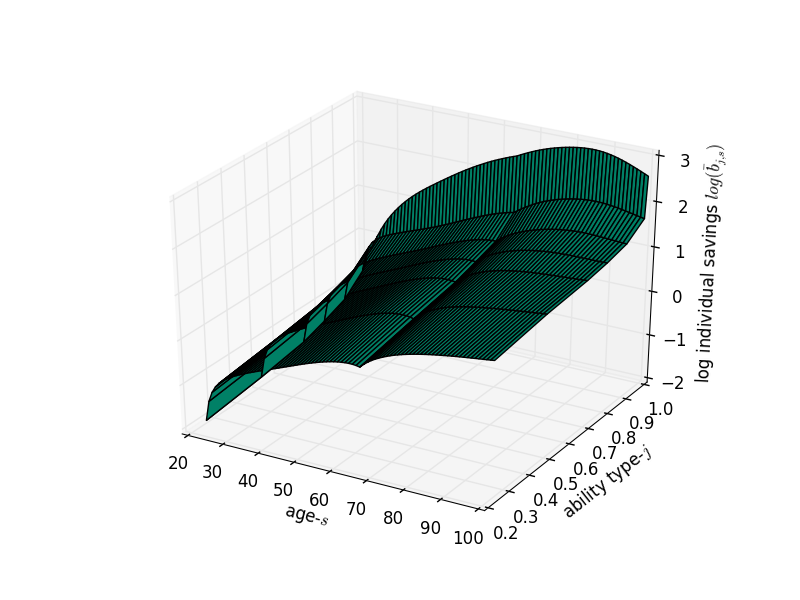
\includegraphics{images/SavSS_log.png}}}
%    \end{figure}
%
%    \begin{figure}[htb]\centering \captionsetup{width=4.0in}
%      \caption{\label{FigLabSS}\textbf{Stationary steady-state distribution of individual labor supply $\bar{n}_{j,s}$ for $S=80$ and $J=7$}}
%      \fbox{\resizebox{4.0in}{3.0in}{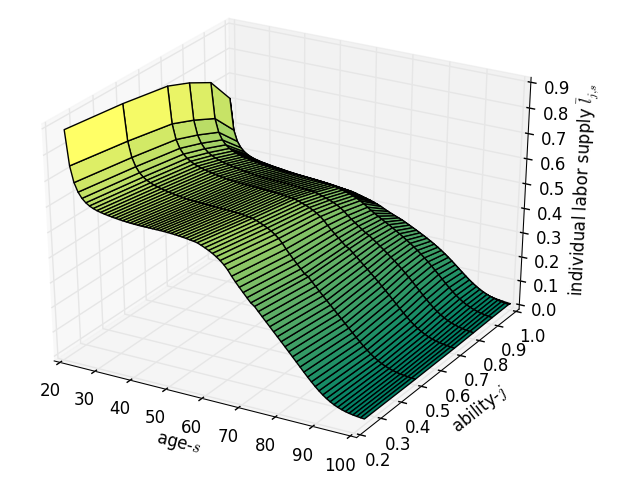
\includegraphics{images/LabSS.png}}}
%    \end{figure}
%
%    \begin{figure}[htb]\centering \captionsetup{width=4.0in}
%      \caption{\label{FigLogConsSS}\textbf{Stationary steady-state distribution of consumption $\bar{c}_{j,s}$ for $S=80$ and $J=7$}}
%      \fbox{\resizebox{4.0in}{3.0in}{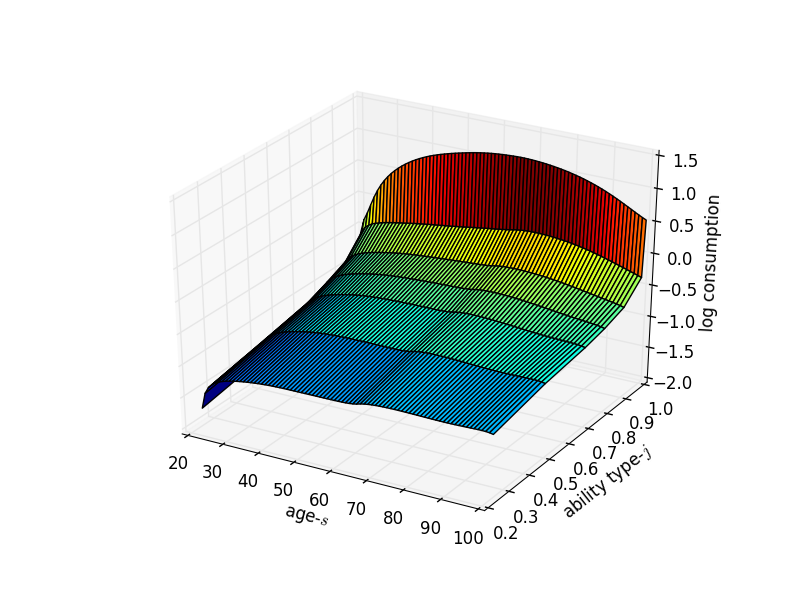
\includegraphics{images/ConsSS_log.png}}}
%    \end{figure}
%
%    Figure \ref{FigLogSavSS} shows the stationary steady-state distribution of individual savings $\bar{b}_{j,s}$ in logarithms, Figure \ref{FigLabSS} shows the stationary steady-state distribution of individual labor supply $\bar{n}_{j,s}$, and Figure \ref{FigLogConsSS} shows the steady-state distribution of consumption $\bar{c}_{j,s}$ in logarithms for a particular calibration of the model described in Table \ref{TabExogVars}. Notice from Figure \ref{FigLogConsSS} the hump-shaped pattern of consumption over the life cycle for each ability type, which is consistent with consumption data. Also note from the comparison of the distribution of savings in Figure \ref{FigLogSavSS} in comparison to the distribution of consumption in \ref{FigLogConsSS} that households use savings to smooth out consumption as much as possible, with a sharpe change in savings around retirement $s=R$ and only a small smooth lump in consumption at that age.

    The definition of the stationary non-steady-state equilibrium is similar to Definition \ref{DefEquilSS}, with the stationary steady-state equilibrium definition being a special case of the stationary non-steady-state equilibrium.

\ \\ 
WHAT FOLLOWS NEEDS UPDATING TO INCLUDE RICHER FIRM AND GOV'T, BUT IS HELPFUL IN SEEING THAT NON-SS EQ'M WILL LOOK LIKE...

\ \\

    \hrule
    \begin{definition}[\textbf{Stationary non-steady-state equilibrium}]\label{DefEquilNonSS}
      A non-autarkic stationary non-steady-state equilibrium in the overlapping generations model with $S$-period lived agents and heterogeneous ability $e_{j,s}$ is defined as allocations $n_{j,s,t}$ and $\hat{b}_{j,s+1,t+1}$ and prices $\hat{w}_t$ and $r_t$ for all $j$, $s$, and $t$ such that the following conditions hold:
       \begin{enumerate}
          \item households have symmetric beliefs $\Omega(\cdot)$ about the evolution of the distribution of savings, and those beliefs about the future distribution of savings equal the realized outcome (rational expectations),
            \begin{equation*}
              \bm{\hat{\Gamma}}_{t+u} = \bm{\hat{\Gamma}}^e_{t+u} = \Omega^u\left( \bm{\hat{\Gamma}}_t\right) \quad\forall t, \quad u\geq 1
            \end{equation*}
          \item households optimize according to \eqref{EqEulerLabStat}, \eqref{EqEulerSavStat}, and \eqref{EqEulerSavEpSstat}
          \item firms optimize according to \eqref{EqFOCwageStat} and \eqref{EqFOCrate}, and
          \item markets clear according to \eqref{EqMktClrLabStat} and \eqref{EqMktClrCapStat}.
       \end{enumerate}
    \end{definition}
    \hrule
   
   \ \\
   
    \noindent Taken together, the household labor-leisure and intended bequest decisions in the last period of life show that the optimal labor supply and optimal intended bequests for age $s=E+S$ are each functions of individual holdings of savings, total bequests received, and the prices in that period $n_{j,E+S,t}=\phi\bigl(\hat{b}_{j,E+S,t},\hat{BQ}_{j,t},\hat{w}_t,r_t\bigr)$ and $\hat{b}_{j,E+S+1,t+1}=\psi\bigl(\hat{b}_{j,E+S,t},\hat{BQ}_{j,t},\hat{w}_t,r_t\bigr)$. These two decisions are characterized by final-age version of the static labor supply Euler equation \eqref{EqEulerLabStat} and the static intended bequests Euler equation \eqref{EqEulerSavEpSstat}. Households in their second-to-last period of life in period $t$ have four decisions to make. They must choose how much to work this period $n_{j,E+S-1,t}$ and next period $n_{j,E+S,t+1}$, how much to save this period for next period $\hat{b}_{j,E+S,t+1}$, and how much to bequeath next period $\hat{b}_{j,E+S+1,t+2}$. The optimal responses for this individual are characterized by the $s=E+S-1$ and $s=E+S$ versions of the static Euler equations \eqref{EqEulerLabStat}, the $s=E+S-1$ version of the intertemporal Euler equation \eqref{EqEulerSavStat}, and the $s=E+S$ static bequest Euler equation \eqref{EqEulerSavEpSstat}, respectively.

    Optimal savings in the second-to-last period of life $s=E+S-1$ is a function of the current savings as well as the total bequests received and prices in the current period and in the next period $\hat{b}_{j,E+S,t+1} = \psi\bigl(\hat{b}_{j,E+S-1,t},\hat{BQ}_{j,t},\hat{w}_t,r_t,\hat{BQ}_{j,t+1},\hat{w}_{t+1},r_{t+1}|\Omega\bigr)$ given beliefs $\Omega$. As before, the optimal labor supply at age $s=E+S$ is a function of the next period's savings, bequests received, and prices $n_{j,E+S,t+1}=\phi\bigl(\hat{b}_{j,E+S,t+1},\hat{BQ}_{j,t+1},\hat{w}_{t+1},r_{t+1}\bigr)$. But the optimal labor supply at age $s=E+S-1$ is a function of the current savings, current bequests received, and the current prices as well as the future bequests received and future prices because of the dependence on the savings decision in that same period $n_{j,E+S-1,t}=\phi\bigl(\hat{b}_{j,E+S-1,t},\hat{BQ}_{j,t},\hat{w}_t,r_t,\hat{BQ}_{j,t+1},\hat{w}_{t+1},r_{t+1}|\Omega\bigr)$ given beliefs $\Omega$. By induction, we can show that the optimal labor supply, savings, and intended bequests functions for any individual with ability $j$, age $s$, and in period $t$ is a function of current holdings of savings and the lifetime path of total bequests received and prices given beliefs $\Omega$.
    \begin{align}
      n_{j,s,t} &= \phi\Bigl(\hat{b}_{j,s,t},\bigl(\hat{BQ}_{j,v},\hat{w}_v,r_v\bigr)_{v=t}^{t+S-s}|\Omega\Bigr) \quad\forall j,s,t \label{EqLabPolFuncGen} \\
      \hat{b}_{j,s+1,t+1} &= \psi\Bigl(\hat{b}_{j,s,t},\bigl(\hat{BQ}_{j,v},\hat{w}_v,r_v\bigr)_{v=t}^{t+S-s}|\Omega\Bigr) \quad\forall j,t \quad\text{and}\quad E+1\leq s\leq E+S \label{EqSavPolFuncGen}
    \end{align}

    If one knows the current distribution of households savings and intended bequests $\bm{\hat{\Gamma}}_t$ and has a beliefs function that predicts the law of motion over time for $\bm{\hat{\Gamma}}_t$, then one can predict time series for total bequests received $\hat{BQ}_{j,t}$, real wages $\hat{w}_t$ and real interest rates $r_t$ necessary for solving each household's optimal decisions. Characteristic (i) in equilibrium definition \ref{DefEquilNonSS} that individuals be able to forecast prices with perfect foresight over their lifetimes implies that each individual has correct information and beliefs about all the other individuals optimization problems and information. It also implies that the equilibrium allocations and prices are really just functions of the entire distribution of savings at a particular period, as well as a law of motion for that distribution of savings.

    In equilibrium, the steady-state household labor supplies $\bar{n}_{j,s}$ for all $j$ and $s$, the steady-state savings $\bar{b}_{j,E+S+1}$, the steady-state real wage $\bar{w}$, and the steady-state real rental rate $\bar{r}$ are simply functions of the steady-state distribution of savings $\bar{\Gamma}$. This is clear from the steady-state version of the capital market clearing condition \eqref{EqMktClrCapStat} and the fact that aggregate labor supply is a function of the sum of exogenous efficiency units of labor in the labor market clearing condition \eqref{EqMktClrLabStat}. And the two firm first order conditions for the real wage $\hat{w}_t$ \eqref{EqFOCwageStat} and real rental rate $r_t$ \eqref{EqFOCrate} are only functions of the stationary aggregate capital stock $\hat{K}_t$ and aggregate labor $\hat{L}_t$.

    \begin{figure}[htb]\centering \captionsetup{width=4.0in}
      \caption{\label{FigKpathTPI}\textbf{Equilibrium time path of $K_t$ for $S=80$ and $J=7$}}
      \fbox{\resizebox{4.0in}{3.0in}{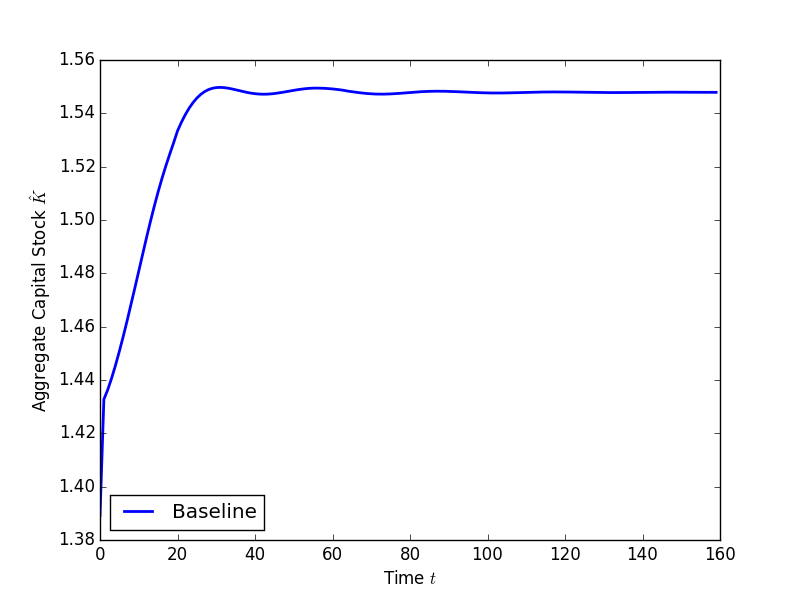
\includegraphics{images/KpathTPI.png}}}
    \end{figure}

    \begin{figure}[htb]\centering \captionsetup{width=4.0in}
      \caption{\label{FigLpathTPI}\textbf{Equilibrium time path of $L_t$ for $S=80$ and $J=7$}}
      \fbox{\resizebox{4.0in}{3.0in}{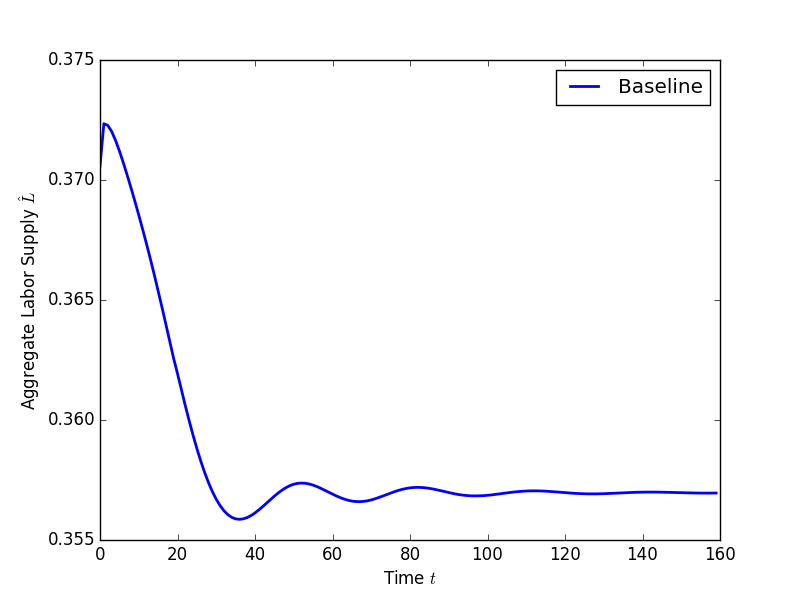
\includegraphics{images/LpathTPI.png}}}
    \end{figure}



\chapter{Numerical Solution}
\label{chap:model_soln}
\index{Numerical Solution%
@\emph{Numerical Solution}}%



%\pagestyle{empty}


When solving for the full transition path, we solve the model in two steps.  First, we solve for the steady state prices and allocations.  Next, we iterate backwards solving for prices and allocations along the transition path to the steady state.  Here we define the solution to the model, starting with the steady-state solution.


\section{Solving for stationary steady-state equilibrium}\label{AppSSsolve}

  This section describes the solution method for the stationary steady-state equilibrium described in Definition \ref{DefEquilSS}.  To obtain the steady-state equilibrium, we do the following:
  
 
   \begin{enumerate}
    \item Use the techniques in Chapter \ref{AppPopGrowth} to solve for the steady-state population distribution vector $\bm{\bar{\omega}}$ of the exogenous population process.
    \item Choose an initial guess for the stationary steady-state wage rate, $\bar{w}$ and real interest rate, $\bar{r}$.
%      \begin{itemize}
%        \item A good first guess is a large positive number for all the $\bar{n}_{j,s}$ that is slightly less than $\tilde{l}$ and to choose some small positive number for $\bar{b}_{j,s+1}$ that is small enough to be less than the minimum income that an individual might have $\bar{w}e_{j,s}\bar{n}_{j,s}$.
%      \end{itemize}
   \item With $\bar{w}$ and $\bar{r}$, use an unconstrained root finder to solve the $4\times 2 \times M$ equations defining the steady-state version of the firms' problem.  This will yield $\bar{I}_{m,c}$, $\bar{EL}_{m,c}$, $\bar{V}_{m,c}$, $\bar{p}_{m,c}$.
   \item Using $\bar{p}_{m,c}$ and the fixed coefficient matrix $\Pi$, we can determine $\bar{p}_{i}$, the price of consumption goods.
   \item $\bar{p}_{i}$ and maximization of the consumer's subutility function imply $\bar{p}_{s}$, the price of the composite consumption good.
    \item Perform an unconstrained root finder that chooses $\bar{c}_{j,s}$ and $\bar{b}_{j,s+1}$ that solves the $2JS$ stationary steady-state Euler equations.
    \item Make sure none of the implied steady-state consumptions $\bar{c}_{j,s}+\sum_{i=1}^{I}c_{i,s}$ exceeds income.
      \begin{itemize}
        \item If consumption exceeds income, the individual can not afford the minimum required consumption amounts.  We then...
      \end{itemize}
    \item Given consumption demand and the fixed coefficient matrix $\Xi$, find the implied demand for output, $X_{m}$.
    \item Use the consumer's subutility function over corporate and non-corporate goods to determine demand for corporate and non-corporate production goods to get $X_{m,n}$ and $X_{m,nc}$.
    \item Make sure that demand for these production goods matches the supply given firm's decisions in (iii).
    \item Make sure that none of the Euler errors is too large in absolute value for interior stationary steady-state values. A steady-state Euler error is the following, which is supposed to be close to zero for all $j$ and $s$:
      \begin{align}
        \begin{split}
          &\frac{\chi^n_{s}\left(\frac{b}{\tilde{l}}\right)\left(\frac{\bar{n}_{j,s}}{\tilde{l}}\right)^{v-1}\left[1 - \left(\frac{\bar{n}_{j,s}}{\tilde{l}}\right)\right]^{\frac{1-v}{v}}}{(\bar{c}_{j,s})^{-\sigma}\left(\bar{w} e_{j,s} - \frac{\partial\bar{T}_{j,s}}{\partial \bar{n}_{j,s}}\right)} - 1 \\
          &\qquad\qquad\qquad\qquad\qquad\qquad\qquad\forall j\quad\text{and}\quad E+1\leq s\leq E+S
        \end{split} \label{EqSSeulerrLab} \\
        \begin{split}
          &\frac{e^{-g_y\sigma}\left(\rho_s\chi^b \left(\bar{b}_{j,s+1}\right)^{-\sigma} + \beta(1-\rho_s)(\bar{c}_{j,s+1})^{-\sigma}\left[(1 + \bar{r}) - \frac{\partial \bar{T}_{j,s+1}}{\partial \bar{b}_{j,s+1}}\right]\right)}{(\bar{c}_{j,s})^{-\sigma}} - 1 \\
          &\qquad\qquad\qquad\qquad\qquad\qquad\qquad\forall j \quad\text{and}\quad E+1\leq s\leq E+S-1 \\
        \end{split} \label{EqSSeulerrSav} \\
        &\frac{\chi^b e^{-g_y\sigma}(\bar{b}_{j,E+S+1})^{-\sigma}}{\left(\bar{c}_{j,E+S}\right)^{-\sigma}} - 1 \quad\forall j \label{EqSSeulerrBeq}
      \end{align}
  \end{enumerate}
  
   

%FIRMS STUFF:
%\section{Solving the model}
%
%
%\subsection{Solving for the steady state}
%
%On the supply side (with one sector), we have to solve for the factor prices, $\bar{i}$ and $bar{w}$ (the price of output $\bar{p}^{C}$ is normalized to one), the shadow price of capital, $\bar{q}^{C}$, and the allocations $\bar{EL}^{C}$, $\bar{K}^{C}$, $\bar{I}^{C}$.  From these all the other variables follow trivially.  
%
%Start by solving for the steady-states of Equations \ref{eqn:opt_i} and \ref{eqn:foc_k}.  Equation \ref{eqn:opt_i} becomes:
%
%\begin{equation}
%\label{eqn:opt_i_ss}
%\bar{q}^{C}=\underbrace{1-b^{C}-\bar{\Omega}^{C}\bar{\tau}^{b}(f_{e}-f_{b}b^{C})-f_{d}(1-f_{e})\bar{Z}^{C}}_{\text{function of only parameters}}
%\end{equation}
%
%This yields the solution to $\bar{q}^{C}$.
%
%Next, consider the steady-state of Equation \ref{eqn:foc_k}:
%
%\begin{equation}
%\label{eqn:foc_k_ss}
%\bar{q}^{C}=\frac{1}{1+\bar{\theta}}\left[(1-\delta^{C})\bar{q}^{C} + \frac{\partial \bar{X}^{C}}{\partial \bar{K}^{C}} - \{(1-\bar{\tau}^{b})\bar{\Omega}^{C}\bar{\tau}^{pC} + (1-f_{i}\bar{\tau}^{i})\bar{i}\bar{\Omega}^{C}b^{C} - \delta^{C}(1-b^{C}-\bar{\Omega}^{C}(1-f_{p}\bar{\tau}^{b}b^{C}))\}\right]
%\end{equation}
%
%We can rearrange this and solve for the steady-state marginal product of capital in sector $C$:
%
%\begin{equation}
%\label{eqn:mpk_ss}
%\frac{\partial \bar{X}^{C}}{\partial \bar{K}^{C}} = (\bar{\theta}+\delta^{C})\bar{q}^{C} + (1-\bar{\tau}^{b})\bar{\Omega}^{C}\bar{\tau}^{pC} + (1-f_{i}\bar{\tau}^{i})\bar{i}\bar{\Omega}^{C}b^{C} - \delta^{C}(1-b^{C}-\bar{\Omega}^{C}(1-f_{p}\bar{\tau}^{b}b^{C}))
%\end{equation}
%
%Notice that given Equation \ref{eqn:opt_i_ss}, the RHS to the above equation is function of parameters and the steady state nominal interest rate, $\bar{i}$.  The LHS of the equation is a function of $\bar{K}^{C}$ and $\bar{EL}^{C}$.
%
%I think we can use the following to identify the SS values of the variables of interest:
%\begin{enumerate}
%\item $\bar{i}$ will be determined by the SS of the household's Euler equations (I think this can be done as described in the HH sol'n method)
%\item $\bar{w}$ will be determined by the SS of the household's FOCs for labor supply ((I think this can be done as described in the HH sol'n method)
%\item $\bar{q}^{C}$ is determined by Equation \ref{eqn:opt_i_ss}
%\item $\bar{EL}^{C}$ is determined by the SS version of Equation \ref{eqn:foc_l}, plus $\bar{w}$
%\item $\bar{K}^{C}$ is determined by Equation \ref{eqn:mpk_ss} and $\bar{i}$
%\item $\bar{I}^{C}$ is then solved for using the steady state law of motion for capital $\implies \bar{I}^{C}=\delta^{C}\bar{K}^{C}$
%\end{enumerate}
%
%In solving for $\bar{EL}^{C}$ and $\bar{K}^{C}$, note that we'll have use the MPK and the MPL simultaneously.  Given our production function, we have:
%
%\begin{equation}
%\label{eqn:mpk}
%\frac{\partial X^{C}_{u}}{\partial K^{C}_{u}} = \left[(\gamma_{C})^{1/\epsilon_{C}}(K^{C}_{u})^{(\epsilon_{C}-1)/\epsilon_{C}}+(1-\gamma_{C})^{1/\epsilon_{C}}(EL^{C}_{u})^{(\epsilon_{C}-1)/\epsilon_{C}}\right]^{1/(\epsilon_{C}-1)}(\gamma_{C})^{1/\epsilon_{C}}(K^{C}_{u})^{-1/\epsilon_{C}}
%\end{equation}
%
%and 
%
%\begin{equation}
%\label{eqn:mpl}
%\frac{\partial X^{C}_{u}}{\partial EL^{C}_{u}} = \left[(\gamma_{C})^{1/\epsilon_{C}}(K^{C}_{u})^{(\epsilon_{C}-1)/\epsilon_{C}}+(1-\gamma_{C})^{1/\epsilon_{C}}(EL^{C}_{u})^{(\epsilon_{C}-1)/\epsilon_{C}}\right]^{1/(\epsilon_{C}-1)}(1-\gamma_{C})^{1/\epsilon_{C}}(EL^{C}_{u})^{-1/\epsilon_{C}}
%\end{equation}
%
%We know that, at an optimum, the marginal revenue product of labor equals the wage rate, and the marginal revenue product of capital equals a function of the interest rate, marginal $q$, and the model parameters.  Call this function $g(i_{u},q^{C}_{u},q^{C}_{u-1},\Theta)$.  We thus have $p^{C}_{u}\frac{\partial X^{C}_{u}}{\partial EL^{C}_{u}} =w_{u}$ and $p^{C}_{u}\frac{\partial X^{C}_{u}}{\partial K^{C}_{u}}=g(i_{u},q^{C}_{u},q^{C}_{u-1},\Theta)$.  Dividing these two equations, we have:
%
%\begin{equation}
%\label{eqn:cap_lab_ratio}
%\begin{split}
%& \frac{\frac{\partial X^{C}_{u}}{\partial K^{C}_{u}}}{\frac{\partial X^{C}_{u}}{\partial EL^{C}_{u}}} =\frac{(\gamma_{C})^{1/\epsilon_{C}}(K^{C}_{u})^{-1/\epsilon_{C}}}{(1-\gamma_{C})^{1/\epsilon_{C}}(EL^{C}_{u})^{-1/\epsilon_{C}}}-=\frac{g(i_{u},q^{C}_{u},q^{C}_{u-1},\Theta)}{w_{u}} \\
%& \implies \frac{K^{C}_{u}}{EL^{C}_{u}} =\frac{(1-\gamma_{C})}{\gamma_{C}}\left(\frac{w_{u}} {g(i_{u},q^{C}_{u},q^{C}_{u-1},\Theta)}\right)^{\epsilon_{C}} \\
%\end{split}
%\end{equation}
%
%We can use the SS version of Equation \ref{eqn:cap_lab_ratio} to solve for capital as function of labor (and $\bar{q}, \bar{i}, \bar{w}$), and then use that in the SS version of Equation \ref{eqn:mpl} to solve for labor as s function of $\bar{q}, \bar{i}, \bar{w}$.  We then go back to the SS version of Equation \ref{eqn:cap_lab_ratio} to get the SS choice of capital as a function of $\bar{q}, \bar{i}, \bar{w}$.
%
%All of the above will work for each sector in a model with any number of sectors (though care has to be taken to include the prices of output and capital in those other sectors, since only one sector's output can be the numeraire).
%
%\subsection{Solving for the transition path}
%
%I believe we can just use the Euler equations to go backwards in time, from the SS back along the transition path to $t=0$.  Assume period $T$ is the SS,  The solution would look like the following:
%
%\begin{enumerate}
%\item Use Equation \ref{eqn:foc_k} to solve for the for $q^{C}_{T-1}$ since we have the solution to the RHS of the equation after we've solved for the SS.
%\item Use the law of motion for capital to find: $K^{C}_{T-1}=\frac{K^{C}_{T}-I^{C}_{T-1}}{(1-\delta^{C})}=\frac{\bar{K}^{C}-I^{C}_{T-1}}{(1-\delta^{C})}$
%\item Use Equation \ref{eqn:opt_i} and the value of $q^{C}_{T-1}$ to find $I^{C}_{T-1}$ (and $K^{C}_{T-1}$ given the law of motion relationship.
%\item Given $w_{T-1}$ we can use the FOC for labor demand to find $EL^{C}_{T-1}$
%\item Given $i_{T-1}$ we can use Equation \ref{eqn:foc_k} to solve for $q^{C}_{T-2}$ 
%\item We then repeat the above steps until we work back to $t=0$.
%\end{enumerate}
%
%
%
%To solve for any stationary non-steady-state equilibrium time path of the economy from an arbitrary current state to the steady state, we follow the time path iteration (TPI) method of \citet{AuerbachKotlikoff:1987}. Appendix \ref{AppNonSSsolve} details how to solve for the non-steady-state equilibrium time path using the TPI method. The approach is to choose an arbitrary time path for the stationary aggregate capital stock $\hat{K}_t$, stationary aggregate labor $\hat{L}_t$, and total bequests received $\hat{BQ}_{j,t}$ for each type $j$. This initial guess of a path implies arbitrary beliefs that violate the rational expectations requirement. We then solve for households' optimal decisions given the time paths of those variables, which decisions imply new time paths of those variables. We then update the time path as a convex combination of the initial guess and the new implied path. Figure \ref{FigKpathTPI} shows the equilibrium time path of the aggregate capital stock for the calibration described in Table \ref{TabExogVars} for $T=160$ periods starting from an initial distribution of savings in which $b_{j,s,1}=\bm{\bar{\Gamma}}$ for all $j$ and $s$ in the case that no policy experiment takes place. The initial capital stock $\hat{K}_1$ is not at the steady state $\bar{K}$ because the initial population distribution is not at the steady-state.
%
%
%
%

\section{Solving for stationary non-steady-state equilibrium by time path iteration}\label{AppNonSSsolve}

  \setcounter{equation}{0}

  This section outlines the benchmark time path iteration (TPI) method of \citet{AuerbachKotlikoff:1987} for solving the stationary non-steady-state equilibrium transition path of the distribution of savings. TPI finds a fixed point for the transition path of the distribution of capital for a given initial state of the distribution of capital. The idea is that the economy is infinitely lived, even though the agents that make up the economy are not. Rather than recursively solving for equilibrium policy functions by iterating on individual value functions, one must recursively solve for the policy functions by iterating on the entire transition path of the endogenous objects in the economy (see \citet[ch. 17]{StokeyLucas:1989}).

  The key assumption is that the economy will reach the steady-state equilibrium described in Definition \ref{DefEquilSS} in a finite number of periods $T<\infty$ regardless of the initial state. Let $\bm{\hat{\Gamma}}_t$ represent the distribution of stationary savings at time $t$.
  \begin{equation}\tag{\ref{EqSavDist}}
    \bm{\hat{\Gamma}}_t \equiv \Bigl\{\bigl\{\hat{b}_{j,s,t}\bigr\}_{j=1}^J\Bigr\}_{s=E+2}^{E+S+1}, \quad\forall t
  \end{equation}
  In Section \ref{SecMCEqlbm}, we describe how the stationary non-steady-state equilibrium time path of allocations and price is described by functions of the state $\bm{\hat{\Gamma}}_t$ and its law of motion. TPI starts the economy at any initial distribution of savings $\bm{\hat{\Gamma}}_1$ and solves for its equilibrium time path over $T$ periods to the steady-state distribution $\bm{\bar{\Gamma}}_T$.

  The first step is to assume an initial transition path for aggregate stationary capital $\bm{\hat{K}}^i = \left\{\hat{K}_1^i,\hat{K}_2^i,...\hat{K}_T^i\right\}$, aggregate stationary labor $\bm{\hat{L}}^i = \left\{\hat{L}_1^i,\hat{L}_2^i,...\hat{L}_T^i\right\}$, and total bequests received $\bm{\hat{BQ}}_j^i=\{\hat{BQ}_{j,1}^i,\hat{BQ}_{j,2}^i,...\hat{BQ}_{j,T}^i\}$ for each ability type $j$ such that $T$ is sufficiently large to ensure that $\bm{\hat{\Gamma}}_T = \bar{\bm{\Gamma}}$, $\hat{K}_T^i\left(\bm{\Gamma}_T\right)$, $\hat{L}_T^i\left(\bm{\Gamma}_T\right) = \bar{L}\left(\bar{\bm{\Gamma}}\right)$, and $\hat{BQ}_{j,T}^i\left(\bm{\Gamma}_T\right) = \bar{BQ}_j\left(\bar{\bm{\Gamma}}\right)$ for all $t\geq T$. The superscript $i$ is an index for the iteration number. The transition paths for aggregate capital and aggregate labor determine the transition paths for both the real wage $\bm{\hat{w}}^i = \left\{\hat{w}_1^i,\hat{w}_2^i,...\hat{w}_T^i\right\}$ and the real return on investment $\bm{r}^i = \left\{r_1^i,r_2^i,...r_T^i\right\}$. The time paths for the total bequests received also figure in each period's budget constraint and are determined by the distribution of savings and intended bequests.

  The exact initial distribution of capital in the first period $\bm{\hat{\Gamma}}_1$ can be arbitrarily chosen as long as it satisfies the stationary capital market clearing condition \eqref{EqMktClrCapStat}.
  \begin{equation}\label{EqMktClrCapStat1}
    \hat{K}_1 = \frac{1}{1 + \tilde{g}_{n,1}}\sum_{s=E+2}^{E+S+1}\sum_{j=1}^{J}\hat{\omega}_{s-1,0}\lambda_j \hat{b}_{j,s,1}
  \end{equation}
  Simiilarly, each initial value of total bequests received $\hat{BQ}_{j,1}^i$ must be consistent with the initial distribution of capital through the stationary version of \eqref{EqTotBeq}.
  \begin{equation}\label{EqTotBeqStat1}
    \hat{BQ}_{j,1} = \frac{(1+r_1)\lambda_j}{1+\tilde{g}_{n,1}}\sum_{s=E+1}^{E+S}\rho_s\hat{\omega}_{s,0}\hat{b}_{j,s+1,1} \quad\forall j
  \end{equation}
  However, this is not the case with $\hat{L}_1^i$. Its value will be endogenously determined in the same way the $K_2^i$ is. For this reason, a logical initial guess for the time path of aggregate labor is the steady state in every period $L_t^1 = \bar{L}$ for all $1\leq t\leq T$.

  It is easiest to first choose the initial distribution of savings $\bm{\hat{\Gamma}}_1$ and then choose an initial aggregate capital stock $\hat{K}_1^i$ and initial total bequests received $\hat{BQ}_{j,1}^i$ that correspond to that distribution. As mentioned earlier, the only other restrictions on the initial transition paths for aggregate capital, aggregate labor, and total bequests received is that they equal their steady-state levels $\hat{K}_T^i = \bar{K}\left(\bm{\bar{\Gamma}}\right)$, $\hat{L}_T^i = \bar{L}\left(\bm{\bar{\Gamma}}\right)$, and $\hat{BQ}_{j,T}^i = \bar{BQ}_j\left(\bm{\bar{\Gamma}}\right)$ by period $T$. \citet{EvansPhillips:2014} have shown that the initial guess for the aggregate capital stocks $\hat{K}_t^i$ for periods $1<t<T$ can take on almost any positive values satisfying the constraints above and still have the time path iteration converge.

  Given the initial savings distribution $\bm{\hat{\Gamma}}_1$ and the transition paths of aggregate capital $\bm{\hat{K}}^i = \left\{\hat{K}_1^i,\hat{K}_2^i,...\hat{K}_T^i\right\}$, aggregate labor $\bm{\hat{L}}^i = \left\{\hat{L}_1^i,\hat{L}_2^i,...\hat{L}_T^i\right\}$, and total bequests received $\bm{\hat{BQ}}_j^i = \left\{\hat{BQ}_{j,1}^i,\hat{BQ}_{j,2}^i,...\hat{BQ}_{j,T}^i\right\}$, as well as the resulting real wage $\bm{\hat{w}}^i = \left\{\hat{w}_1^i,\hat{w}_2^i,...\hat{w}_T^i\right\}$, and real return to savings $\bm{r}^i = \left\{r_1^i,r_2^i,...r_T^i\right\}$, one can solve for the period-1 optimal labor supply and intended bequests for each type $j$ of $s=E+S$-aged agents in the last period of their lives $n_{j,E+S,1}=\phi_{j,E+S}(\hat{b}_{j,E+S,1},\hat{BQ}_{j,E+S,1},\hat{w}_1,r_1)$ and $\hat{b}_{j,E+S+1,2}=\psi_{j,E+S}(\hat{b}_{j,E+S,1},\hat{BQ}_{j,E+S,1},\hat{w}_1,r_1)$ using his two $s=E+S$ static Euler equations \eqref{EqEulerLabStat} and \eqref{EqEulerSavEpSstat}.
  \begin{equation}\label{EqEulerSlabt1}
    \begin{split}
      &(\hat{c}_{j,E+S,1})^{-\sigma}\Biggl(\hat{w}_1^i e_{j,E+S} - \frac{\partial\hat{T}_{j,E+S,1}}{\partial n_{j,E+S,1}}\Biggr) = ... \\
      &\qquad\qquad\qquad\qquad \chi^n_{E+S}\biggl(\frac{b}{\tilde{l}}\biggr)\biggl(\frac{n_{j,E+S,1}}{\tilde{l}}\biggr)^{v-1}\Biggl[1 - \biggl(\frac{n_{j,E+S,1}}{\tilde{l}}\biggr)\Biggr]^{\frac{1-v}{v}} \quad\forall j \\
      &\quad\text{where}\quad \hat{c}_{j,E+S,1} = ... \\
      &\qquad\qquad\qquad \left(1 + r_1^i\right)\hat{b}_{j,E+S,1} + \hat{w}_1^i e_{j,E+S}n_{j,E+S,1} + \frac{\hat{BQ}_{j,1}}{\lambda_j} - e^{g_y}\hat{b}_{j,E+S+1,2} - \hat{T}_{j,E+S,1} \\
      &\quad\text{and}\quad \frac{\partial \hat{T}_{j,E+S,1}}{\partial n_{j,E+S,1}} = ... \\
      &\qquad\qquad\qquad \hat{w}_1^i e_{j,E+S}\biggl[\tau^I\bigl(F\hat{a}_{j,E+S,1}\bigr) + \frac{\hat{a}_{j,E+S,1}CDF\bigl[2A(F\hat{a}_{j,E+S,1})+B\bigr]}{\bigl[A(F\hat{a}_{j,E+S,1})^2+B(F \hat{a}_{j,E+S,1})+C\bigr]^2} + \tau^P\Biggr]
    \end{split}
  \end{equation}
  \begin{equation}\label{EqEulerSbeqt1}
    (\hat{c}_{j,E+S,1})^{-\sigma} = \chi^b e^{-g_y\sigma}(\hat{b}_{j,E+S+1,2})^{-\sigma} \quad\forall j
  \end{equation}
  Note that this is simply two equations \eqref{EqEulerSlabt1} and \eqref{EqEulerSbeqt1} and two unknowns $n_{j,E+S,1}$ and $\hat{b}_{j,E+S+1,2}$.

  We then solve the problem for all $j$ types of $E+S-1$-aged individuals in period $t=1$, each of which entails labor supply decisions in the current period $n_{j,E+S-1,1}$ and in the next period $n_{j,E+S,2}$, a savings decision in the current period for the next period $\hat{b}_{j,E+S,2}$ and an intended bequest decision in the last period $\hat{b}_{j,E+S+1,3}$. The labor supply decision in the initial period and the savings period in the initial period for the next period for each type $j$ of $E+S-1$-aged individuals are policy functions of the current savings and the total bequests received and prices in this period and the next $\hat{b}_{j,E+S,2} = \psi_{j,E+S-1}(\hat{b}_{j,E+S-1,1},\{\hat{BQ}_{j,t},\hat{w}_t,r_t\}_{t=1}^2)$ and $\hat{n}_{j,E+S-1,1} = \phi_{j,E+S-1}(\hat{b}_{j,E+S-1,1},\{\hat{BQ}_{j,t},\hat{w}_t,r_t\}_{t=1}^2)$. The labor supply and intended bequests decisions in the next period are simply functions of the savings, total bequests received, and prices in that period $\hat{n}_{j,E+S,2} = \phi_{j,E+S}(\hat{b}_{j,E+S,2},\hat{BQ}_{j,2},\hat{w}_2,r_2)$ and $\hat{b}_{j,E+S+1,3} = \psi_{j,E+S}(\hat{b}_{j,E+S,2},\hat{BQ}_{j,2},\hat{w}_2,r_2)$. These four functions are characterized by the following versions of equations \eqref{EqEulerLabStat}, \eqref{EqEulerSavStat}, and \eqref{EqEulerSavEpSstat}.
  \begin{equation}\label{EqEulerSm1labt1}
    \begin{split}
      &(\hat{c}_{j,E+S-1,1})^{-\sigma}\Biggl(\hat{w}_1^i e_{j,E+S-1} - \frac{\partial\hat{T}_{j,E+S-1,1}}{\partial n_{j,E+S-1,1}}\Biggr) = ... \\
      &\qquad\qquad\qquad \chi^n_{E+S-1}\biggl(\frac{b}{\tilde{l}}\biggr)\biggl(\frac{n_{j,E+S-1,1}}{\tilde{l}}\biggr)^{v-1}\Biggl[1 - \biggl(\frac{n_{j,E+S-1,1}}{\tilde{l}}\biggr)\Biggr]^{\frac{1-v}{v}} \quad\forall j
    \end{split}
  \end{equation}
  \begin{equation}\label{EqEulerSm1savt1}
    \begin{split}
      &(\hat{c}_{j,E+S-1,1})^{-\sigma} = ... \\
      &e^{-g_y\sigma}\Biggl(\rho_{E+S-1}\chi^b \bigl(\hat{b}_{j,E+S,2}\bigr)^{-\sigma} + \beta(1-\rho_{E+S-1})(\hat{c}_{j,E+S,2})^{-\sigma}\Biggl[(1 + r_2^i) - \frac{\partial T_{j,E+S,2}}{\partial b_{j,E+S,2}}\Biggr]\Biggr) \\
      &\qquad\qquad\qquad\qquad\qquad\qquad\qquad\qquad\qquad\qquad\qquad\qquad\qquad\qquad\qquad\qquad\forall j \\
      &\qquad\text{where}\quad \frac{\partial T_{j,E+S,2}}{\partial b_{j,E+S,2}} = ...\\
      &\qquad\qquad r_2^i\Biggl(\tau^I(F\hat{a}_{j,E+S,2}) + \frac{F\hat{a}_{j,E+S,2}CD\left[2A(F\hat{a}_{j,E+S,2}) + B\right]}{\left[A(F\hat{a}_{j,E+S,2})^2 + B(F\hat{a}_{j,E+S,2}) + C\right]^2}\Biggr) ... \\
      &\qquad\qquad \tau^W(\hat{b}_{j,E+S,2}) + \frac{\hat{b}_{j,E+S,2}PHM}{\left(H\hat{b}_{j,E+S,2} + M\right)^2}
    \end{split}
  \end{equation}
  \begin{equation}\label{EqEulerSlabt2}
    \begin{split}
      &(\hat{c}_{j,E+S,2})^{-\sigma}\Biggl(\hat{w}_2^i e_{j,E+S} - \frac{\partial\hat{T}_{j,E+S,2}}{\partial n_{j,E+S,2}}\Biggr) = ... \\
      &\qquad\qquad\qquad \chi^n_{E+S}\biggl(\frac{b}{\tilde{l}}\biggr)\biggl(\frac{n_{j,E+S,2}}{\tilde{l}}\biggr)^{v-1}\Biggl[1 - \biggl(\frac{n_{j,E+S,2}}{\tilde{l}}\biggr)\Biggr]^{\frac{1-v}{v}} \quad\forall j
    \end{split}
  \end{equation}
  \begin{equation}\label{EqEulerSsavt2}
    (\hat{c}_{j,E+S,2})^{-\sigma} = \chi^b e^{-g_y\sigma}(\hat{b}_{j,E+S+1,3})^{-\sigma} \quad\forall j
  \end{equation}
  Note that this is four equations \eqref{EqEulerSm1labt1}, \eqref{EqEulerSm1savt1}, \eqref{EqEulerSlabt2}, and \eqref{EqEulerSsavt2} and four unknowns $n_{j,E+S-1,1}$, $\hat{b}_{j,E+S,2}$, $n_{j,E+S,2}$, and $\hat{b}_{j,E+S+1,3}$.

  This process is repeated for every age of household alive in $t=1$ down to the age $s=E+1$ household at time $t=1$. Each of these households $j$ solves the full set of remaining $S-s+1$ labor supply decisions, $S-s$ savings decisions, and one intended bequest decision at the end of life. After the full set of lifetime decisions has been solved for all the households alive at time $t=1$, each ability $j$ household born in period $t\geq 2$ can be solved for, the solution to which is characterized by the following full set of Euler equations analogous to \eqref{EqEulerLabStat}, \eqref{EqEulerSavStat}, and \eqref{EqEulerSavEpSstat}.
  \begin{equation}\label{EqEulerslabt}
    \begin{split}
      &(\hat{c}_{j,s,t})^{-\sigma}\Biggl(\hat{w}_t^i e_{j,s} - \frac{\partial\hat{T}_{j,s,t}}{\partial n_{j,s,t}}\Biggr) =  \chi^n_{s}\biggl(\frac{b}{\tilde{l}}\biggr)\biggl(\frac{n_{j,s,t}}{\tilde{l}}\biggr)^{v-1}\Biggl[1 - \biggl(\frac{n_{j,s,t}}{\tilde{l}}\biggr)\Biggr]^{\frac{1-v}{v}} \\
      &\qquad\qquad\qquad\qquad\qquad\forall j \quad\text{and}\quad E+1\leq s\leq E+S\quad\text{and}\quad t\geq 2
    \end{split}
  \end{equation}

  \begin{equation}\label{EqEulersSavt}
    \begin{split}
      &(\hat{c}_{j,s,t})^{-\sigma} = ... \\
      &e^{-g_y\sigma}\Biggl(\rho_{s}\chi^b \bigl(\hat{b}_{j,s+1,t+1}\bigr)^{-\sigma} + \beta(1-\rho_{s})(\hat{c}_{j,s+1,t+1})^{-\sigma}\Biggl[(1 + r_{t+1}^i) - \frac{\partial T_{j,s+1,t+1}}{\partial b_{j,s+1,t+1}}\Biggr]\Biggr) \\
      &\qquad\qquad\qquad\forall j \quad\text{and}\quad E+1\leq s\leq E+S-1 \quad\text{and}\quad t\geq 2
    \end{split}
  \end{equation}

  \begin{equation}\label{EqEulerSsavt}
    (\hat{c}_{j,E+S,t})^{-\sigma} = \chi^b e^{-g_y\sigma}(\hat{b}_{j,E+S+1,t+1})^{-\sigma} \quad\forall j \quad\text{and}\quad t\geq 2
  \end{equation}
  For each household of ability type $j$ entering the economy in period $t\geq 1$, the entire set of $2S$ lifetime decisions is characterized by the $2S$ equations represented in \eqref{EqEulerslabt}, \eqref{EqEulersSavt}, and \eqref{EqEulerSsavt}.

  We can then solve for the entire lifetime of savings and labor supply decisions for each age $s=1$ individual in periods $t=2,3,...T$. The central part of the schematic diagram in Figure \ref{FigTPIdiag} shows how this process is done in order to solve for the equilibrium time path of the economy from period $t=1$ to $T$. Note that for each full lifetime savings and labor supply path solved for an individual born in period $t\geq 2$, we can solve for the aggregate capital stock and total bequests received implied by those savings decisions $\bm{\hat{K}}^{i'}$ and $\bm{\hat{BQ}}_{j}^{i'}$ and aggregate labor implied by those labor supply decisions $\bm{\hat{L}}^{i'}$.

  \begin{figure}[p]\centering \captionsetup{width=4.0in}
    \caption{\label{FigTPIdiag}\textbf{Diagram of TPI solution method within each iteration for $S=4$ and $J=1$}}
    \fbox{\resizebox{4.2in}{6.0in}{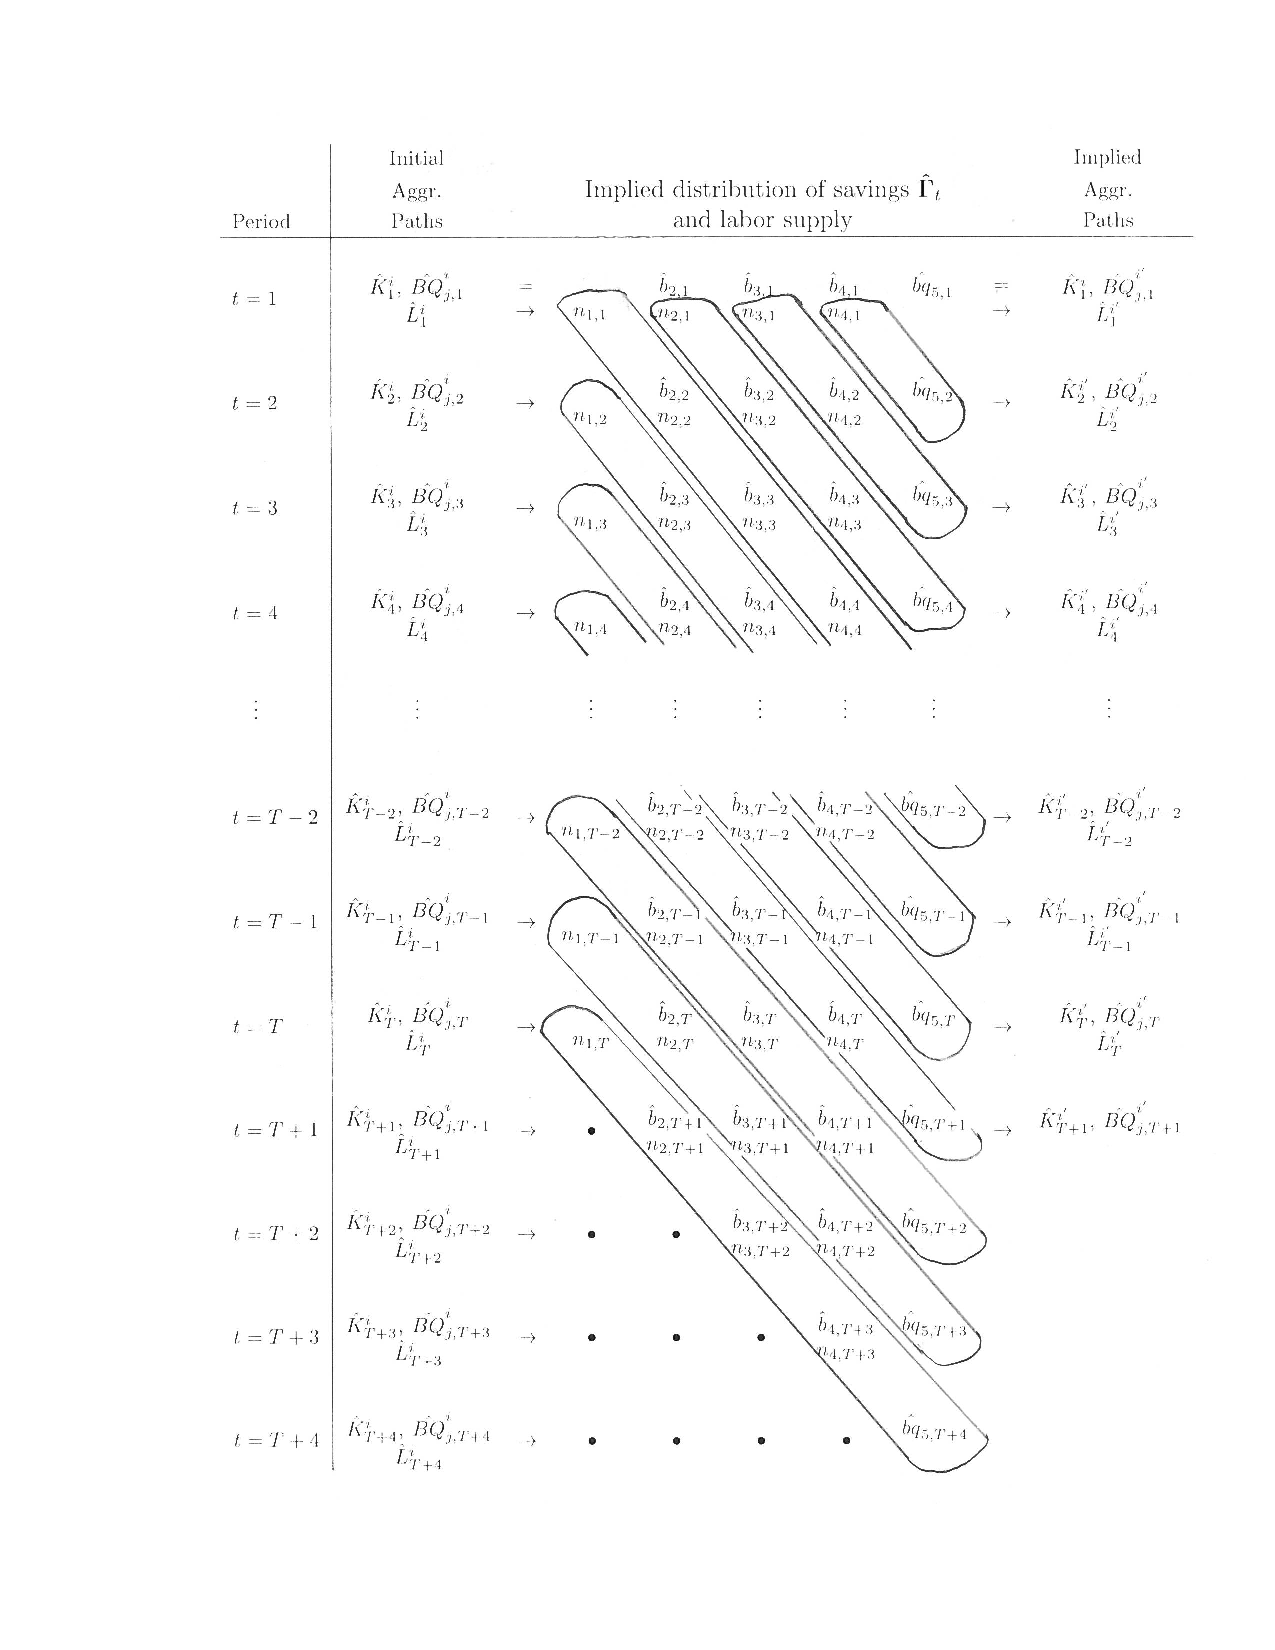
\includegraphics{images/TPIdiag.pdf}}}
  \end{figure}


  % THIS IS THE CODE FOR THE TABLE UNDERLYING THE FIGURE ABOVE
  % \begin{tabular}{>{\footnotesize}l| >{\footnotesize}c >{\footnotesize}c >{\footnotesize}c >{\footnotesize}c >{\footnotesize}c >{\footnotesize}c >{\footnotesize}c >{\footnotesize}c >{\footnotesize}c}
  %          & Initial & & & & & & & & Implied \\
  %          & Aggr. & & \multicolumn{5}{c}{Implied distribution of savings $\bm{\hat{\Gamma}}_t$} & & Aggr. \\
  %   Period & Paths    & & \multicolumn{5}{c}{and labor supply}   & & Paths    \\
  %   \hline
  %   & & & & & & & & & \\
  %   $t=1$ & $\begin{matrix}\hat{K}_1^i, \: \hat{BQ}_{j,1}^i \\ \hat{L}_1^i\end{matrix}$ & $\begin{matrix}= \\ \rightarrow\end{matrix}$ & $\begin{matrix}\: \\ n_{1,1}\end{matrix}$ & $\begin{matrix}\hat{b}_{2,1} \\ n_{2,1}\end{matrix}$ & $\begin{matrix}\hat{b}_{3,1} \\ n_{3,1}\end{matrix}$ & $\begin{matrix}\hat{b}_{4,1} \\ n_{4,1}\end{matrix}$ & $\begin{matrix}\hat{bq}_{5,1} \\ \,\end{matrix}$ & $\begin{matrix}= \\ \rightarrow\end{matrix}$ & $\begin{matrix}\hat{K}_1^i, \: \hat{BQ}_{j,1}^{i'} \\ \hat{L}^{i'}_1\end{matrix}$ \\[10mm]
  %   $t=2$ & $\begin{matrix}\hat{K}_2^i, \: \hat{BQ}_{j,2}^i \\ \hat{L}^i_2\end{matrix}$ & $\rightarrow$ & $\begin{matrix}\: \\ n_{1,2}\end{matrix}$ & $\begin{matrix}\hat{b}_{2,2} \\ n_{2,2}\end{matrix}$ & $\begin{matrix}\hat{b}_{3,2} \\ n_{3,2}\end{matrix}$ & $\begin{matrix}\hat{b}_{4,2} \\ n_{4,2}\end{matrix}$ & $\begin{matrix}\hat{bq}_{5,2} \\ \,\end{matrix}$ & $\rightarrow$ & $\begin{matrix}\hat{K}_2^{i'}, \: \hat{BQ}_{j,2}^{i'} \\ \hat{L}^{i'}_2\end{matrix}$ \\[10mm]
  %   $t=3$ & $\begin{matrix}\hat{K}_3^i, \: \hat{BQ}_{j,3}^i \\ \hat{L}^i_3\end{matrix}$ & $\rightarrow$ & $\begin{matrix}\: \\ n_{1,3}\end{matrix}$ & $\begin{matrix}\hat{b}_{2,3} \\ n_{2,3}\end{matrix}$ & $\begin{matrix}\hat{b}_{3,3} \\ n_{3,3}\end{matrix}$ & $\begin{matrix}\hat{b}_{4,3} \\ n_{4,3}\end{matrix}$ & $\begin{matrix}\hat{bq}_{5,3} \\ \,\end{matrix}$ & $\rightarrow$ & $\begin{matrix}\hat{K}_3^{i'}, \: \hat{BQ}_{j,3}^{i'} \\ \hat{L}^{i'}_3\end{matrix}$ \\[10mm]
  %   $t=4$ & $\begin{matrix}\hat{K}_4^i, \: \hat{BQ}_{j,4}^i \\ \hat{L}^i_4\end{matrix}$ & $\rightarrow$ & $\begin{matrix}\: \\ n_{1,4}\end{matrix}$ & $\begin{matrix}\hat{b}_{2,4} \\ n_{2,4}\end{matrix}$ & $\begin{matrix}\hat{b}_{3,4} \\ n_{3,4}\end{matrix}$ & $\begin{matrix}\hat{b}_{4,4} \\ n_{4,4}\end{matrix}$ & $\begin{matrix}\hat{bq}_{5,4} \\ \,\end{matrix}$ & $\rightarrow$ & $\begin{matrix}\hat{K}_4^{i'}, \: \hat{BQ}_{j,4}^{i'} \\ \hat{L}^{i'}_4\end{matrix}$ \\[10mm]
  %   $\quad\vdots$ & $\vdots$ & & $\vdots$ & $\vdots$ & $\vdots$ & $\vdots$ & $\vdots$ & & $\vdots$ \\[10mm]
  %   $t=T-2$ & $\begin{matrix}\hat{K}_{T-2}^i, \: \hat{BQ}_{j,T-2}^i \\ \hat{L}^i_{T-2}\end{matrix}$ & $\rightarrow$ & $\begin{matrix}\: \\ n_{1,T-2}\end{matrix}$ & $\begin{matrix}\hat{b}_{2,T-2} \\ n_{2,T-2}\end{matrix}$ & $\begin{matrix}\hat{b}_{3,T-2} \\ n_{3,T-2}\end{matrix}$ & $\begin{matrix}\hat{b}_{4,T-2} \\ n_{4,T-2}\end{matrix}$ & $\begin{matrix}\hat{bq}_{5,T-2} \\ \,\end{matrix}$ & $\rightarrow$ & $\begin{matrix}\hat{K}_{T-2}^{i'}, \: \hat{BQ}_{j,T-2}^{i'} \\ \hat{L}^{i'}_{T-2}\end{matrix}$ \\[10mm]
  %   $t=T-1$ & $\begin{matrix}\hat{K}_{T-1}^i, \: \hat{BQ}_{j,T-1}^i \\ \hat{L}^i_{T-1}\end{matrix}$ & $\rightarrow$ & $\begin{matrix}\: \\ n_{1,T-1}\end{matrix}$ & $\begin{matrix}\hat{b}_{2,T-1} \\ n_{2,T-1}\end{matrix}$ & $\begin{matrix}\hat{b}_{3,T-1} \\ n_{3,T-1}\end{matrix}$ & $\begin{matrix}\hat{b}_{4,T-1} \\ n_{4,T-1}\end{matrix}$ & $\begin{matrix}\hat{bq}_{5,T-1} \\ \,\end{matrix}$ & $\rightarrow$ & $\begin{matrix}\hat{K}_{T-1}^{i'}, \: \hat{BQ}_{j,T-1}^{i'} \\ \hat{L}^{i'}_{T-1}\end{matrix}$ \\[10mm]
  %   $t=T$ & $\begin{matrix}\hat{K}_{T}^i, \: \hat{BQ}_{j,T}^i \\ \hat{L}^i_{T}\end{matrix}$ & $\rightarrow$ & $\begin{matrix}\: \\ n_{1,T}\end{matrix}$ & $\begin{matrix}\hat{b}_{2,T} \\ n_{2,T}\end{matrix}$ & $\begin{matrix}\hat{b}_{3,T} \\ n_{3,T}\end{matrix}$ & $\begin{matrix}\hat{b}_{4,T} \\ n_{4,T}\end{matrix}$ & $\begin{matrix}\hat{bq}_{5,T} \\ \,\end{matrix}$ & $\rightarrow$ & $\begin{matrix}\hat{K}_{T}^{i'}, \: \hat{BQ}_{j,T}^{i'} \\ \hat{L}^{i'}_{T}\end{matrix}$ \\[10mm]
  %   $t=T+1$ & $\begin{matrix}\hat{K}_{T+1}^i, \: \hat{BQ}_{j,T+1}^i \\ \hat{L}^i_{T+1}\end{matrix}$ & $\rightarrow$ & $\bullet$ & $\begin{matrix}\hat{b}_{2,T+1} \\ n_{2,T+1}\end{matrix}$ & $\begin{matrix}\hat{b}_{3,T+1} \\ n_{3,T+1}\end{matrix}$ & $\begin{matrix}\hat{b}_{4,T+1} \\ n_{4,T+1}\end{matrix}$ & $\begin{matrix}\hat{bq}_{5,T+1} \\ \,\end{matrix}$ & $\rightarrow$ & $\begin{matrix}\hat{K}_{T+1}^{i'}, \: \hat{BQ}_{j,T+1}^{i'} \\ \:\end{matrix}$ \\[10mm]
  %   $t=T+2$ & $\begin{matrix}\hat{K}_{T+2}^i, \: \hat{BQ}_{j,T+2}^i \\ \hat{L}^i_{T+2}\end{matrix}$ & $\rightarrow$ & $\bullet$ & $\bullet$ & $\begin{matrix}\hat{b}_{3,T+2} \\ n_{3,T+2}\end{matrix}$ & $\begin{matrix}\hat{b}_{4,T+2} \\ n_{4,T+2}\end{matrix}$ & $\begin{matrix}\hat{bq}_{5,T+2} \\ \,\end{matrix}$ & & \\[10mm]
  %   $t=T+3$ & $\begin{matrix}\hat{K}_{T+3}^i, \: \hat{BQ}_{j,T+3}^i \\ \hat{L}^i_{T+3}\end{matrix}$ & $\rightarrow$ & $\bullet$ & $\bullet$ & $\bullet$ & $\begin{matrix}\hat{b}_{4,T+3} \\ n_{4,T+3}\end{matrix}$ & $\begin{matrix}\hat{bq}_{5,T+3} \\ \,\end{matrix}$ & & \\[10mm]
  %   $t=T+4$ & $\begin{matrix}\hat{K}_{T+4}^i, \: \hat{BQ}_{j,T+4}^i \\ \hat{L}^i_{T+4}\end{matrix}$ & $\rightarrow$ & $\bullet$ & $\bullet$ & $\bullet$ & $\bullet$ & $\begin{matrix}\hat{bq}_{5,T+4} \\ \,\end{matrix}$ & & \\
  % \end{tabular}
  % \clearpage

  Once the set of lifetime saving and labor supply decisions has been computed for all individuals alive in $1\leq t\leq T$, we use the household decisions to compute a new implied time path of the aggregate capital stock and aggregate labor. The implied paths of the aggregate capital stock $\bm{\hat{K}}^{i'}=\{\hat{K}_1^i,\hat{K}_2^{i'},...\hat{K}_T^{i'}\}$, aggregate labor $\bm{\hat{L}}^{i'}=\{\hat{L}_1^i,\hat{L}_2^{i'},...\hat{L}_T^{i'}\}$, and total bequests received $\bm{\hat{BQ}}_j^{i'}=\{\hat{BQ}_{j,1}^i,\hat{BQ}_{j,2}^{i'},...\hat{BQ}_{j,T}^{i'}\}$ in general do not equal the initial guessed paths $\bm{\hat{K}}^{i}=\{\hat{K}_1^i,\hat{K}_2^{i},...\hat{K}_T^{i}\}$, $\bm{\hat{L}}^{i}=\{\hat{L}_1^i,\hat{L}_2^{i},...\hat{L}_T^{i}\}$, and $\bm{\hat{BQ}}_j^{i}=\{\hat{BQ}_{j,1}^i,\hat{BQ}_{j,2}^{i},...\hat{BQ}_{j,T}^{i}\}$ used to compute the household savings and labor supply decisions $\bm{\hat{K}}^{i'}\neq\bm{\hat{K}}^i$, $\bm{\hat{L}}^{i'}\neq\bm{\hat{L}}^i$, and $\bm{\hat{BQ}}_j^{i'}\neq\bm{\hat{BQ}}_j^i$.

  Let $\norm{\:\cdot\:}$ be a norm on the space of time paths of the aggregate capital stock $\bm{\hat{K}}\in\mathcal{K}\subset\mathbb{R}_{++}^T$, aggregate labor supply $\bm{\hat{L}}\in\mathcal{L}\subset\mathbb{R}_{++}^T$, and $J$ paths of total bequests received $\bm{\hat{BQ}}_j\in\mathcal{B}\subset\mathbb{R}_{++}^T$. Then the fixed point necessary for the equilibrium transition path from Definition \ref{DefEquilNonSS} has been found when the distance between these $J+2$ paths is arbitrarily close to zero.
  \begin{equation}\label{EqTPIconverge}
    \norm{\Bigl[\bm{\hat{K}}^{i'}, \bm{\hat{L}}^{i'},\bigl\{\bm{\hat{BQ}}_j^{i'}\bigr\}_{j=1}^J\Bigr] - \Bigl[\bm{\hat{K}}^{i},\bm{\hat{L}}^{i},\bigl\{\bm{\hat{BQ}}_j^{i}\bigr\}_{j=1}^J\Bigr]} \leq \ve \quad\text{for}\quad \ve>0
  \end{equation}
  If the fixed point has not been found $\norm{\Bigl[\bm{\hat{K}}^{i'}, \bm{\hat{L}}^{i'},\bigl\{\bm{\hat{BQ}}_j^{i'}\bigr\}_{j=1}^J\Bigr] - \Bigl[\bm{\hat{K}}^{i},\bm{\hat{L}}^{i},\bigl\{\bm{\hat{BQ}}_j^{i}\bigr\}_{j=1}^J\Bigr]} > \ve$, then new transition paths for the aggregate capital stock and aggregate labor are generated as a convex combination of $\Bigl[\bm{\hat{K}}^{i'},\bm{\hat{L}}^{i'},\bigl\{\bm{\hat{BQ}}_j^{i'}\bigr\}_{j=1}^J\Bigr]$ and $\Bigl[\bm{\hat{K}}^{i},\bm{\hat{L}}^{i},\bigl\{\bm{\hat{BQ}}_j^{i}\bigr\}_{j=1}^J\Bigr]$.
  \begin{equation}\label{EqTPInewpath}
    \begin{split}
      \bm{\hat{K}}^{i+1} &= \nu\bm{\hat{K}}^{i'} + (1-\nu)\bm{\hat{K}}^{i} \\
      \bm{\hat{L}}^{i+1} &= \nu\bm{\hat{L}}^{i'} + (1-\nu)\bm{\hat{L}}^{i} \\
      \bm{\hat{BQ}}_1^{i+1} &= \nu\bm{\hat{BQ}}_1^{i'} + (1-\nu)\bm{\hat{BQ}}_1^{i} \\
      &\vdots \\
      \bm{\hat{BQ}}_J^{i+1} &= \nu\bm{\hat{BQ}}_J^{i'} + (1-\nu)\bm{\hat{BQ}}_J^{i}
    \end{split} \quad\quad\text{for}\quad \nu\in(0,1]
  \end{equation}
  This process is repeated until the initial transition paths for the aggregate capital stock, aggregate labor, and total bequests received are consistent with the transition paths implied by those beliefs and household and firm optimization.

  In essence, the TPI method iterates on individual beliefs about the time path of prices represented by a time paths for the aggregate capital stock $\bm{\hat{K}}^i$, aggregate labor $\bm{\hat{L}}^i$, and total bequests received $\bm{\hat{BQ}}_j^i$ until a fixed point in beliefs is found that are consistent with the transition paths implied by optimization based on those beliefs.

  The following are the steps for computing a stationary non-steady-state equilibrium time path for the economy.
  \begin{enumerate}
    \item Input all initial parameters. See Table \ref{TabExogVars}.
      \begin{enumerate}
        \item The value for $T$ at which the non-steady-state transition path should have converged to the steady state should be at least as large as the number of periods it takes the population to reach its steady state $\bm{\bar{\omega}}$ as described in Appendix \ref{AppPopGrowth}.
      \end{enumerate}

    \item Choose an initial distribution of savings and intended bequests $\bm{\hat{\Gamma}}_1$ and then calculat the initial state of the stationarized aggregate capital stock $\hat{K}_1$ and total bequests received $\hat{BQ}_{j,1}$ consistent with $\bm{\hat{\Gamma}}_1$ according to \eqref{EqMktClrCapStat} and \eqref{EqTotBeqStat1}.
      \begin{enumerate}
        \item Note that you must have the population weights from the previous period $\hat{\omega}_{s,0}$ and the growth rate between period 0 and period 1 $\tilde{g}_{n,1}$to calculate $\hat{BQ}_{j,1}$.
      \end{enumerate}
    \item Conjecture transition paths for the stationarized aggregate capital stock $\bm{\hat{K}}^1=\{\hat{K}^1_t\}_{t=1}^\infty$, stationarized aggregate labor $\bm{\hat{L}}^1=\{\hat{L}^1_t\}_{t=1}^\infty$, and total bequests received $\bm{\hat{BQ}}_j^1=\{\hat{BQ}^{1}_{j,t}\}_{t=1}^\infty$ where the only requirements are that $\hat{K}^i_1$ and $\hat{BQ}^i_{j,1}$ are functions of the initial distribution of savings $\bm{\hat{\Gamma}}_1$ for all $i$ is your initial state and that $\hat{K}^i_t=\bar{K}$, $\hat{L}^i_t=\bar{L}$, and $\hat{BQ}^i_{j,t}= \bar{BQ}_j$ for all $t\geq T$. The conjectured transition paths of the aggregate capital stock $\bm{\hat{K}}^i$ and aggregate labor $\bm{\hat{L}}^i$ imply specific transition paths for the real wage $\bm{\hat{w}}^i=\{\hat{w}^i_t\}_{t=1}^\infty$ and the real interest rate $\bm{r}^i=\{r^i_t\}_{t=1}^\infty$ through expressions \eqref{EqFOCwageStat} and \eqref{EqFOCrate}.
      \begin{enumerate}
        \item An intuitive choice for the time path of aggregate labor is the steady-state in every period $\hat{L}^1_t = \bar{L}$ for all $t$.
      \end{enumerate}
    \item With the conjectured transition paths $\bm{\hat{w}}^i$, $\bm{r}^i$, and $\bm{\hat{BQ}}_j^i$ one can solve for the lifetime policy functions of each household alive at time $1\leq t\leq T$ using the systems of Euler equations of the form \eqref{EqEulerLabStat}, \eqref{EqEulerSavStat}, and \eqref{EqEulerSavEpSstat} and following the diagram in Figure \ref{FigTPIdiag}.
    \item Use the implied distribution of savings and labor supply in each period (each row of $\hat{b}_{j,s,t}$ and $n_{j,s,t}$ in Figure \ref{FigTPIdiag}) to compute the new implied time paths for the aggregate capital stock $\bm{\hat{K}}^{i'} = \{\hat{K}_1^i,\hat{K}_2^{i'},...\hat{K}_T^{i'}\}$, aggregate labor supply $\bm{\hat{L}}^{i'} = \{\hat{L}_1^i,\hat{L}_2^{i'},...\hat{L}_T^{i'}\}$, and total bequests received $\bm{\hat{BQ}}_j^{i'} = \{\hat{BQ}_{j,1}^i,\hat{BQ}_{j,2}^{i'},...\hat{BQ}_{j,T}^{i'}\}$.
    \item Check the distance between the two sets time paths.
      \begin{equation*}
        \norm{\Bigl[\bm{\hat{K}}^{i'}, \bm{\hat{L}}^{i'},\bigl\{\bm{\hat{BQ}}_j^{i'}\bigr\}_{j=1}^J\Bigr] - \Bigl[\bm{\hat{K}}^{i},\bm{\hat{L}}^{i},\bigl\{\bm{\hat{BQ}}_j^{i}\bigr\}_{j=1}^J\Bigr]}
      \end{equation*}
      \begin{enumerate}
        \item If the distance between the initial time paths and the implied time paths is less-than-or-equal-to some convergence criterion $\ve>0$, then the fixed point has been achieved and the equilibrium time path has been found \eqref{EqTPIconverge}.
        \item If the distance between the initial time paths and the implied time paths is greater than some convergence criterion $\norm{\cdot}>\ve$, then update the guess for the time paths according to \eqref{EqTPInewpath} and repeat steps (4) through (6) until a fixed point is reached.
      \end{enumerate}
  \end{enumerate}








\chapter{Miscellaneous}
\index{Miscellaneous%
@\emph{Miscellaneous}}%

\section{Characteristics of exogenous population growth assumptions}\label{AppPopGrowth}

  In this appendix, we describe in detail the exogenous population growth assumptions in the model and their implications. In Section \ref{SecPopDyn}, we define the laws of motion for the population of each cohort $\omega_{s,t}$ to be the following.
  \begin{equation}\tag{\ref{EqPopLawofmotion}}
    \begin{split}
      \omega_{1,t+1} &= \sum_{s=1}^{E+S} f_s\omega_{s,t}\quad\forall t \\
        \omega_{s+1,t+1} &= (1 + i_s - \rho_s)\omega_{s,t}\quad\forall t\quad\text{and}\quad 1\leq s \leq E+S-1
    \end{split}
  \end{equation}
  We can transform the nonstationary equations in \eqref{EqPopLawofmotion} into stationary laws of motion by dividing both sides by the total populations $N_t$ and $N_{t+1}$ in both periods,
  \begin{equation}\label{EqPopLawofmotionStat}
    \begin{split}
      \hat{\omega}_{1,t+1} &= \frac{\sum_{s=1}^{E+S} f_s\hat{\omega}_{s,t}}{1+g_{n,t+1}}\quad\forall t \\
      \hat{\omega}_{s+1,t+1} &= \frac{(1 + \phi_s - \rho_s)\hat{\omega}_{s,t}}{1+g_{n,t+1}}\quad\forall t\quad\text{and}\quad 1\leq s \leq E+S-1
    \end{split}
  \end{equation}
  where $\hat{\omega}_{s,t}$ is the percent of the total population in age cohort $s$ and the population growth rate $g_{n,t+1}$ between periods $t$ and $t+1$ is defined in \eqref{EqPopGrowth},
  \begin{equation}\label{EqPopLOMbig}
  \begin{split}
    & \begin{bmatrix}
      \hat{\omega}_{1,t+1} \\ \hat{\omega}_{2,t+1} \\ \hat{\omega}_{2,t+1} \\ \vdots \\ \hat{\omega}_{E+S-1,t+1} \\ \hat{\omega}_{E+S,t+1}
    \end{bmatrix}= \frac{1}{1 + g_{n,t+1}} \times ... \\
    & \begin{bmatrix}
      f_1 & f_2 & f_3 & \hdots & f_{E+S-1} & f_{E+S} \\
      1+i_1-\rho_1 & 0 & 0 & \hdots & 0 & 0 \\
      0 & 1+i_2-\rho_2 & 0 & \hdots & 0 & 0 \\
      0 & 0 & 1+i_3-\rho_3 & \hdots & 0 & 0 \\
      \vdots & \vdots & \vdots & \ddots & \vdots & \vdots \\
      0 & 0 & 0 & \hdots & 0 & 0 \\
      0 & 0 & 0 & \hdots & 1+i_{E+S-1}-\rho_{E+S-1} & 0
    \end{bmatrix}
    \begin{bmatrix}
      \hat{\omega}_{1,t} \\ \hat{\omega}_{2,t} \\ \hat{\omega}_{2,t} \\ \vdots \\ \hat{\omega}_{E+S-1,t} \\ \hat{\omega}_{E+S,t}
    \end{bmatrix}
  \end{split}
  \end{equation}
  where we restrict $1+i_s-\rho_s\geq 0$ for all $s$.

  We write \eqref{EqPopLOMbig} in matrix notation as the following.
  \begin{equation}\label{EqPopLOMmat}
    \bm{\hat{\omega}}_{t+1} = \frac{1}{1+g_{n,t+1}}\bm{\Omega}\bm{\hat{\omega}}_t \quad\forall t
  \end{equation}
  The stationary steady state population distribution $\bm{\bar{\omega}}$ is the eigenvector $\bm{\omega}$ with eigenvalue $(1+\bar{g}_n)$ of the matrix $\bm{\Omega}$ that satisfies the following version of \eqref{EqPopLOMmat}.
  \begin{equation}\label{EqPopLOMss}
    (1+\bar{g}_n)\bm{\bar{\omega}} = \bm{\Omega}\bm{\bar{\omega}}
  \end{equation}

  \begin{proposition}
    There exists a unique positive real eigenvector $\bf\bar\omega$ of the matrix $\bf\Omega$, and it is a stable equilibrium.
  \end{proposition}

  \begin{proof}
    First, note that the matrix $\bf\Omega$ is square and non-negative.  This is enough for a general version of the Perron-Frobenius Theorem to state that a positive real eigenvector exists with a positive real eigenvalue.  This is not yet enough for uniqueness.  For it to be unique by a version of the Perron-Fobenius Theorem, we need to know that the matrix is irreducible.  This can be easily shown.  The matrix is of the form
    $$\bf\Omega =
    \begin{bmatrix}
    	* & *  & * & \hdots & * & * & *\\
    	* & 0 & 0 & \hdots & 0 & 0 & 0 \\
    	0 & * & 0 & \hdots & 0 & 0 & 0 \\
    	\vdots & \vdots & \vdots & \ddots & \vdots & \vdots & \vdots \\
    	0 & 0 & 0 & \hdots & *  & 0 & 0 \\
    	0 & 0 & 0 & \hdots & 0 & * & 0
    \end{bmatrix}
    $$
    Where each * is strictly positive.  It is clear to see that taking powers of the matrix causes the sub-diagonal positive elements to be moved down a row and another row of positive entries is added at the top.  None of these go to zero since the elements were all non-negative to begin with.
    $$\bf\Omega^2 =
    \begin{bmatrix}
    	* & *  & * & \hdots & * & * & *\\
    	* & * & * & \hdots & * & * & * \\
    	* & 0 & 0 & \hdots & 0 & 0 & 0 \\
    	\vdots & \vdots & \vdots & \ddots & \vdots & \vdots & \vdots \\
    	0 & 0 & 0 & \hdots & 0  & 0 & 0 \\
    	0 & 0 & 0 & \hdots & * & 0 & 0
    \end{bmatrix}; ~~~
    \bf\Omega^{S+E-1} =
    \begin{bmatrix}
    	* & *  & * & \hdots & * & * & *\\
    	* & * & * & \hdots & * & * & * \\
    	* & * & * & \hdots & * & * & * \\
    	\vdots & \vdots & \vdots & \ddots & \vdots & \vdots & \vdots \\
    	* & * & * & \hdots & * & * & * \\
    	* & 0 & 0 & \hdots & 0 & 0 & 0
    \end{bmatrix}
    $$
    $$\bf\Omega^{S+E} =
    \begin{bmatrix}
    	* & *  & * & \hdots & * & * & *\\
    	* & * & * & \hdots & * & * & * \\
    	* & * & * & \hdots & * & * & * \\
    	\vdots & \vdots & \vdots & \ddots & \vdots & \vdots & \vdots \\
    	* & * & * & \hdots & * & * & * \\
    	* & * & * & \hdots & * & * & *
    \end{bmatrix}
    $$
    Existence of an $m \in \mathbb N $ such that $\left(\bf\Omega^m\right)_{ij} \neq 0 ~~ ( > 0)$ is one of the definitions of an irreducible (primitive) matrix.  It is equivalent to saying that the directed graph associated with the matrix is strongly connected.  Now the Perron-Frobenius Theorem for irreducible matrices gives us that the equilibrium vector is unique.

    We also know from that theorem that the eigenvalue associated with the positive real eigenvector will be real and positive.  This eigenvalue, $p$, is the Perron eigenvalue and it is the steady state population growth rate of the model.  By the PF Theorem for irreducible matrices, $| \lambda_i | \leq p$ for all eigenvalues $\lambda_i$ and there will be exactly $h$ eigenvalues that are equal, where $h$ is the period of the matrix.  Since our matrix $\bf\Omega$ is aperiodic, the steady state growth rate is the unique largest eigenvalue in magnitude.  This implies that almost all initial vectors will converge to this eigenvector under iteration.
  \end{proof}

  For a full treatment and proof of the Perron-Frobenius Theorem, see \citet{Suzumura:1983}. Because the population growth process is exogenous to the model, we calibrate it to annual age data for age years $s=1$ to $s=100$. As is shown in Figure \ref{FigPerTime}, period $s=1$ corresponds to the first year of life between birth and when an individual turns one year old.

  \begin{figure}[htbp]\centering \captionsetup{width=4.0in}
    \caption{\label{FigPerTime}\textbf{Correspondence of model timing to data timing for model periods of one year}}
    \fbox{\resizebox{4.0in}{2.0in}{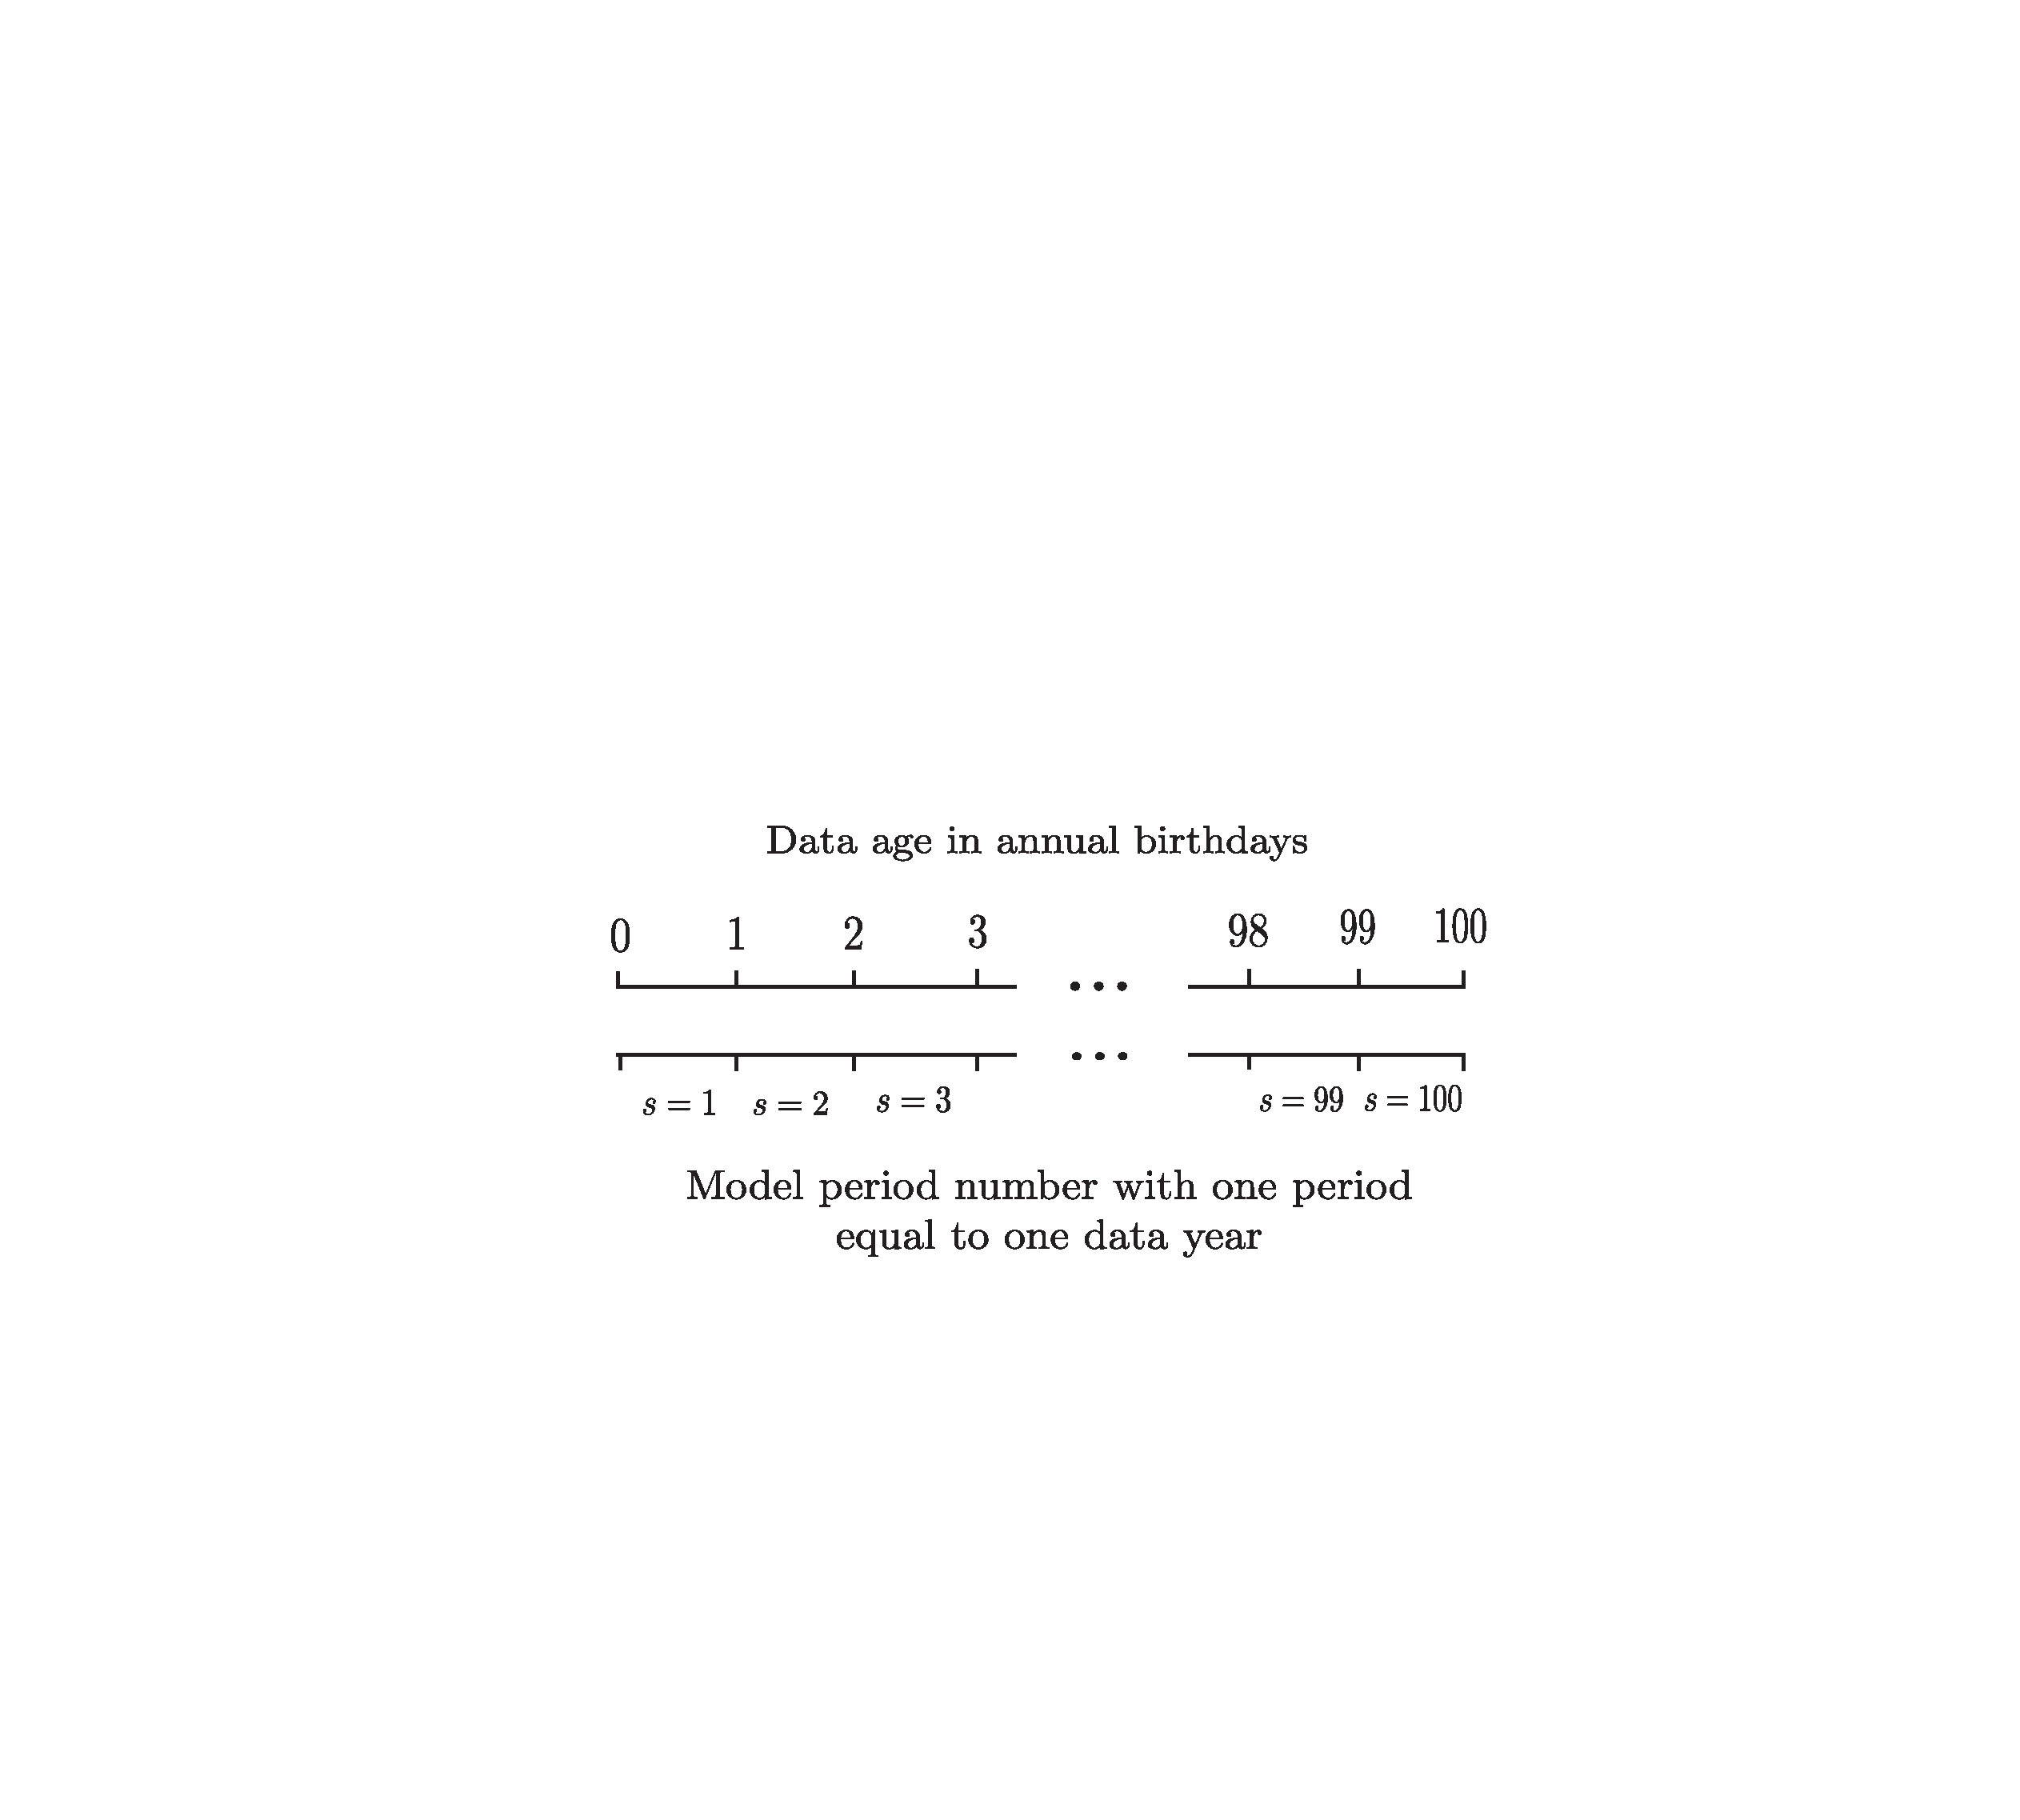
\includegraphics{images/FigPerTime.pdf}}}
  \end{figure}

  Our initial population distribution $\{\omega_{s,1}\}_{s=1}^{100}$ in Figure \ref{FigInitPopDist} comes from \citet{Census:2014} population estimates for both sexes for 2013. The fertility rates $\{f_s\}_{s=1}^{100}$ in Figure \ref{FigFertRates} come from \citet[Table 1]{NVSR:2010}. The mortality rates $\{\rho_s\}_{s=1}^{99}$ in Figure \ref{FigMortRates} come from the 2010 death probabilities in \citet{SocSec:2010}. We enforce a strict maximum age mortality rate of $\rho_{100}=1$ in our model.

  \begin{figure}[htbp]\centering \captionsetup{width=4.0in}
    \caption{\label{FigInitPopDist}\textbf{Initial population distribution $\omega_{s,1}$ by year, $1\leq s\leq 100$}}
    \fbox{\resizebox{4.0in}{2.8in}{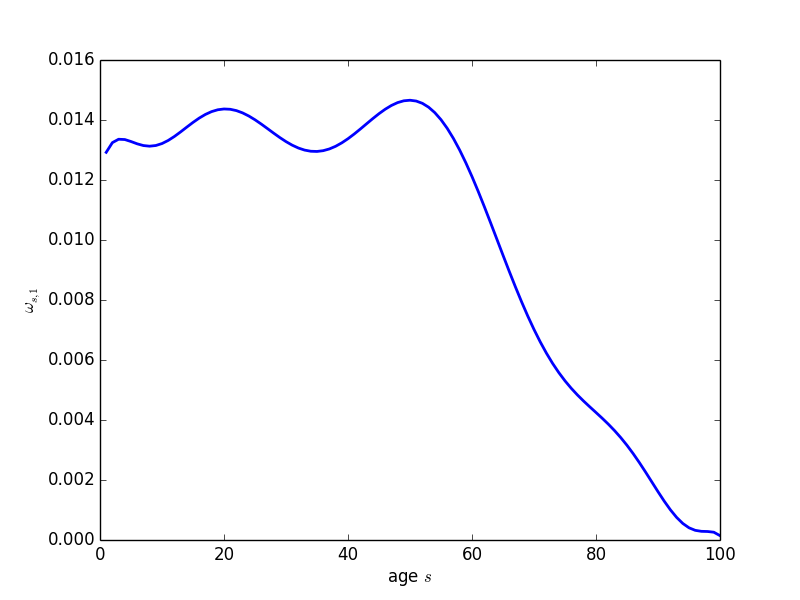
\includegraphics{images/omega_init.png}}}
  \end{figure}

  \begin{figure}[htbp]\centering \captionsetup{width=4.0in}
    \caption{\label{FigFertRates}\textbf{Fertility rates $f_s$ by year, $1\leq s\leq 100$}}
    \fbox{\resizebox{4.0in}{2.8in}{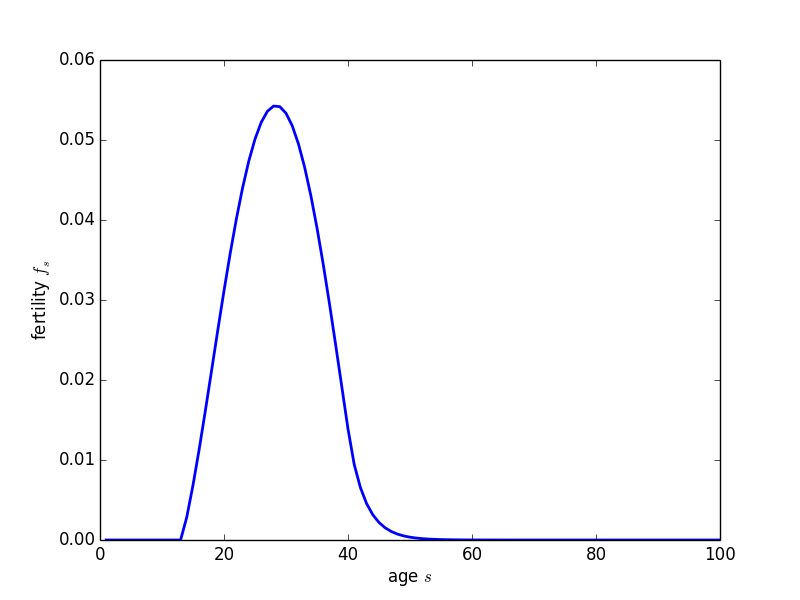
\includegraphics{images/fert_rates.png}}}
  \end{figure}

  \begin{figure}[htbp]\centering \captionsetup{width=4.0in}
    \caption{\label{FigMortRates}\textbf{Mortality rates $\rho_s$ by year, $1\leq s\leq 100$}}
    \fbox{\resizebox{4.0in}{2.8in}{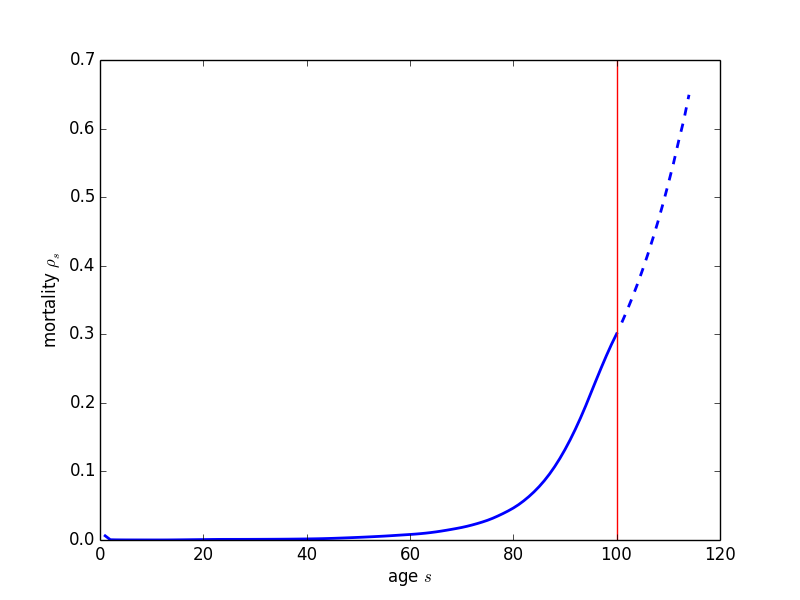
\includegraphics{images/mort_rates.png}}}
  \end{figure}

  The immigration rates $\{i_s\}_{s=1}^{99}$ in Figure \ref{FigImmigRates} are essentially residuals. We take total population for two consecutive years $N_t$ and $N_{t+1}$ and the population distribution by age in both of those years $\bm{\omega}_{t}$ and $\bm{\omega}_{t+1}$from the \citet{Census:2014} data. We then deduce the immigration rates $\{i_s\}_{s=1}^{99}$ using equation \eqref{EqPopLawofmotionStat}. We do this for three consecutive sets of years, so that our calibrated immigration rates by age are the average of our three years of deduced rates from the data for each age.

  \begin{figure}[htbp]\centering \captionsetup{width=4.0in}
    \caption{\label{FigImmigRates}\textbf{Immigration rates $i_s$ by year, $1\leq s\leq 100$}}
    \fbox{\resizebox{4.0in}{2.8in}{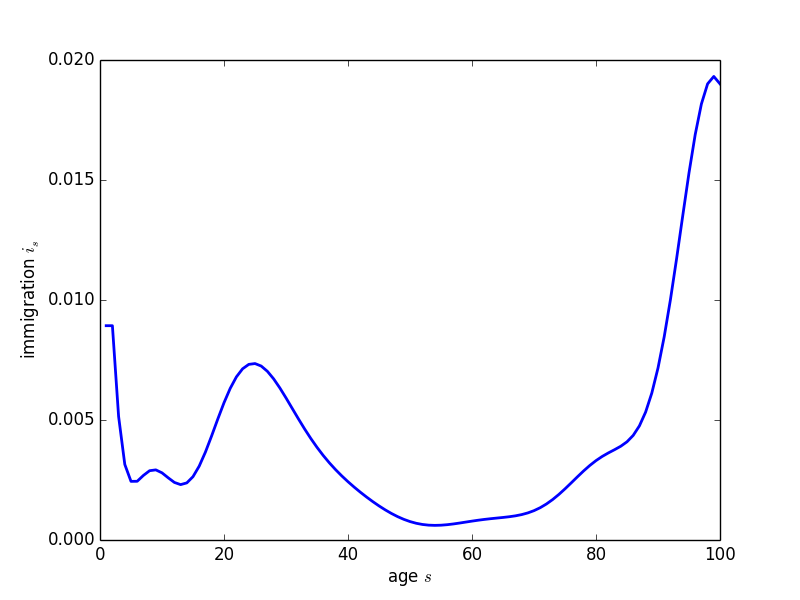
\includegraphics{images/imm_rates.png}}}
  \end{figure}

  Figure \ref{FigPopPath} shows the predicted time path of the total population $N_t$ given $\omega_{s,1}$ $f_s$, $i_s$, and $\rho_s$. Notice that the population approaches a constant growth rate. This is a result of the stationary population percent distribution $\bm{\bar{\omega}}$ eventually being reached. Figure \ref{FigSSpopdist} shows the steady-state population percent distribution by age $\bm{\bar{\omega}}$.

  \begin{figure}[htbp]\centering \captionsetup{width=4.0in}
    \caption{\label{FigPopPath}\textbf{Forecast time path of population growth rate $g_{n,t}$}}
    \fbox{\resizebox{4.0in}{2.8in}{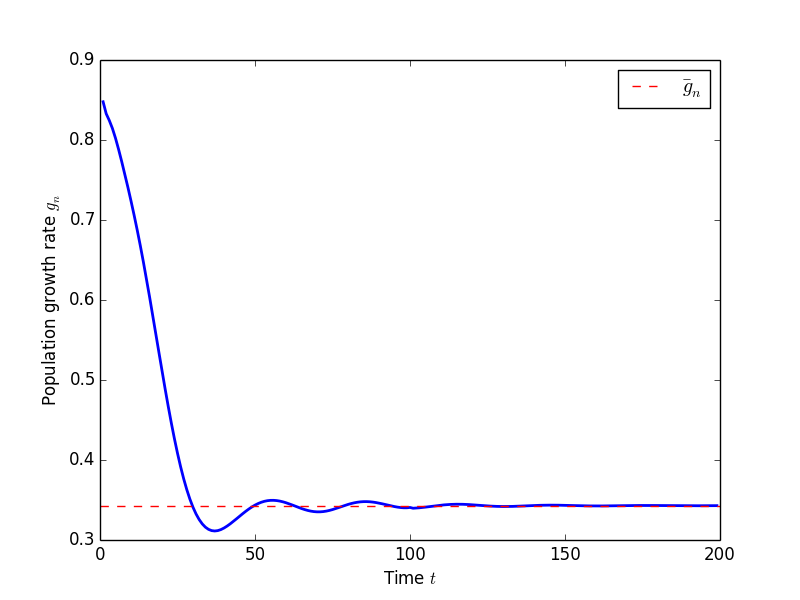
\includegraphics{images/Population_growthrate.png}}}
  \end{figure}

  \begin{figure}[htbp]\centering \captionsetup{width=4.0in}
    \caption{\label{FigSSpopdist}\textbf{Steady-state population percent distribution by age $\bm{\bar{\omega}}$}}
    \fbox{\resizebox{4.0in}{2.8in}{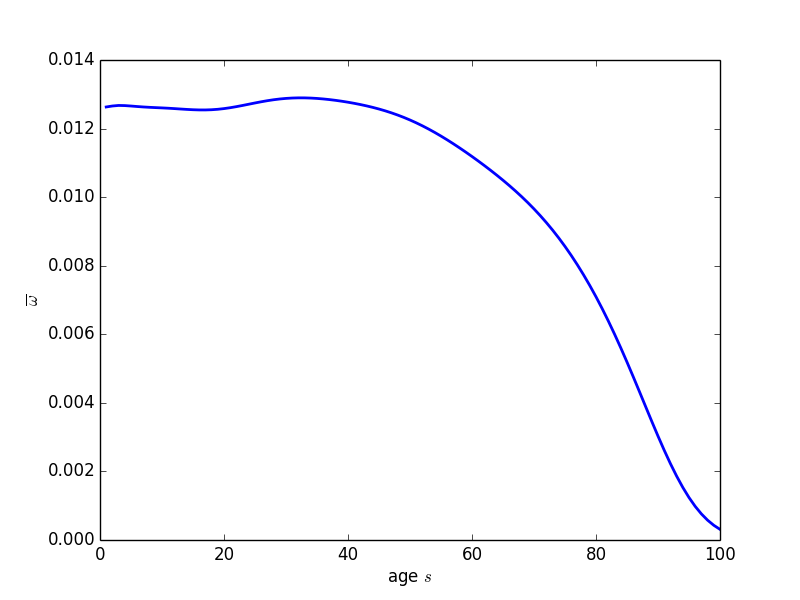
\includegraphics{images/omega_ss.png}}}
  \end{figure}
  \clearpage



\section{Incorporating Feedbacks with Micro Tax Simulations}\label{SecMicro}

  Follow this algorithm:
  \begin{itemize}
    \item Period 1
    \begin{itemize}
      \item Use current IRS public use sample.
      \item Run the following within-period routine
      \begin{itemize}
        \item Do the static tax analysis of this sample, save the results
        \item Summarize the public use sample by aggregating into bins over age and earnings ability
        \item Use this as a starting point for the dynamic macro model
        \item Get values for fundamental interest rates and effective wages for next period
      \end{itemize}
    \end{itemize}
  \item Period 2
    \begin{itemize}
      \item “Age” the public use data demographically by one year.
      \item Let wages and interest rates rise by the amounts predicted in the macro model.
      \item Rerun the within-period routine
    \end{itemize}
  \item Iterate over periods until end of forecast period is reached.
  \end{itemize}

\section{Calibration}
  \subsection{Tax Bend Points}
      We use IRS data which summarizes individual tax returns for 2011 by 19 income categories and 4 filing statuses.  For each filing status we fit the mapping from reported income into adjusted gross income (AGI) using a sufficiently high-order polynomial.  We then use this function to solve for the income level which corresponds to each of the five bend points in the tax code for each filing type.
      \begin{table}[ht]
        \caption{AGI and Income Bend Points}
        \label{Calib_Bend_Tab1}
        \centering
        AGI Bend Points
        \begin{tabular}{|r|r|r|r|r|} \hline
          Tax rate & Married Joint & Married Separate & Head of Household & Single \\ \hline
          10\% & 17,400 & 8700 & 12,400 & 8700 \\ \hline
          15\% & 70,700 & 35,350 & 47,350 & 35,350 \\ \hline
          25\% & 142,700 & 71,350 & 122,300 & 85,650 \\ \hline
          28\% & 217,450 & 108,725 & 198,050 & 178,650 \\ \hline
          33\% & 388,350 & 194,175 & 388,350 & 388,350 \\ \hline
        \end{tabular}
        \\
        Corresponding Reported Income Bendpoints
        \begin{tabular}{|r|r|r|r|r|} \hline
          Tax rate & Married Joint & Married Separate & Head of Household & Single \\ \hline
          0\%  & 5850  & 91 & 756 & 1435 \\ \hline
          10\% & 22,932 & 8591 & 12,911 & 9956 \\ \hline
          15\% & 75,181 & 34,592 & 47,023 & 36,021 \\ \hline
          25\% & 145,866 & 69,768 & 120,200 & 85,244 \\ \hline
          28\% & 219,162 & 106,245 & 194,176 & 176,270 \\ \hline
          33\% & 386,798 & 189,674 & 380,043 & 381,524 \\ \hline
        \end{tabular}
      \end{table}

      We then fit a bivariate probability density function over income and filing type from the data.  For each bendpoint we calculate the probability density at that bendpoint and use these as weights in a weighted average over filing types to generate an aggregate bendpoint.
      \begin{table}[ht]
        \caption{Aggregated Bend Points}
        \label{Calib_Bend_Tab2}
        \centering
        \begin{tabular}{|r|r|} \hline
          Tax rate & Bend Point \\ \hline
          0\% & 2889 \\ \hline
          10\% & 15,116 \\ \hline
          15\% & 52,580 \\ \hline
          25\% & 114,552 \\ \hline
          28\% & 196,201 \\ \hline
          33\% & 380,657 \\ \hline
        \end{tabular}
      \end{table}

% Bibliography:
\clearpage
\bibliography{OG_USA_Guide}
\index{Bibliography@\emph{Bibliography}}%

\printindex

\end{document}
